\documentclass[twoside]{article}

\usepackage{aistats2021}
% If your paper is accepted, change the options for the package
% aistats2021 as follows:
%
%\usepackage[accepted]{aistats2021}
%
% This option will print headings for the title of your paper and
% headings for the authors names, plus a copyright note at the end of
% the first column of the first page.

% If you set papersize explicitly, activate the following three lines:
%\special{papersize = 8.5in, 11in}
%\setlength{\pdfpageheight}{11in}
%\setlength{\pdfpagewidth}{8.5in}

% If you use natbib package, activate the following three lines:
%\usepackage[round]{natbib}
%\renewcommand{\bibname}{References}
%\renewcommand{\bibsection}{\subsubsection*{\bibname}}

% If you use BibTeX in apalike style, activate the following line:
\bibliographystyle{apalike}

%%%%%% NEW MATH DEFINITIONS %%%%%

\usepackage{amsmath,amsfonts,bm}

% Mark sections of captions for referring to divisions of figures
\newcommand{\figleft}{{\em (Left)}}
\newcommand{\figcenter}{{\em (Center)}}
\newcommand{\figright}{{\em (Right)}}
\newcommand{\figtop}{{\em (Top)}}
\newcommand{\figbottom}{{\em (Bottom)}}
\newcommand{\captiona}{{\em (a)}}
\newcommand{\captionb}{{\em (b)}}
\newcommand{\captionc}{{\em (c)}}
\newcommand{\captiond}{{\em (d)}}

% Highlight a newly defined term
\newcommand{\newterm}[1]{{\bf #1}}


% Figure reference, lower-case.
\def\figref#1{figure~\ref{#1}}
% Figure reference, capital. For start of sentence
\def\Figref#1{Figure~\ref{#1}}
\def\twofigref#1#2{figures \ref{#1} and \ref{#2}}
\def\quadfigref#1#2#3#4{figures \ref{#1}, \ref{#2}, \ref{#3} and \ref{#4}}
% Section reference, lower-case.
\def\secref#1{section~\ref{#1}}
% Section reference, capital.
\def\Secref#1{Section~\ref{#1}}
% Reference to two sections.
\def\twosecrefs#1#2{sections \ref{#1} and \ref{#2}}
% Reference to three sections.
\def\secrefs#1#2#3{sections \ref{#1}, \ref{#2} and \ref{#3}}
% Reference to an equation, lower-case.
\def\eqref#1{equation~\ref{#1}}
% Reference to an equation, upper case
\def\Eqref#1{Equation~\ref{#1}}
% A raw reference to an equation---avoid using if possible
\def\plaineqref#1{\ref{#1}}
% Reference to a chapter, lower-case.
\def\chapref#1{chapter~\ref{#1}}
% Reference to an equation, upper case.
\def\Chapref#1{Chapter~\ref{#1}}
% Reference to a range of chapters
\def\rangechapref#1#2{chapters\ref{#1}--\ref{#2}}
% Reference to an algorithm, lower-case.
\def\algref#1{algorithm~\ref{#1}}
% Reference to an algorithm, upper case.
\def\Algref#1{Algorithm~\ref{#1}}
\def\twoalgref#1#2{algorithms \ref{#1} and \ref{#2}}
\def\Twoalgref#1#2{Algorithms \ref{#1} and \ref{#2}}
% Reference to a part, lower case
\def\partref#1{part~\ref{#1}}
% Reference to a part, upper case
\def\Partref#1{Part~\ref{#1}}
\def\twopartref#1#2{parts \ref{#1} and \ref{#2}}

\def\ceil#1{\lceil #1 \rceil}
\def\floor#1{\lfloor #1 \rfloor}
\def\1{\bm{1}}
\newcommand{\train}{\mathcal{D}}
\newcommand{\valid}{\mathcal{D_{\mathrm{valid}}}}
\newcommand{\test}{\mathcal{D_{\mathrm{test}}}}

\def\eps{{\epsilon}}


% Random variables
\def\reta{{\textnormal{$\eta$}}}
\def\ra{{\textnormal{a}}}
\def\rb{{\textnormal{b}}}
\def\rc{{\textnormal{c}}}
\def\rd{{\textnormal{d}}}
\def\re{{\textnormal{e}}}
\def\rf{{\textnormal{f}}}
\def\rg{{\textnormal{g}}}
\def\rh{{\textnormal{h}}}
\def\ri{{\textnormal{i}}}
\def\rj{{\textnormal{j}}}
\def\rk{{\textnormal{k}}}
\def\rl{{\textnormal{l}}}
% rm is already a command, just don't name any random variables m
\def\rn{{\textnormal{n}}}
\def\ro{{\textnormal{o}}}
\def\rp{{\textnormal{p}}}
\def\rq{{\textnormal{q}}}
\def\rr{{\textnormal{r}}}
\def\rs{{\textnormal{s}}}
\def\rt{{\textnormal{t}}}
\def\ru{{\textnormal{u}}}
\def\rv{{\textnormal{v}}}
\def\rw{{\textnormal{w}}}
\def\rx{{\textnormal{x}}}
\def\ry{{\textnormal{y}}}
\def\rz{{\textnormal{z}}}

% Random vectors
\def\rvepsilon{{\mathbf{\epsilon}}}
\def\rvtheta{{\mathbf{\theta}}}
\def\rva{{\mathbf{a}}}
\def\rvb{{\mathbf{b}}}
\def\rvc{{\mathbf{c}}}
\def\rvd{{\mathbf{d}}}
\def\rve{{\mathbf{e}}}
\def\rvf{{\mathbf{f}}}
\def\rvg{{\mathbf{g}}}
\def\rvh{{\mathbf{h}}}
\def\rvu{{\mathbf{i}}}
\def\rvj{{\mathbf{j}}}
\def\rvk{{\mathbf{k}}}
\def\rvl{{\mathbf{l}}}
\def\rvm{{\mathbf{m}}}
\def\rvn{{\mathbf{n}}}
\def\rvo{{\mathbf{o}}}
\def\rvp{{\mathbf{p}}}
\def\rvq{{\mathbf{q}}}
\def\rvr{{\mathbf{r}}}
\def\rvs{{\mathbf{s}}}
\def\rvt{{\mathbf{t}}}
\def\rvu{{\mathbf{u}}}
\def\rvv{{\mathbf{v}}}
\def\rvw{{\mathbf{w}}}
\def\rvx{{\mathbf{x}}}
\def\rvy{{\mathbf{y}}}
\def\rvz{{\mathbf{z}}}

% Elements of random vectors
\def\erva{{\textnormal{a}}}
\def\ervb{{\textnormal{b}}}
\def\ervc{{\textnormal{c}}}
\def\ervd{{\textnormal{d}}}
\def\erve{{\textnormal{e}}}
\def\ervf{{\textnormal{f}}}
\def\ervg{{\textnormal{g}}}
\def\ervh{{\textnormal{h}}}
\def\ervi{{\textnormal{i}}}
\def\ervj{{\textnormal{j}}}
\def\ervk{{\textnormal{k}}}
\def\ervl{{\textnormal{l}}}
\def\ervm{{\textnormal{m}}}
\def\ervn{{\textnormal{n}}}
\def\ervo{{\textnormal{o}}}
\def\ervp{{\textnormal{p}}}
\def\ervq{{\textnormal{q}}}
\def\ervr{{\textnormal{r}}}
\def\ervs{{\textnormal{s}}}
\def\ervt{{\textnormal{t}}}
\def\ervu{{\textnormal{u}}}
\def\ervv{{\textnormal{v}}}
\def\ervw{{\textnormal{w}}}
\def\ervx{{\textnormal{x}}}
\def\ervy{{\textnormal{y}}}
\def\ervz{{\textnormal{z}}}

% Random matrices
\def\rmA{{\mathbf{A}}}
\def\rmB{{\mathbf{B}}}
\def\rmC{{\mathbf{C}}}
\def\rmD{{\mathbf{D}}}
\def\rmE{{\mathbf{E}}}
\def\rmF{{\mathbf{F}}}
\def\rmG{{\mathbf{G}}}
\def\rmH{{\mathbf{H}}}
\def\rmI{{\mathbf{I}}}
\def\rmJ{{\mathbf{J}}}
\def\rmK{{\mathbf{K}}}
\def\rmL{{\mathbf{L}}}
\def\rmM{{\mathbf{M}}}
\def\rmN{{\mathbf{N}}}
\def\rmO{{\mathbf{O}}}
\def\rmP{{\mathbf{P}}}
\def\rmQ{{\mathbf{Q}}}
\def\rmR{{\mathbf{R}}}
\def\rmS{{\mathbf{S}}}
\def\rmT{{\mathbf{T}}}
\def\rmU{{\mathbf{U}}}
\def\rmV{{\mathbf{V}}}
\def\rmW{{\mathbf{W}}}
\def\rmX{{\mathbf{X}}}
\def\rmY{{\mathbf{Y}}}
\def\rmZ{{\mathbf{Z}}}

% Elements of random matrices
\def\ermA{{\textnormal{A}}}
\def\ermB{{\textnormal{B}}}
\def\ermC{{\textnormal{C}}}
\def\ermD{{\textnormal{D}}}
\def\ermE{{\textnormal{E}}}
\def\ermF{{\textnormal{F}}}
\def\ermG{{\textnormal{G}}}
\def\ermH{{\textnormal{H}}}
\def\ermI{{\textnormal{I}}}
\def\ermJ{{\textnormal{J}}}
\def\ermK{{\textnormal{K}}}
\def\ermL{{\textnormal{L}}}
\def\ermM{{\textnormal{M}}}
\def\ermN{{\textnormal{N}}}
\def\ermO{{\textnormal{O}}}
\def\ermP{{\textnormal{P}}}
\def\ermQ{{\textnormal{Q}}}
\def\ermR{{\textnormal{R}}}
\def\ermS{{\textnormal{S}}}
\def\ermT{{\textnormal{T}}}
\def\ermU{{\textnormal{U}}}
\def\ermV{{\textnormal{V}}}
\def\ermW{{\textnormal{W}}}
\def\ermX{{\textnormal{X}}}
\def\ermY{{\textnormal{Y}}}
\def\ermZ{{\textnormal{Z}}}

% Vectors
\def\vzero{{\bm{0}}}
\def\vone{{\bm{1}}}
\def\vmu{{\bm{\mu}}}
\def\vtheta{{\bm{\theta}}}
\def\va{{\bm{a}}}
\def\vb{{\bm{b}}}
\def\vc{{\bm{c}}}
\def\vd{{\bm{d}}}
\def\ve{{\bm{e}}}
\def\vf{{\bm{f}}}
\def\vg{{\bm{g}}}
\def\vh{{\bm{h}}}
\def\vi{{\bm{i}}}
\def\vj{{\bm{j}}}
\def\vk{{\bm{k}}}
\def\vl{{\bm{l}}}
\def\vm{{\bm{m}}}
\def\vn{{\bm{n}}}
\def\vo{{\bm{o}}}
\def\vp{{\bm{p}}}
\def\vq{{\bm{q}}}
\def\vr{{\bm{r}}}
\def\vs{{\bm{s}}}
\def\vt{{\bm{t}}}
\def\vu{{\bm{u}}}
\def\vv{{\bm{v}}}
\def\vw{{\bm{w}}}
\def\vx{{\bm{x}}}
\def\vy{{\bm{y}}}
\def\vz{{\bm{z}}}

% Elements of vectors
\def\evalpha{{\alpha}}
\def\evbeta{{\beta}}
\def\evepsilon{{\epsilon}}
\def\evlambda{{\lambda}}
\def\evomega{{\omega}}
\def\evmu{{\mu}}
\def\evpsi{{\psi}}
\def\evsigma{{\sigma}}
\def\evtheta{{\theta}}
\def\eva{{a}}
\def\evb{{b}}
\def\evc{{c}}
\def\evd{{d}}
\def\eve{{e}}
\def\evf{{f}}
\def\evg{{g}}
\def\evh{{h}}
\def\evi{{i}}
\def\evj{{j}}
\def\evk{{k}}
\def\evl{{l}}
\def\evm{{m}}
\def\evn{{n}}
\def\evo{{o}}
\def\evp{{p}}
\def\evq{{q}}
\def\evr{{r}}
\def\evs{{s}}
\def\evt{{t}}
\def\evu{{u}}
\def\evv{{v}}
\def\evw{{w}}
\def\evx{{x}}
\def\evy{{y}}
\def\evz{{z}}

% Matrix
\def\mA{{\bm{A}}}
\def\mB{{\bm{B}}}
\def\mC{{\bm{C}}}
\def\mD{{\bm{D}}}
\def\mE{{\bm{E}}}
\def\mF{{\bm{F}}}
\def\mG{{\bm{G}}}
\def\mH{{\bm{H}}}
\def\mI{{\bm{I}}}
\def\mJ{{\bm{J}}}
\def\mK{{\bm{K}}}
\def\mL{{\bm{L}}}
\def\mM{{\bm{M}}}
\def\mN{{\bm{N}}}
\def\mO{{\bm{O}}}
\def\mP{{\bm{P}}}
\def\mQ{{\bm{Q}}}
\def\mR{{\bm{R}}}
\def\mS{{\bm{S}}}
\def\mT{{\bm{T}}}
\def\mU{{\bm{U}}}
\def\mV{{\bm{V}}}
\def\mW{{\bm{W}}}
\def\mX{{\bm{X}}}
\def\mY{{\bm{Y}}}
\def\mZ{{\bm{Z}}}
\def\mBeta{{\bm{\beta}}}
\def\mPhi{{\bm{\Phi}}}
\def\mLambda{{\bm{\Lambda}}}
\def\mSigma{{\bm{\Sigma}}}

% Tensor
\DeclareMathAlphabet{\mathsfit}{\encodingdefault}{\sfdefault}{m}{sl}
\SetMathAlphabet{\mathsfit}{bold}{\encodingdefault}{\sfdefault}{bx}{n}
\newcommand{\tens}[1]{\bm{\mathsfit{#1}}}
\def\tA{{\tens{A}}}
\def\tB{{\tens{B}}}
\def\tC{{\tens{C}}}
\def\tD{{\tens{D}}}
\def\tE{{\tens{E}}}
\def\tF{{\tens{F}}}
\def\tG{{\tens{G}}}
\def\tH{{\tens{H}}}
\def\tI{{\tens{I}}}
\def\tJ{{\tens{J}}}
\def\tK{{\tens{K}}}
\def\tL{{\tens{L}}}
\def\tM{{\tens{M}}}
\def\tN{{\tens{N}}}
\def\tO{{\tens{O}}}
\def\tP{{\tens{P}}}
\def\tQ{{\tens{Q}}}
\def\tR{{\tens{R}}}
\def\tS{{\tens{S}}}
\def\tT{{\tens{T}}}
\def\tU{{\tens{U}}}
\def\tV{{\tens{V}}}
\def\tW{{\tens{W}}}
\def\tX{{\tens{X}}}
\def\tY{{\tens{Y}}}
\def\tZ{{\tens{Z}}}


% Graph
\def\gA{{\mathcal{A}}}
\def\gB{{\mathcal{B}}}
\def\gC{{\mathcal{C}}}
\def\gD{{\mathcal{D}}}
\def\gE{{\mathcal{E}}}
\def\gF{{\mathcal{F}}}
\def\gG{{\mathcal{G}}}
\def\gH{{\mathcal{H}}}
\def\gI{{\mathcal{I}}}
\def\gJ{{\mathcal{J}}}
\def\gK{{\mathcal{K}}}
\def\gL{{\mathcal{L}}}
\def\gM{{\mathcal{M}}}
\def\gN{{\mathcal{N}}}
\def\gO{{\mathcal{O}}}
\def\gP{{\mathcal{P}}}
\def\gQ{{\mathcal{Q}}}
\def\gR{{\mathcal{R}}}
\def\gS{{\mathcal{S}}}
\def\gT{{\mathcal{T}}}
\def\gU{{\mathcal{U}}}
\def\gV{{\mathcal{V}}}
\def\gW{{\mathcal{W}}}
\def\gX{{\mathcal{X}}}
\def\gY{{\mathcal{Y}}}
\def\gZ{{\mathcal{Z}}}

% Sets
\def\sA{{\mathbb{A}}}
\def\sB{{\mathbb{B}}}
\def\sC{{\mathbb{C}}}
\def\sD{{\mathbb{D}}}
% Don't use a set called E, because this would be the same as our symbol
% for expectation.
\def\sF{{\mathbb{F}}}
\def\sG{{\mathbb{G}}}
\def\sH{{\mathbb{H}}}
\def\sI{{\mathbb{I}}}
\def\sJ{{\mathbb{J}}}
\def\sK{{\mathbb{K}}}
\def\sL{{\mathbb{L}}}
\def\sM{{\mathbb{M}}}
\def\sN{{\mathbb{N}}}
\def\sO{{\mathbb{O}}}
\def\sP{{\mathbb{P}}}
\def\sQ{{\mathbb{Q}}}
\def\sR{{\mathbb{R}}}
\def\sS{{\mathbb{S}}}
\def\sT{{\mathbb{T}}}
\def\sU{{\mathbb{U}}}
\def\sV{{\mathbb{V}}}
\def\sW{{\mathbb{W}}}
\def\sX{{\mathbb{X}}}
\def\sY{{\mathbb{Y}}}
\def\sZ{{\mathbb{Z}}}

% Entries of a matrix
\def\emLambda{{\Lambda}}
\def\emA{{A}}
\def\emB{{B}}
\def\emC{{C}}
\def\emD{{D}}
\def\emE{{E}}
\def\emF{{F}}
\def\emG{{G}}
\def\emH{{H}}
\def\emI{{I}}
\def\emJ{{J}}
\def\emK{{K}}
\def\emL{{L}}
\def\emM{{M}}
\def\emN{{N}}
\def\emO{{O}}
\def\emP{{P}}
\def\emQ{{Q}}
\def\emR{{R}}
\def\emS{{S}}
\def\emT{{T}}
\def\emU{{U}}
\def\emV{{V}}
\def\emW{{W}}
\def\emX{{X}}
\def\emY{{Y}}
\def\emZ{{Z}}
\def\emSigma{{\Sigma}}

% Same font as tensor, without \bm wrapper
\newcommand{\etens}[1]{\mathsfit{#1}}
\def\etLambda{{\etens{\Lambda}}}
\def\etA{{\etens{A}}}
\def\etB{{\etens{B}}}
\def\etC{{\etens{C}}}
\def\etD{{\etens{D}}}
\def\etE{{\etens{E}}}
\def\etF{{\etens{F}}}
\def\etG{{\etens{G}}}
\def\etH{{\etens{H}}}
\def\etI{{\etens{I}}}
\def\etJ{{\etens{J}}}
\def\etK{{\etens{K}}}
\def\etL{{\etens{L}}}
\def\etM{{\etens{M}}}
\def\etN{{\etens{N}}}
\def\etO{{\etens{O}}}
\def\etP{{\etens{P}}}
\def\etQ{{\etens{Q}}}
\def\etR{{\etens{R}}}
\def\etS{{\etens{S}}}
\def\etT{{\etens{T}}}
\def\etU{{\etens{U}}}
\def\etV{{\etens{V}}}
\def\etW{{\etens{W}}}
\def\etX{{\etens{X}}}
\def\etY{{\etens{Y}}}
\def\etZ{{\etens{Z}}}

% The true underlying data generating distribution
\newcommand{\pdata}{p_{\rm{data}}}
% The empirical distribution defined by the training set
\newcommand{\ptrain}{\hat{p}_{\rm{data}}}
\newcommand{\Ptrain}{\hat{P}_{\rm{data}}}
% The model distribution
\newcommand{\pmodel}{p_{\rm{model}}}
\newcommand{\Pmodel}{P_{\rm{model}}}
\newcommand{\ptildemodel}{\tilde{p}_{\rm{model}}}
% Stochastic autoencoder distributions
\newcommand{\pencode}{p_{\rm{encoder}}}
\newcommand{\pdecode}{p_{\rm{decoder}}}
\newcommand{\precons}{p_{\rm{reconstruct}}}

\newcommand{\laplace}{\mathrm{Laplace}} % Laplace distribution

%\newcommand{\E}{\mathbb{E}}
\newcommand{\Ls}{\mathcal{L}}
\newcommand{\R}{\mathbb{R}}
\newcommand{\emp}{\tilde{p}}
\newcommand{\lr}{\alpha}
\newcommand{\reg}{\lambda}
\newcommand{\rect}{\mathrm{rectifier}}
\newcommand{\softmax}{\mathrm{softmax}}
\newcommand{\sigmoid}{\sigma}
\newcommand{\softplus}{\zeta}
\newcommand{\KL}{D_{\mathrm{KL}}}
%%%\newcommand{\Var}{\mathrm{Var}}
\newcommand{\standarderror}{\mathrm{SE}}
\newcommand{\Cov}{\mathrm{Cov}}

% Wolfram Mathworld says $L^2$ is for function spaces and $\ell^2$ is for vectors
% But then they seem to use $L^2$ for vectors throughout the site, and so does
% wikipedia.
\newcommand{\normlzero}{L^0}
\newcommand{\normlone}{L^1}
\newcommand{\normltwo}{L^2}
\newcommand{\normlp}{L^p}
\newcommand{\normmax}{L^\infty}

\newcommand{\parents}{Pa} % See usage in notation.tex. Chosen to match Daphne's book.

\DeclareMathOperator*{\argmax}{arg\,max}
\DeclareMathOperator*{\argmin}{arg\,min}

\DeclareMathOperator{\sign}{sign}
\DeclareMathOperator{\Tr}{Tr}
\let\ab\allowbreak


\usepackage{hyperref}
\usepackage{url}
\usepackage{amsmath}
\usepackage{amssymb}
\usepackage{amsthm}
\usepackage{algorithm}
\usepackage{algorithmic}
\usepackage{graphicx}
\usepackage{xcolor}
%\usepackage[colorinlistoftodos]{todonotes}
%\usepackage[colorlinks=true, allcolors=blue]{hyperref}
%\usepackage{accents}
\usepackage{wrapfig}
\usepackage[thinlines]{easytable}
\usepackage{titlesec}
\usepackage{subcaption}
\usepackage{mathtools}
\usepackage{bold-extra}
\usepackage{bm}
\usepackage{booktabs}

\newcommand{\ubar}[1]{\underaccent{\bar}{#1}}
  
\newcommand{\steve}[1]{{\color{magenta} { [Steve: #1]}}}
\newcommand{\bcw}[1]{{\color{orange} { [Ben: #1]}}}
\newcommand{\mayee}[1]{{\color{green} { [Mayee: #1]}}}
\newcommand{\chris}[1]{\textcolor{red}{[Chris: #1]}}
\newcommand{\todo}[1]{{\color{red} {[TODO: #1]}}}

\newcommand{\fix}{\marginpar{FIX}}
\newcommand{\new}{\marginpar{NEW}}

\newtheorem{theorem}{Theorem}
\newtheorem{lemma}{Lemma}
\newtheorem{corollary}{Corollary}
\newtheorem{observation}{Observation}
\newtheorem{definition}{Definition}
\newtheorem{example}{Example}
\newtheorem{proposition}{Proposition}
\newtheorem{remark}{Remark}
\newtheorem{assumption}{Assumption}

%% OPERATORS:
\newcommand{\norm}[1]{\left|\left|#1\right|\right|}
\newcommand{\argmin}[2]{\textrm{argmin}_{#1}~#2}
\newcommand{\argmax}[2]{\textrm{argmax}_{#1}~#2}
% Inner product
\newcommand{\ip}[2]{\left\langle#1, #2\right\rangle}
% Trace
\newcommand{\tr}{\textrm{tr}}
% Expected value
\newcommand{\E}[2]{\mathbb{E}_{#1}\left[#2\right]}
% Sample mean
\newcommand{\Ehat}[1]{\hat{\mathbb{E}}\left[#1\right]}
% Variance
\newcommand{\Var}[2]{\mathrm{Var}_{#1}\left(#2\right)}
% Covariance
%\newcommand{\Cov}[2]{\textrm{\textbf{Cov}}_{#1}\left[#2\right]}
% Indicator
\newcommand{\ind}[1]{\mathbbm{1}\left\{#1\right\}}
\newcommand{\indpm}[1]{\mathbbm{1}^{\pm}\left\{#1\right\}}
% sech
\newcommand{\sech}[0]{\textrm{sech}}
% diag
\newcommand{\diagm}[1]{\textrm{diagm}\left(#1\right)}
% supp
\newcommand{\supp}{\text{supp}}
% independent
\newcommand\independent{\protect\mathpalette{\protect\independenT}{\perp}}
\def\independenT#1#2{\mathrel{\rlap{$#1#2$}\mkern2mu{#1#2}}}


\newcommand{\Eprime}[2]{\mathbb{E}'_{#1}\left[#2\right]}
\newcommand{\Etilde}[2]{\widetilde{\mathbb{E}}_{#1}\left[#2\right]}

\newcommand{\Ptilde}[0]{\widetilde{\Pr}}
\newcommand{\Pbar}[0]{\overline{\Pr}}
\newcommand{\Phat}[0]{\hat{\Pr}}


\newcommand{\T}[0]{\mathcal{T}}





%% VARIABLES:
% See Glossary of Symbols (Appendix A.1)
\newcommand{\x}[0]{X}
\newcommand{\p}[0]{\mathcal{P}}
\newcommand{\y}[0]{Y}
\newcommand{\lf}[0]{\lambda}
\newcommand{\lfc}[0]{\Lambda}
\newcommand{\acc}[0]{\alpha}
\newcommand{\X}[0]{\mathcal{X}}
\newcommand{\D}[0]{\mathcal{D}}
\newcommand{\N}[0]{\mathcal{N}}

\usepackage{natbib}
%\setcitestyle{square}
\usepackage{enumitem}
\setlist{nosep}

\begin{document}

% If your paper is accepted and the title of your paper is very long,
% the style will print as headings an error message. Use the following
% command to supply a shorter title of your paper so that it can be
% used as headings.
%
%\runningtitle{I use this title instead because the last one was very long}

% If your paper is accepted and the number of authors is large, the
% style will print as headings an error message. Use the following
% command to supply a shorter version of the authors names so that
% they can be used as headings (for example, use only the surnames)
%
%\runningauthor{Surname 1, Surname 2, Surname 3, ...., Surname n}

\singlecolumnfalse

\twocolumn[

%\aistatstitle{On the Value of Supervision in Data Programming}
\aistatstitle{Comparing the Value of Labeled and Unlabeled Data \\in Method-of-Moments Latent Variable Estimation}

\aistatsauthor{ Author 1 \And Author 2 \And  Author 3 }

\aistatsaddress{ Institution 1 \And  Institution 2 \And Institution 3 } ]

\begin{abstract}
  Labeling data for modern machine learning is expensive and time-consuming. Latent variable models are used to infer labels from weaker, easier-to-acquire sources operating on unlabeled data.
Such models can also be trained using labeled data, presenting a key question: should a user invest in few labeled or many unlabeled points? We answer this via a framework centered on model misspecification in method-of-moments latent variable estimation.
%
Our core result is an exact bias-variance decomposition of the generalization error, which shows that the unlabeled-only approach incurs additional bias under misspecification. We introduce a correction that provably removes this bias in certain cases.
%
We apply our decomposition to three scenarios---well-specified, misspecified, and corrected models---to 1) choose between  labeled and unlabeled data and 2) learn from a combination. We observe theoretically and with synthetic experiments that for well-specified models, labeled points are worth a constant factor more than unlabeled points. With misspecification, their relative value is higher due to the additional bias but is reduced with correction. We also apply our approach to study real-world weak supervision techniques for dataset construction.


%OLD
%Labeling data for modern machine learning is expensive and time-consuming while unlabeled data is is generally less informative but easier to acquire, presenting a tradeoff. %\steve{I think this first sentence could be improved to make the tradeoff make more sense: ``Labeling data for modern machine learning is expensive and time-consuming while unlabeled data is generally less informative but easier to acquire, presenting a tradeoff''} %This presents a key tradeoff: should a user invest in few labeled or many unlabeled points? 
%We consider probabilistic models for generating labels, for which both labeled and unlabeled data can be used as input. In the former case, these models have directly computable parameters, while in the latter, they reduce to \textit{latent variable models} where approaches such as method-of-moments are needed to infer labels. 
%Motivated by weak supervision as an application, we study the impact of model misspecification on method-of-moments estimators and their ability to generate accurate labels. Our core result is an exact bias-variance decomposition of the generalization error for such models, which shows that the unlabeled-only approach incurs additional bias under misspecification. We introduce a corrected estimator that provably removes this bias under certain conditions.
%We apply our decomposition framework to three scenarios---well-specified models, misspecified models, and misspecified models with our corrected estimator---to 1) assess labeled vs unlabeled data and 2) learn from a combination of both. We observe theoretically and with synthetic experiments that for well-specified models, labeled points are worth a constant factor more than unlabeled points in terms of generalization error. For misspecified models, their relative value based on our framework is higher due to the additional bias in the unlabeled approach but can be reduced when our correction mechanism is applied.


% OLD OLD
%Labeling data for modern machine learning is expensive and time-consuming. Weak supervision (WS) combines unlabeled data and weak sources to learn a model that generates a large labeled dataset. Such models can also benefit from labeled data, presenting a key tradeoff: should a user invest in few labeled or many unlabeled points? 
%We present a framework centered on model misspecification in WS algorithms. Our core result is an exact bias-variance decomposition of the generalization error, which shows that the unlabeled-only approach incurs additional bias under misspecification. We introduce a correction mechanism that is broadly applicable to method-of-moments approaches and provably removes this bias under certain conditions.
%We apply our decomposition framework to three scenarios---well-specified models, misspecified models, and misspecified models with our correction mechanism---to 1) choose between using labeled vs unlabeled data and 2) learn from a combination of both. We observe theoretically and with synthetic experiments that for well-specified models, labeled points are worth a constant factor more than unlabeled points in terms of generalization error. For misspecified models, their relative value based on our framework is higher due to the additional bias in the unlabeled approach but can be reduced when our correction mechanism is applied.

%the relative amount of unlabeled data to match an improvement in generalization error with additional labeled data is a small constant, while for misspecified models, the asymptotic bias of the unlabeled-only approach grows with more dependencies.



%% Previous version
%Labeling data for modern machine learning is expensive and time-consuming. Weak supervision (WS) combines unlabeled data and weak sources to learn a model that generates a large labeled dataset. Such models can also benefit from labeled data, presenting a key tradeoff: should a user invest in few labeled or many unlabeled points? 
%We answer this via a framework centered on model misspecification in WS that is broadly applicable to method-of-moments estimators. Our core result is an exact bias-variance decomposition of the generalization error, which shows that the unlabeled-only approach incurs additional bias under misspecification. We then give a correction mechanism.
%We apply our framework to three scenarios---well-specified, misspecified, and corrected models---to 1) assess the value of labeled vs unlabeled data and 2) learn from a combination of both. In line with our error decomposition, we show theoretically that labeled data is more valuable for misspecified models and confirm this on synthetic data.
%On a real-world WS dataset, where our model is inevitably misspecified, using 40 labeled data points performs the same as using the entire unlabeled dataset of 1586 points, and combining the two types of data outperforms either alone.
\end{abstract}

 \section{Introduction}
\vspace{-.5em}
%What is the problem?
A key challenge in data-driven fields is the quality of training data. A fixed data collection budget can
provide a large amount of incomplete training data, or a smaller but cleaner dataset. Given a choice between these two options, which should we select and which factors should determine this decision? This question, while fundamental, is especially
relevant to modern machine learning, where vast amounts of unlabeled data is available. To exploit this without extensive hand-labeling, powerful techniques relying on \emph{latent variable models}---in particular, \emph{method-of-moments}---have been developed to generate labels.

%where huge datasets are needed to train powerful models. The scale of these models has pushed against the limits of labeling budgets, motivating algorithmic generation of datasets. These can be generated from fitting a small sample of labeled data, or from unlabeled data with labels inferred via a \textit{latent variable graphical model}.

\begin{figure*}
    \centering
    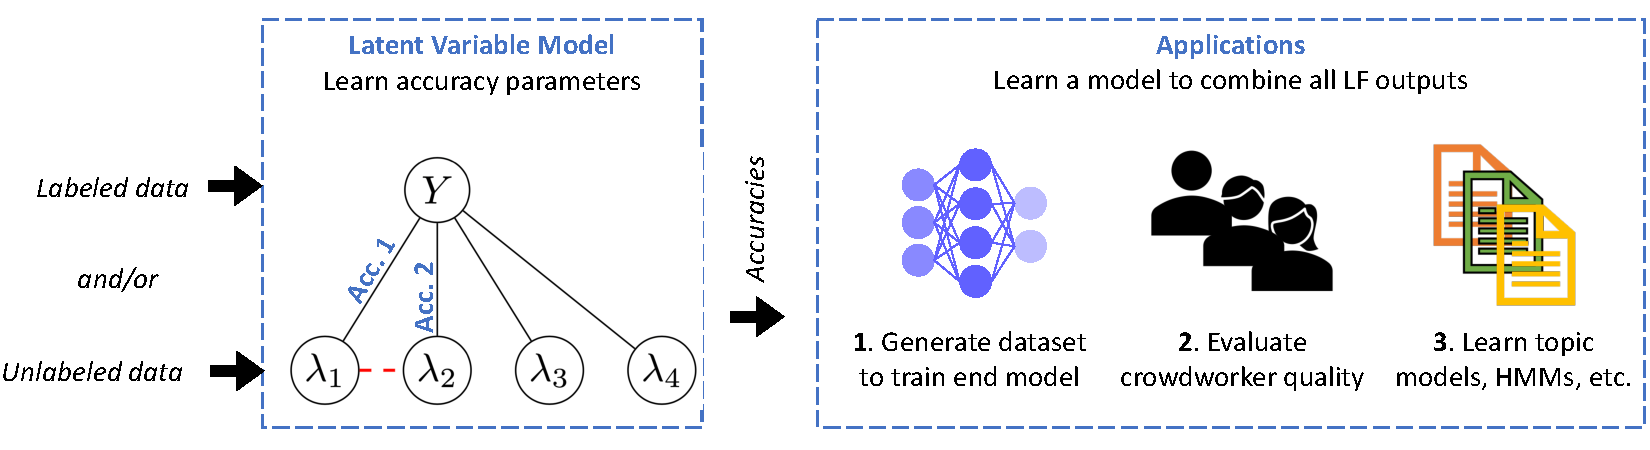
\includegraphics[width=.75\textwidth]{figures/maindiagram.pdf}
    %
    \caption{Latent variable methods (e.g., method-of-moments) can infer an unobserved variable ($Y$) by learning the accuracies of correlated sources ($\lf_1, \ldots, \lf_4$). This is done either from unlabeled data or directly from a small amount of labels; we seek a framework to explain the relative value of these choices. A major challenge are unmodeled dependencies between sources (red). Latent variable models have numerous applications.}
    \label{fig:systemdiagram}
\end{figure*}

Latent variable method-of-moments has been used to learn topic models \citep{anandkumar2014tensor} and parse trees \citep{Hsu12}, to evaluate crowdworkers \citep{joglekar2013evaluating}, and to generate training datasets \citep{Ratner19, fu2020fast}.
In these models, the outputs of sources---variables with some relation to the label---are observed and used to infer the latent variable. The core challenge is to learn the correlations (i.e., \emph{accuracies}) between the sources and the unobserved label variable, which parametrize the model used to generate labels.
%A small amount of labeled data can be used to directly estimate these correlations. 
Here, method-of-moments relies on decomposing multiple observable statistics based on independence among sources. When some labeled data is available, this setup also allows for the accuracy parameters to be directly estimated (\autoref{fig:systemdiagram}).
Therefore, given a limited budget, a principle for choosing between labeled and unlabeled data is crucial, motivating a theoretical framework to understand the relative value between them.

Unmodeled dependencies among sources---a form of model misspecification---are common and yield inconsistent accuracy estimates, which in turn yield poor inferred labels. This affects the value of data produced with latent variable methods, so misspecification must play a role in our framework. While the question of how to analyze misspecification has been studied in classical statistics, the focus is on estimator asymptotics \citep{kleijn2006, kleijn2012}. Our main challenge, however, is to analyze and understand misspecification for both parameter estimation and label inference in the finite---and often small---sample setting.


We theoretically analyze the two alternatives in latent variable methods. In both cases, the output is a joint distribution for the latent variable and observable sources. For the inputs, the choices are either $n_L$ labeled or $n_U$ unlabeled points (and the outputs of $m$ sources). We examine misspecification in the form of unmodeled pairwise dependencies, giving a generalization error analysis for method-of-moments latent variable model performance of the two alternatives. We present a bias-variance decomposition of the generalization error, which for both the labeled and unlabeled data cases consists of (i) irreducible error, (ii) variance, and (iii) bias due to model misspecification at inference time. An important consequence is that for unlabeled data, we incur an additional (iv) standing bias due to incorrectly estimating accuracies that scales with the extent of misspecification, $\mathcal{O}(d/m)$ for $m$ sources and $d$ unmodeled dependencies among them. 

Next, we turn to correcting this standing misspecification bias. In particular, a simple median approach is able to produce consistent estimators given that $d = o(m^2)$ and sufficient amounts of unlabeled data. Therefore, in certain cases, the bias $\mathcal{O}(d/m)$ from misspecification can be completely eliminated. This creates three scenarios to consider for our framework: well-specified (i.e. no unmodeled dependencies), misspecified, and corrected settings, depicted in \autoref{fig:biases}.

We give two applications of our theoretical framework for the three scenarios. First, we develop a criterion, \textit{the data value ratio}, for choosing between labeled and unlabeled data., which is based on the relative minimum amount of labeled points needed to perform as well as a fixed amount of unlabeled points in terms of generalization error. For well-specified models, labeled data is a constant factor more valuable than unlabeled, but for misspecified models the value grows linearly in $d$ and $n_U$. Furthermore, corrected models are able to \emph{improve the value of unlabeled data}. Second, we combine the estimated parameters from the unlabeled approach, which are biased, with ones from the labeled approach---in certain cases outperforming either individually. We validate our framework with synthetic experiments, verify the scaling of our generalization error and data value ratio, and the performance of the combined estimator across the three settings. 

An important real-world application of our results on latent variable methods are weak supervision (WS) frameworks, in particular data programming \citep{Ratner16}, used in a huge range of products and systems across industry and academia. WS frameworks construct datasets without ground-truth annotations by using unlabeled points and distant or weak sources, such as heuristics~\citep{gupta2014improved}, external knowledge bases~\citep{mintz2009distant,craven:ismb99,takamatsu:acl12}, or noisy crowd-sourced labels~\citep{karger2011iterative,dawid1979maximum}. Data programming encompasses many such prior approaches, and has shown excellent results with the method-of-moments approach \citep{fu2020fast}. We perform a real-world WS case study, where ground-truth source dependencies are not known, but sources are likely to be correlated to some extent. We observe that the relative value of labeled data is large, but the value of unlabeled data can be increased via our median approach. With equal amounts of data, the F1-score of a baseline unlabeled approach is 64.81 and the score of a labeled approach is 71.79, but the score of an unlabeled approach with correction is 68.12. This suggests that our theoretical explanation of the effects of misspecification can account for some of the behavior of models on real data.

%A key challenge in data-driven fields is the quality of data. A fixed data collection budget can provide a large amount of noisy or incomplete data, or a smaller but cleaner dataset. Given a choice between these two options, which should we select and which factors should determine this decision? This question, while fundamental, is especially relevant to modern machine learning, where huge datasets are needed to train powerful models. The scale of these models has pushed against the limits of labeling budgets, motivating the use of generative \emph{latent-variable} models that obviate hand-labeling each point.

%Instead, in latent variable methods, the outputs of alternative sources or views---variables that have some relationship to the label---are observed and are used to estimate the value of the latent variable. The core technical challenge is to learn the correlations (i.e., \emph{accuracies}) between the alternative sources and the unobserved label variable. A small amount of labeled data can be used to directly estimate these correlations. They can also be obtained without access to any labels via approaches such as multi-view \emph{latent-variable method-of-moments}---the technique we study in this paper. Both approaches stand to benefit from additional datapoints. Given a limited budget, a principle for choosing between these two is crucial, motivating the need for a theoretical framework to understand the relative value of labeled versus unlabeled data.

%Unmodeled dependencies between these variables---a form of model misspecification---yields inconsistent correlation estimates, producing poor-quality output labels. In turn, this affects the value of data produced with latent variable methods. A principle for choosing between these two is crucial, motivating the need for a theoretical framework to understand the relative value of labeled versus weakly-labeled data.

%We theoretically analyze the two alternatives in latent variable methods. In both cases, the outputs are a set of accuracy parameters, but for the inputs, the choices are either a set of $n_L$ labeled points or a set of $n_U$ unlabeled points and the outputs of $m$ observable sources. We focus on the method-of-moments estimator as our latent-variable method. We examine misspecification in the form of unmodeled pairwise dependencies and incorporate this into a generalization error analysis for latent variable model performance of the two alternatives---the main component of our theoretical framework. We present a bias-variance decomposition of the generalization error, which for both the labeled and unlabeled data cases consists of (i) irreducible error, (ii) variance, and (iii) bias due to model misspecification in statistical inference. An important consequence is that for unlabeled data, we incur an additional (iv) error term due to incorrectly estimating accuracies that scales with the extent of misspecification, $\mathcal{O}(d/m)$ for $m$ sources and $d$ unmodeled dependencies among them. 

%We next turn to correcting this misspecification bias in method-of-moments latent variable estimators. In particular, a simple median approach is able to produce consistent estimators given $d = o(m^2)$ and sufficient amounts of unlabeled data. Therefore, in certain cases, the standing bias $\mathcal{O}(d/m)$ from misspecification can be completely eliminated theoretically. This creates three scenarios to consider our framework in: well-specified (i.e. no unmodeled dependencies), misspecified, and corrected settings, depicted in Figure \ref{fig:biases}.  


%We then present two applications of our theoretical framework for the three scenarios described above. First, we develop a criterion for choosing between labeled and unlabeled data called the \textit{data value ratio}, which is based on the relative minimum amount of labeled points needed to perform as well as a fixed amount of unlabeled points in terms of generalization error. For well-specified models, labeled data is only constant factor more valuable than unlabeled data, but for misspecified models the value grows linearly in the number of dependencies and unlabeled points. Furthermore, corrected (median-based) models are able to \emph{improve the value of unlabeled data}. Second, we discuss how combining the biased parameters learned from the unlabeled dataset with the unbiased ones learned from the labeled dataset can outperform either individually. We validate our theoretical framework with  synthetic experiments, verify the scaling of our generalization error, the scaling of the data value ratio, and the performance of the combined estimator across the three settings. 

%An important real-world application of our results on latent-variable methods are weak supervision (WS) frameworks, in particular data programming \citep{Ratner16}, used in a huge range of products and systems across industry and academia. WS frameworks construct datasets without ground-truth annotations by using unlabeled points and distant or weak sources, such as heuristics~\citep{gupta2014improved}, external knowledge bases~\citep{mintz2009distant,craven:ismb99,takamatsu:acl12}, or noisy crowd-sourced labels~\citep{karger2011iterative,dawid1979maximum}. Data programming encompasses many such prior approaches, and has shown excellent results with the method-of-moments approach \citep{fu2020fast}. We perform real-world weak supervision experiments, where ground-truth source dependencies are not known, but sources are likely to be highly correlated. In several cases, we observe that the relative value of labeled data is large, but can be reduced via our median approach. \todo{Number here}. This suggests that our theoretical explanation of the effects of misspecification can account for some of the behavior of models on real data.



%, so misspecification must be theoretically factored into our framework. While the question of how to analyze misspecification has been studied in classical statistical works, they primarily focus on asymptotic behavior of estimators~\citep{kleijn2006, kleijn2012}. Our main challenge, however, is to handle the finite---and often very small---sample setting since we wish to compare datasets practically. 


%Given a choice between these two options, which should we select and which factors should determine this decision? This question, while fundamental, is especially relevant to an important area of machine learning---weakly-supervised learning---where such datasets are used to train an intermediate model that outputs a larger, de-noised dataset to be used downstream (e.g., to train a data-hungry deep model).
%


%Why is it interesting and important?
%Such techniques are motivated by the scale of modern ML, which has pushed against the limits of budgets for building hand-labeled datasets. Weak supervision (WS) frameworks, in particular data programming \citep{Ratner16}---used in a huge range of products and systems across industry and academia---construct datasets without ground-truth annotations by using unlabeled points and distant or weak sources, such as heuristics~\citep{gupta2014improved}, external knowledge bases~\citep{mintz2009distant,craven:ismb99,takamatsu:acl12}, or noisy crowd-sourced labels~\citep{karger2011iterative,dawid1979maximum}. Data programming encompasses many approaches and has the advantage of being expressed in terms of classical models, allowing for theoretical analysis. Such approaches benefit from adding more labeled data and/or  \textit{weakly-labeled} data, i.e., unlabeled points in the context of weak sources. A principle for choosing between these two is crucial, motivating the need for a theoretical framework to understand the relative value of labeled versus weakly-labeled data.

% Why is it hard? (E.g., why do naive approaches fail?)



%The core technical challenge in WS is to learn the accuracies of weakly-labeled data sources. A latent variable statistical model whose parameters include the accuracies is fit to the weakly-labeled data and then used to output de-noised labels on the data. Unmodeled dependencies between sources---a form of model misspecification---yields inconsistent source accuracy estimates, producing poor-quality output labels. In turn, this affects the value of weakly-labeled data, so misspecification must be theoretically factored into our framework. While the question of how to analyze misspecification has been studied in classical statistical works, they primarily focus on asymptotic behavior of estimators~\citep{kleijn2006, kleijn2012}. Our main challenge, however, is to handle the finite---and often very small---sample setting since we wish to compare datasets practically. 

%We theoretically analyze the two alternatives in weak supervision pipelines. In both cases, the outputs are a set of accuracy parameters, but for the inputs, the choices are either a set of $n_L$ labeled points or a set of $n_U$ weakly-labeled points from $m$ weak sources. We examine misspecification in the form of unmodeled pairwise dependencies and incorporate this into a generalization error analysis for WS model performance of the two alternatives---the main component of our theoretical framework. We present a bias-variance decomposition of the generalization error, which for both the labeled and weakly-labeled data cases consists of (i) irreducible error, (ii) variance, and (iii) bias due to model misspecification in statistical inference. An important consequence is that for weakly-labeled data, we incur an additional (iv) error term due to incorrectly estimating accuracies that scales with the extent of misspecification, $\mathcal{O}(d/m)$ for $m$ sources and $d$ unmodeled dependencies among them. 



%We next turn to correcting this misspecification bias. In particular, a simple median approach is able to produce consistent estimators given $d = o(m^2)$ and sufficient amounts of weakly-labeled data, and this finding also broadly applies to other method-of-moments algorithms that exploit multiple, conditionally-independent views of latent variables. Therefore, the standing bias $\mathcal{O}(d/m)$ from misspecification can be completely eliminated theoretically. This creates three scenarios to consider our framework in: well-specified (i.e. no unmodeled dependencies), misspecified, and corrected settings, depicted in Figure \ref{fig:biases}.  

%We then present two applications of our theoretical framework for the three scenarios described above. First, we develop a criterion for choosing between labeled and weakly labeled data called the \textit{data value ratio}, which is based on the relative minimum amount of labeled points needed to perform as well as a fixed amount of unlabeled points in terms of generalization error. For well-specified models, labeled data is only constant factor more valuable than unlabeled data, but for misspecified models the value grows linearly in the number of dependencies and unlabeled points. Furthermore, corrected (median-based) models are able to \emph{reduce the value of labeled data}. Second, we discuss how combining the biased parameters learned from the unlabeled dataset with the unbiased ones learned from the labeled dataset can outperform either individually.

%What are the key components of my approach and results? Also include any specific limitations.
%We validate our theoretical framework with  synthetic experiments, verify the scaling of our generalization error, the scaling of the data value ratio, and the performance of the combined estimator across the three settings. In addition, we collect real-world experimental data, where ground-truth dependencies are not known, but sources are likely to be highly correlated. In several cases, we observe that the relative value of labeled data is large, but can be reduced via our median approach. This suggests that our theoretical explanation of the effects of misspecification can account for some of the behavior of models on real data.



%%%%%%%%%%%%%%%%%%%%%%%%%%%%%%%%% OLD (10/14)


%A key challenge in data-driven fields is the quality
%of training data. A fixed data collection budget can
%provide a large amount of noisy or incomplete training data, or a smaller but cleaner dataset. Given a
%choice between these two options, which should we
%select and which factors should determine this decision? This question, while fundamental, is especially
%relevant to an important area of machine learning—
%weakly-supervised learning—where such datasets are
%used to train an intermediate model that outputs a
%larger, de-noised dataset to be used downstream (e.g.,
%to train a data-hungry deep model).

%Such techniques are motivated by the scale of modern ML, which has pushed against the limits of budgets for building hand-labeled datasets. Weak supervision (WS) frameworks, in particular data programming (Ratner et al., 2016)—used in a huge range of
%products and systems across industry and academia—
%construct datasets without ground-truth annotations
%by using unlabeled points and distant or weak sources,
%such as heuristics (Gupta and Manning, 2014), external knowledge bases (Mintz et al., 2009; Craven
%and Kumlien, 1999; Takamatsu et al., 2012), or noisy
%crowd-sourced labels (Karger et al., 2011; Dawid and
%Skene, 1979). Data programming encompasses many
%approaches and has the advantage of being expressed
%in terms of classical models, allowing for theoretical
%analysis. Such approaches benefit from adding more
%labeled data and/or weakly-labeled data, i.e., unlabeled
%points in the context of weak sources. A principle for
%choosing between these two is crucial, motivating the
%need for a theoretical framework to understand the
%relative value of labeled versus weakly-labeled data.


%The core technical challenge in WS is to learn the accuracies of weakly-labeled data sources. A latent variable statistical model whose parameters include the
%accuracies is fit to the weakly-labeled data and then
%used to output de-noised labels on the data. Unmodeled dependencies between sources—a form of model
%misspecification—yields inconsistent source accuracy
%estimates, producing poor-quality output labels. In
%turn, this affects the value of weakly-labeled data, so
%misspecification must be theoretically factored into our
%framework. While the question of how to analyze misspecification has been studied in classical statistical
%works, they primarily focus on asymptotic behavior
%of estimators (Kleijn and van der Vaart, 2006, 2012).
%Our main challenge, however, is to handle the finite—
%and often very small—sample setting since we wish to
%compare datasets practically.


%We theoretically analyze the two alternatives in weak
%supervision pipelines. In both cases, the outputs are
%a set of accuracy parameters, but for the inputs, the
%choices are either a set of $n_L$ labeled points or a set of
%$n_U$ weakly-labeled points from m weak sources. We
%examine misspecification in the form of unmodeled
%pairwise dependencies and incorporate this into a gen-
%eralization error analysis for WS model performance
%of the two alternatives—the main component of our
%theoretical framework. We present a bias-variance de-
%composition of the generalization error, which for both
%the labeled and weakly-labeled data cases consists of
%(i) irreducible error, (ii) variance, and (iii) bias due to
%model misspecification in statistical inference. An im-
%portant consequence is that for weakly-labeled data,
%we incur an additional (iv) error term due to incor-
%rectly estimating accuracies that scales with the ex-
%tent of misspecification, $\mathcal{O}(d/m)$ for $m$ sources and $d$
%unmodeled dependencies among them.
%We next turn to correcting this misspecification
%bias. In particular, a simple median approach is
%able to produce consistent estimators given $d = o(m^2)$ and sufficient amounts of weakly-labeled data,
%and this finding also broadly applies to other
%method-of-moments algorithms that exploit multiple,
%conditionally-independent views of latent variables.
%Therefore, the standing bias $\mathcal{O}(d/m)$ from misspecification can be completely eliminated theoretically.
%This creates three scenarios to consider our framework
%in: well-specified (i.e. no unmodeled dependencies),
%misspecified, and corrected settings, depicted in Fig-ure 1.


%We then present two applications of our theoretical
%framework for the three scenarios described above.
%First, we develop a criterion for choosing between la-
%beled and weakly labeled data called the data value
%ratio, which is based on the relative minimum amount
%of labeled points needed to perform as well as a fixed
%amount of unlabeled points in terms of generalization
%error. For well-specified models, labeled data is only
%constant factor more valuable than unlabeled data, but
%for misspecified models the value grows linearly in the
%number of dependencies and unlabeled points. Furthermore, corrected (median-based) models are able
%to reduce the value of labeled data. Second, we discuss
%how combining the biased parameters learned from the
%unlabeled dataset with the unbiased ones learned from
%the labeled dataset can outperform either individually.
%We validate our theoretical framework with synthetic
%experiments, verify the scaling of our generalization error, the scaling of the data value ratio, and the performance of the combined estimator across the three set-
%tings. In addition, we collect real-world experimental
%data, where ground-truth dependencies are not known,
%but sources are likely to be highly correlated. In several cases, we observe that the relative value of labeled
%data is large, but can be reduced via our median approach. This suggests that our theoretical explanation
%of the effects of misspecification can account for some
%of the behavior of models on real data.
 \section{Related Work}
 \vspace{-.5em}
%\paragraph{Method-of-Moments Estimators}
%A tranche of latent variable model literature relies on the method-of-moments approach. These estimation approaches 
%often involve decomposing multiple observable ``views'' of latent variables. The decomposition is applied to closed-form systems of equations~\citep{joglekar2013evaluating, fu2020fast} and tensors~\citep{anandkumar2014tensor, chaganty2014estimating, Bhaskara14}, but in all cases, conditional independence among the views is required for the structural relationships to hold. We focus on a particular approach in this paper, but our analysis can provide error decomposition under misspecification for other method-of-moments estimators.

\vspace{-0.5em}
\paragraph{Misspecification in Graphical Models}
The asymptotic effect of misspecification on parameter estimation is studied by \cite{kleijn2012}, extending the Bernstein-Von Mises theorem to cases where observed samples are not of the parametric distribution being estimated. %They find that certain estimators, such as MLE, converge to a normal distribution centered at the point that results in a parametrized distribution closest in Kullback-Leibler divergence to the true distribution, and this property is directly used in asymptotic analysis of estimators in Bayesian and variational inference \cite{wang2019variational, hongmartin2020}. 
However, their main results do not fully extend to method-of-moments estimators. Other analyses of model misspecification directly examine families of models, such as \cite{JogL15}'s lower bound on KL-separation of Gaussian graphical models. While this bound is important for modeling errors in inference,
%a version of their mutual information bounds appear as an inference bias in our error analysis, 
it does not illustrate our additional error in parameter estimation. More generally, works on misspecification either study a particular class of techniques~\citep{Blasi13} or a particular model and propose repairs~\citep{Grunwald17}---while we compare effects on alternative datasets.

\vspace{-0.5em}
\paragraph{Structure Learning}
One way to reduce misspecification is to produce a more refined model. Graphical model structure learning aims to do so in both the supervised~\citep{Ravikumar11, Loh13} and unsupervised cases~\citep{Chandrasekaran12,Meng14, bach2017learning, varma2019learning}. However, these works present computational challenges, require (often strong) conditions to hold, and do not analyze the downstream impact of errors. Our approach instead focuses on understanding the impact of errors and is applicable to partial recovery that often results from structure learning.

%\paragraph{Semi-Supervised Learning} involves using a small set of labeled points and a larger set of unlabeled points~\citep{Chapelle09, zhu2009introduction}. There are a wide variety of such techniques: the missing labels can be modeled as latent variables and expectation maximization (EM) can be used~\citep{Nigam2000}. Another approach uses a graph structure to propagate labels, relying on MRFs~\citep{Zhu02} or kernels~\citep{Kondor02}. In contrast to such techniques, WS can operate with no labels. It does not focus on extending any given labels, but rather learning the weak sources that can be applied to any data. 

%does not require any labels, and by learning the accuracies of sources that can then be applied to any unlabeled data


%\todo{maybe data shapley or stuff like that?}
%There has also been recent work in data valuation \citep{ghorbani2019data}, but they focus on a per-point valuation for a fixed supervision setting rather than a comparison between labeled and unlabeled data approaches. 
\section{Background and Problem Setting} \label{sec:background}
\vspace{-.5em}
We start with background on latent variable models and introduce the model we analyze. We explain the stages---learning accuracies and inferring labels---for both the labeled and unlabeled cases, and conclude with model evaluation and key challenges.

\begin{figure*}
    \centering
    \hspace*{-.5cm}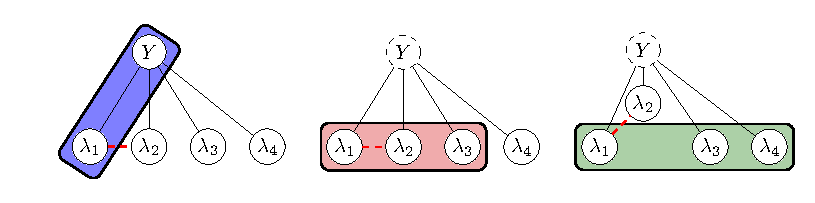
\includegraphics[width=.7\textwidth]{figures/models.pdf}
    % \hspace*{-.6cm}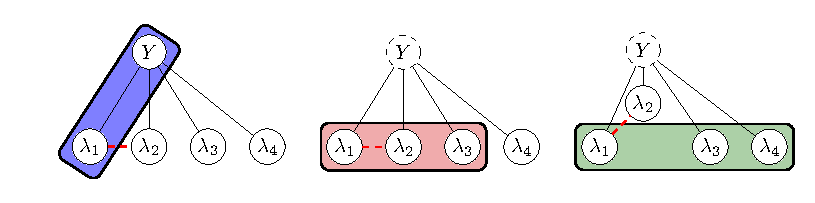
\includegraphics[width=.525\textwidth]{figures/models.pdf}
    %
    \caption{Latent variable models with unmodeled dependency (red edge), leading to misspecification. Boxes indicate observable variables used for accuracy estimation. Left: model with access to label $Y$. Pairs $(\lambda_i, Y)$ directly estimate source accuracy. Center: latent model with unobserved $Y$. Triplet (red) includes unmodeled dependency, leading to inconsistent estimation. Right: Corrected model using medians. Triplet excludes the dependency, returning to consistency.}
    \label{fig:biases}
\end{figure*}

%In this section, we provide background on the weak supervision problem setting, the graphical model assumptions for the true distribution as well as the misspecified model used, and the method-of-moments approach commonly used to learn model parameters when labeled data is unavailable.  

%This work explores when and how a small number of labeled data points can be used to improve the quality of noisy labels produced by the data programming pipeline. In Section \ref{sec:setting_dp} we provide background about data programming and methods for combining labeling functions. In Section \ref{sec:setting_adding_labels} we describe the modified setting where some labeled data is available. Finally, we discuss evaluating data programming methods in Section \ref{sec:setting_evaluation}.

%\subsection{Background: Data Programming}
%\label{sec:setting_dp}

\paragraph{Setup} In latent variable models, a number of sources are observed and used to infer the latent variable.
%In weak supervision frameworks, e.g., data programming \citep{Ratner16}, a labeled dataset is built by acquiring noisy sources operating on unlabeled data. %The outputs of these sources %. Often a programmatic heuristic written by practitioners, each weak source either votes or abstains on a data point, thus overall producing multiple noisy labels per point that are then
%are aggregated by a \emph{label model} to output the training label for each point. 
The input is usually $n_U$ unlabeled data points, but in our setting we also consider a small \emph{labeled} dataset of $n_L$ samples. The output is a large, labeled dataset.

Let $X \in \X$ and $Y \in \mathcal{Y} = \{-1, 1\}$. We consider an unlabeled dataset $\bm{X}_U = \{x_i^U\}_{i = 1}^{n_U}$ and a labeled dataset $(\bm{X}_L, \bm{Y}_L) = \{(x_i^L, y_i^L) \}_{i = 1}^{n_L}$ drawn from the distribution of $(X, Y)$.
There are $m$ sources, each
outputting a value in $\{-1, +1\}$ via a deterministic function
%on $X$ via a deterministic \textit{labeling function} (LF)
$\lf_j: \X \rightarrow \mathcal{Y}$ for all
$j \in [m]$. % ($\lf_j(X) = 0$ is an abstain). 
Our goal is to use the outputs of $\bm{\lf}$, the vector of sources, to construct a model to infer $Y$.

To infer $Y$, we learn the model $\Pr(Y, \bm{\lf})$ and then marginalize to produce soft labels $\widetilde{y}_i := 2 \Pr(Y = 1 | \bm{\lf} = \bm{\lf}(x_i)) - 1 \in [-1, 1]$ for each $x_i$ by applying
the $m$ sources to $\bm{X}_U$ and $(\bm{X}_L, \bm{Y}_L)$. The overall approach has two steps: (i) learn the latent variable model (using labeled or unlabeled data), and (ii) infer labels $\tilde{y}_i$.

%We use the label model outputs as the final predictions for $Y$ such that its generalization error precisely captures the effect of model misspecification and labeled versus unlabeled data. However, the labels are often used to train an additional end model, for which our analysis on the quality of training data is still valid.

% \paragraph{Misspecification in weak supervision}
% To learn the joint distribution $\Pr(Y,\bm{\lf})$, we typically assume that there exist subsets of labeling functions that are conditionally independent given $Y$. When 

\paragraph{Theoretical model}
We pick a simple model that captures many latent variable model settings and still presents all of the challenges for comparing between the types of data. We assume an Ising model for $\Pr(Y, \bm{\lf})$; the only difference between the labeled and unlabeled setting is that $Y$ is latent in the latter. %Following the standard notation,
%We present the standard graphical model assumptions for the true distribution $\Pr(Y, \bm{\lf})$. Then, we discuss the misspecified graphical model used in weak supervision and how it outputs labels.
The set of canonical parameters is $\Theta$, and the dependency graph is $G = (V, E)$, where $V = Y \cup \bm{\lf}$ and $E$ consists of edges from $Y$ to the sources as well as the $d$ edges among the sources, $E_{\lf}$. %The graph $G$ specifies dependencies using standard technical notions from the PGM literature~\citep{koller2009probabilistic, Lauritzen, wainwright2008graphical}. 
The lack of an edge in $G$ between a pair of
variables indicates independence conditioned on a separator set~\citep{Lauritzen}, so the true distribution can be modeled as
\begin{align}
    \Pr(Y, \bm{\lf}) = \frac{1}{Z} \exp \Big(\theta_Y + \sum_{i = 1}^m \theta_i \lf_i Y + \sum_{(i, j) \in E_{\lf}} \theta_{ij} \lf_i \lf_j \Big),
    \label{eq:true_pgm} \nonumber 
    \vspace{-0.5em}
\end{align}
with cumulant function $Z$. For cleaner presentation, we assume $\Theta \ge 0$ (no sources that disagree with others or $Y$ on average) and $E_{\lf}$ is sparse enough such that $\text{deg}(\lf_i) \le 2$ for all $\lf_i$ (each source is conditionally dependent on at most one other source). This leads to model misspecification when edges are unknown.

%With this, we can explain the two steps involved in the process.

\paragraph{Inference} The label is computed using a naive Bayes approach that assumes all sources are conditionally independent with $E_{\lf} = \emptyset$:
\begin{align}
    \widetilde{\Pr}(Y &= 1 | \lf = \lf(X)) \nonumber \\
    &= \frac{\prod_{i = 1}^m \widetilde{\Pr}(\lf_i = \lf_i(X) | Y = 1) \Pr(Y = 1)}{\hat{\Pr}(\lf = \lf(X))} 
    \label{eq:inference}
\end{align}
where the class balance $\Pr(Y = 1)$ is assumed to be known, $\hat{\Pr}$ is an empirical probability
, and $\widetilde{\Pr}$ indicates an estimated probability resulting from the parameter estimation step described below. %The class balance $\Pr(Y = 1)$ is assumed to be known, so the only term to be estimated is $\widetilde{\Pr}(\lf_i = \lf_i(X) | Y = 1)$ for each $\lf_i$, which we describe how to do below. 
%
In practice, the conditional independence assumptions required for (\ref{eq:inference}) may not hold, but dependencies among sources are often unknown%\footnote{We discuss techniques to rectify this and their costs at the end of the following section.}
. Therefore, conditional independence is assumed, and we may suffer from \emph{misspecification} in inferring our probabilistic labels. %In the following we compute the cost of this error and its implications for the value of data. 

%Note that in the case of labeled data, we can compute this directly, but for unlabeled data, we estimate this probability using the graphical model structure.

\paragraph{Learning parameters with method-of-moments}
For the labeled dataset, we estimate $\widetilde{\Pr}(\lf_i = \lf_i(X) | Y = 1)$ in (\ref{eq:inference}) directly from samples, as $Y$ is observed. 

For the unlabeled dataset, we use the method-of-moments estimator from \cite{fu2020fast}, which relies on the property
%\begin{proposition} 
that if $\lf_i \independent \lf_j | Y$, then $\lf_i Y \independent \lf_j Y$.
%\label{prop:triplet}
%\end{proposition}
%
This implies that $\E{}{\lf_i Y} \cdot \E{}{\lf_j Y} = \E{}{\lf_i \lf_j Y^2} = \E{}{\lf_i \lf_j},$ which is directly estimable.
Define $a_i := \E{}{\lf_i Y}$ as the unknown \textit{accuracy} of $\lf_i$. If we can introduce a third $\lf_k$ that is conditionally independent of $\lf_i$ and $\lf_j$, we have a system of equations that can be solved using observable statistics. We use this \textit{triplet method} to recover these accuracies: we choose two $\lf_j$, $\lf_k$ at random for each $\lf_i$ and solve up to sign:
\begin{align}
    |\widetilde{a}_i^{(j, k)}| := \sqrt{\bigg| \frac{\Ehat{\lf_i \lf_j} \Ehat{\lf_i \lf_k}}{\Ehat{\lf_j \lf_k}} \bigg|},
    \label{eq:triplet}
\end{align}
where $\hat{\mathbb{E}}$ is an empirical estimate of the expectation. %using the weakly labeled dataset $\bm{X}_U$. 
We use the estimated $\widetilde{a}_i^U := \widetilde{a}_i^{(j, k)}$ to directly compute $\widetilde{\Pr}(\lf_i = \pm 1 | Y = 1)$ for \eqref{eq:inference}. However, random $\lf_j$ and $\lf_k$ may not satisfy conditional independence, and thus we incur error in estimating accuracies due to misspecification in a way unique to the unlabeled setting. We aim to capture this error in our evaluation. % The following section characterizes this notion.

\paragraph{Evaluating the model}
We define the model's generalization error as $R = \mathbb{E}_{(Y, \bm{\lf}), \N, \tau}[l(\widetilde{Y}, Y)]$ where expectation is taken over the distribution of $(Y, \bm{\lf})$, $\N$ (the random dataset used), and $\tau$ (the algorithmic randomness, i.e. the triplets used in method-of-moments). $l(\cdot, \cdot)$ here is the cross entropy loss,
%\steve{maybe move this up to the beginning of the paragraph, so the ordering is more natural?}  defined on a point $(x_i, y_i)$ as
$l(\widetilde{y}_i, y_i) = -\frac{1 + y_i}{2} \log \widetilde{\Pr}(Y = 1 | \lf = \lf(x_i))
- \frac{1 - y_i}{2} \log \widetilde{\Pr}(Y = -1 | \lf = \lf(x_i)).$
Let $R_U$ denote the error for the unlabeled dataset and $R_L$ for labeled.

% \paragraph{Key Technical Challenges}
% The goal of our evaluation framework is to answer questions such as
% \begin{itemize}
%   \setlength\itemsep{0em}
%     \item The weakly labeled case computes the function (\ref{eq:triplet}) of empirically observable quantities, while the labeled case accesses them directly---how do the errors due to sampling noise compare? 
%     \item Which stage of the pipeline---learning the model and inference---does misspecification impact, and how does this differ between the cases?
%     %\item How to price $n_L$ labeled samples in terms of the cheaper weakly labeled ``currency''?
% \end{itemize}


%%%%%%%%%%%%%%%%%%%%%%%%%%%%%%%%%%%%%%%%%%%%%%%%%%%%%%%%%%%%%%%%%%%%%%%%%%%%%%%%%%%%%%%%%%



%We define the data programming task for binary classification as follows. Let $X\in\mathcal{X}$ for some set $\mathcal{X}$ of possible inputs and $Y\in\{-1,1\}$ where $(X,Y)\sim\mathcal{D}$ for some distribution $\mathcal{D}$. We are given an unlabeled dataset $\boldsymbol{X}_U=\{x^i_U\}_{i=1}^{n_U}$ with corresponding unobserved gold labels $\boldsymbol{Y}_U=\{y^i_U\}_{i=1}^{n_U}$ where $(x^i_U,y^i_U)$ are i.i.d. samples from $\mathcal{D}$. We are also given $m$ labeling functions $\lambda_1,\hdots,\lambda_m$ where $\lambda_j:\mathcal{X}\to\{-1,0,1\}$ with an output of $0$ denoting that the labeling function \textit{abstains} (does not provide an answer). We say that a labeling function \textit{fires} when it does provide an answer. Labeling functions are typically fairly accurate but only fire on a small fraction of points. Our goal is to use our $m$ labeling functions to produce noisy labels $\tilde{\boldsymbol{Y}}=\{\tilde{y}^i\}_{i=1}^{n_U}$ with $\tilde{y}^i\in[-1,1]$ representing our confidence about the gold label (for example, the probabilistic label might be closer to $0$ if labeling functions disagree). These noisy labels can then be used as training data.


%Aggregating labeling function outputs usually involves estimating the \textit{accuracy} and \textit{coverage} of each labeling function from \textit{only unlabeled data} and then weighting labeling functions according to these two parameters. The accuracy $\alpha_j$ of the $j$'th labeling function is the accuracy over the points where it fires and the coverage $\beta_j$ of the $j$'th labeling function is the fraction of points where it fires.
%\begin{equation}
%\alpha_j=\text{Pr}[\lambda_j(X)=Y\mid\lvert\lambda_j(X)\rvert=1]
%   \quad\text{and}\quad 
%\beta_j=\text{Pr}[\lvert\lambda_j(X)\rvert=1]
%\end{equation}
%Several methods have been proposed for estimating accuracies and coverages, including marginal maximum likelihood estimation, completing the covariance matrix between labeling function outputs and the unobserved true labels, and solving for the accuracies of three labeling functions (for which a closed-form solution exists) at a time \citep{alex2016data, ratner2019training, fu2020fast}. While estimating coverages from unlabeled data is easy, estimating labeling function accuracies requires making assumptions about their behavior. Most previous methods assume that labeling functions are conditionally independent given the gold label, that is
%\begin{equation}
%    \text{Pr}[\lambda(X)=\boldsymbol{z}\mid Y=y]=\prod_{j=1}^m\text{Pr}[\lambda_j(X)=z_j\mid Y=y]
%\end{equation}
%Efforts have been made to learn dependencies between labeling functions \citep{bach2017learning, varma2019learning} and previous data programming methods propose model variants which permit dependencies, but they ultimately rely on subsets of conditionally independent labeling functions to estimate accuracies. Furthermore, models which assume that all labeling functions are conditionally independent, such as the base model from \cite{Ratner_2017}, are in practice often used out-of-the-box. Therefore, in this work we study data programming models which assume that all labeling functions are conditionally independent.

%\subsection{Adding labeled data to the data programming setup}
%\label{sec:setting_adding_labels}

%For this work, we modify the standard data programming setup such that in addition to labeling functions the expert provides a small number of labeled data points. Our task is the same as above, except that we are also given a labeled dataset $\boldsymbol{X}_L=\{x^i_L\}_{i=1}^{n_L}$ with observed gold labels $\boldsymbol{Y}_L=\{y^i_L\}_{i=1}^{n_L}$ where again $(x^i_L,y^i_L)$ are i.i.d. samples from $\mathcal{D}$. We are interested in settings where the labeled dataset size $n_L$ is much smaller than the unlabeled dataset size $n_U$ because if $n_L$ is close to $n_U$ supervised or semi-supervised approaches would likely perform well and data programming would not be necessary.

%\subsection{Evaluating noisy labels directly}
%\label{sec:setting_evaluation}

%Generally in data programming the quality of the noisy training labels is measured by training an \textit{end model} on these labels and evaluating its performance on a test set. Because the end model performance is dependent on the choice of architecture and generally correlates with the quality of the noisy labels, we instead directly measure the accuracy of the noisy labels. In our modified setting, the labels $\boldsymbol{Y}_L$ are given for the subset $\boldsymbol{X}_L$ of the training data so we evaluate noisy labels produced for an unseen test set. We define accuracy of noisy labels $\tilde{\boldsymbol{Y}}_\text{test}=\{\tilde{y}_\text{test}^i\}_{i=1}^{n_\text{test}}$ where $\tilde{y}_\text{test}^i\in[-1,1]$ with true test labels $\boldsymbol{Y}_\text{test}=\{y_\text{test}^i\}_{i=1}^{n_\text{test}}$ where $y_\text{test}^i=\{-1,1\}$ as follows (with predictions of $0$ considered ``half'' correct).
%\begin{equation}
%    A(\boldsymbol{Y}_\text{test},\tilde{\boldsymbol{Y}}_\text{test})=\frac{1}{n_\text{test}}\sum_{i=1}^{n_\text{test}}\begin{cases}
%        1&\text{ if }\text{sign}(\tilde{y}_\text{test}^i)=y_\text{test}^i\\
%        1/2&\text{ if }\tilde{y}_\text{test}^i=0\\
%        0&\text{ otherwise}
%    \end{cases}
%\end{equation}


\section{Theoretical Results} \label{sec:theory}
\vspace{-.5em}
We theoretically analyze the quality of the latent variable model, taking into account the impact of misspecification when using unlabeled versus labeled data. %The results produce a practical criterion for valuing supervision. %First, we discuss the error in the labeling functions' accuracy parameters $a_i$ for both the labeled and unlabeled data case. 
%Then, we propagate this error into our computation of the 
In \ref{subsec:decomp} we give 
%bounds the accuracy estimation error that arises from using unlabeled data under misspecification. Next, we use these to present
an exact decomposition of the generalization error of the latent variable model, which demonstrates how misspecification is present in both the parameter learning and inference steps of the model when data is unlabeled and only present in the latter when data is labeled. In \ref{subsec:scaling}, we bound the generalization error using this framework to show how the unlabeled case has an additional standing bias of $\mathcal{O}(d/m)$. Given this standing bias, in \ref{sec:misspec}, we introduce a simple method that under certain conditions can correct for dependency-based misspecification. We analyze this correction's impact on generalization error. 



% misspecification impacts parameter estimation only when the data is unlabeled; therefore, this particular term is crucial in determining which dataset has lower generalization error. We then discuss ways to mitigate misspecification's impact on parameter estimation. Lastly, using our error analysis we propose our data value criterion for choosing between and combining unlabeled and labeled data.
%and present upper and lower bounds on the generalization error of our label model, again for both labeled and unlabeled data cases separately. In each part, we contrast the labeled and unlabeled data settings. Lastly, we use these bounds to propose a data value criterion.

\subsection{Decomposition Framework}
\label{subsec:decomp}%for WS Label Model}
\vspace{-0.5em}

%We define the generalization error as $\mathbb{E}[l(\widetilde{Y}, Y)]$, where 
%\begin{align*}
%&l(\widetilde{y}_i, y_i) = -\left(\frac{1 + y_i}{2}\right) \log \widetilde{\Pr}(Y = 1 | \lf = \lf(x_i)) \\
%&- \left(\frac{1 - y_i}{2}\right) \log \widetilde{\Pr}(Y = -1 | \lf = \lf(x_i))
%\end{align*} is the cross-entropy loss on a point $(x_i, y_i)$. The expectation is taken over $(Y, \bm{\lf})$, the random triplets chosen to estimate each $a_i$, and the finite samples used. 

%One immediate consequence of model misspecification in the case of unlabeled data is that the  $\lf_i, \lf_j, \lf_k$ used to estimate $a_i$ may not be pairwise conditionally independent. This results in biased (and inconsistent) estimation when data is unlabeled. In contrast, in the labeled data setting, the $a_i$'s can be directly estimated as $\Ehat{\lf_i Y}$.

%\begin{lemma}[Accuracy Bias] 
%Suppose each $a_i$ is estimated by randomly choosing $\lf_j$ and $\lf_k$ in \eqref{eq:triplet} in the case of unlabeled data, and let $a_{\min} = \min_i a_i$ and $b_{\min} = \min_{i, j} \E{}{\lf_i \lf_j}$. Assume that the true distribution satisfies \eqref{eq:true_pgm} with $|E_{\lf}| = d$ and that $a_{\min} b_{\min} \ge \frac{d - 1}{m - 2}$. Then the expectation of the asymptotic bias of $\widetilde{a}^U$, which we refer to as $\bar{a}$, is 
%\begin{align}
%     \frac{d \varepsilon_{\min}}{m - 1} \left( \frac{(m - 2d) b_{\min}^2}{m - 2} \right)\le  \|\E{}{\widetilde{a}^U} - a\|_1 \le \frac{d \varepsilon_{\max}}{m - 1} \left(\frac{2}{b_{\min} a_{\min}} + \frac{1}{b_{\min}^2 a_{\min}^2} \right),
%\end{align}

%$\varepsilon_{\max}$ is an upper bound on $\varepsilon_{ij} = \E{}{\lf_i \lf_j} - \E{}{\lf_i Y} \E{}{\lf_j Y}$ for all $(i, j) \in E_{\lf}$, and $\varepsilon_{\min} \ge 0$ is a lower bound. In particular, $\varepsilon_{ij} = \frac{8}{Z_{ij}} \sinh(\theta_{ij})(\cosh(2\theta_i) + \cosh(2\theta_j) - \frac{64}{Z_{ij}^2} \sinh^2(\theta_{ij}) \sinh(2\theta_i) \sinh(2\theta_j)$ where $Z_{ij}$ is a product of marginal cumulant functions.  
%\label{lemma:accuracy_bias}
%\end{lemma}

%From this result, we see that when $d = 0$, $\E{}{\widetilde{a}^U} = \E{}{\widetilde{a}^L} = a$, meaning that the asymptotic estimator is unbiased. However, as the number of dependencies or the strength of the correlation $\theta_{ij}$ relative to $\theta_i$ and $\theta_j$ increases, there is a standing bias, and it worsens. \todo{where should I put assumptions used for these theorems? i.e. $\theta_i, \theta_j, \theta_{ij} \ge 0$ for this analysis}

%\paragraph{Bounding the generalization error}

%The estimation error for $\widetilde{a}_i^U$ is now propagated into the generalization error for the label model. We define the generalization error as $\mathbb{E}[l(\widetilde{Y}, Y)]$, where \[l(\widetilde{y}_i, y_i) = -\left(\frac{1 + y_i}{2}\right) \log \widetilde{\Pr}(Y = 1 | \lf = \lf(x_i)) - \left(\frac{1 - y_i}{2}\right) \log \widetilde{\Pr}(Y = -1 | \lf = \lf(x_i))\] is the cross-entropy loss. The expectation is taken over $(Y, \bm{\lf})$, the random triplets chosen to estimate each $a_i$, and the finite samples used. 

Our first result is a decomposition of the generalization error into four components. The last two components, the inference bias and parameter estimation error, reflect the role of misspecification.
\begin{theorem}
The generalization error has the following decomposition:
\ifsinglecolumn
\begin{align}
    &\E{}{l(\widetilde{Y}, Y)} = \underbrace{H(Y | \bm{\lf})}_{{\mathrm{Irreducible \; error}}} - \underbrace{\E{\N}{\KL(\Pr(\bm{\lf}) || \hat{\Pr}(\bm{\lf}))}}_{\mathrm{Observable \; sampling \; noise}} + \sum_{{(i, j) \in E_{\lf}}} \underbrace{I(\lf_i; \lf_j | Y)}_{\mathrm{Inference \; bias}} +  \sum_{i = 1}^m \underbrace{\E{Y, \N, \tau}{\KL(\mathrm{Pr}_{\lf_i | Y} || \widetilde{\Pr}_{\lf_i | Y })}}_{\mathrm{Parameter \;estimation \;error}} \nonumber,
\end{align}
\else 
\begin{align}
    &\E{}{l(\widetilde{Y}, Y)} = \underbrace{H(Y | \bm{\lf})}_{\mathclap{\mathrm{Irreducible \; error}}} - \underbrace{\E{\N}{\KL(\Pr(\bm{\lf}) || \hat{\Pr}(\bm{\lf}))}}_{\mathrm{Observable \; sampling \; noise}} + \nonumber \\ %\E{}{\frac{1 + a}{2} \log \frac{1 + \widetilde{a}}{1 + a}  + \frac{1 - a}{2} \log \frac{1 - \widetilde{a}}{1 - a} } - \nonumber \label{eq:decomposition} \\
    &\sum_{\mathclap{(i, j) \in E_{\lf}}} \;\;\; \underbrace{I(\lf_i; \lf_j | Y)}_{\mathrm{Inference \; bias}} +  \sum_{i = 1}^m \underbrace{\E{Y, \N, \tau}{\KL(\mathrm{Pr}_{\lf_i | Y} || \widetilde{\Pr}_{\lf_i | Y })}}_{\mathrm{Parameter \;estimation \;error}} \nonumber,
\end{align}
\fi

where $I(\lf_i; \lf_j | Y)$ is the conditional mutual information between sources and $H(Y|\bm{\lf})$ is conditional entropy. $\Pr$ refers to the true data distribution, while $\hat{\mathrm{Pr}}$ and $\widetilde{\mathrm{Pr}}$ refer to the estimated probabilities in \eqref{eq:inference}.

\label{thm:decomposition}
\end{theorem}

We now discuss each term above. The first two terms are independent of misspecification and are present in both the unlabeled and labeled cases:
\begin{itemize}
  \setlength\itemsep{0em}
    \item Irreducible error: an intrinsic property of the distribution of $(Y, \bm{\lf})$ always present in bias-variance decomposition. 
    \item %\steve{I'm confused by the negative sign in front of this term.} 
    Observable sampling noise: the expected KL divergence between the true marginal distribution of the observable sources and the empirical distribution. Particular to our inference approach, it is a common notion of sampling noise~\citep{domingos2000unified, yang2020rethinking} and approaches $0$ asymptotically.
\end{itemize}

For the last two terms, misspecification plays a different role depending on the data type. 
\begin{itemize}
  \setlength\itemsep{0em}
    \item Inference bias: the conditional mutual information among dependent sources. Particular to our inference approach, it is the approximation error of using marginal singleton probabilities rather than their product distributions. Therefore, it represents the role of misspecification at the inference step \eqref{eq:inference} and is present for both data types. It is independent of parameter estimation method.
    \item Parameter estimation error: the difference between the true and estimated distribution of $\lf_i | Y$. For the labeled approach, this error corresponds to sampling noise and asymptotically approaches $0$. For the unlabeled approach, it directly depends on the estimation error of accuracies in \eqref{eq:triplet}. However, these estimators are biased, as are many method-of-moments approaches. Furthermore, misspecification makes the estimators inconsistent when $\lf_i, \lf_j,$ and $\lf_k$ used to produce $\widetilde{a}_i^{(j, k)}$ are not pairwise conditionally independent.
\end{itemize}

We now discuss in detail the scaling of these last two terms, which highlights the tradeoff between labeled and unlabeled data under misspecification.


%We now examine the role of misspecification in these bounds. The decomposition of the generalization error in \eqref{eq:decomposition} isolates the accuracy parameters in the first term, where $a_i$ is the true accuracy and $\widetilde{a}_i$ is the estimated accuracy. In the case of unlabeled data, $\widetilde{a}_i$ is always a biased estimator as suggested by \eqref{eq:triplet} with bias $\mathcal{O}(1/\sqrt{n})$. However, it is also inconsistent due to misspecification with additional error $\mathcal{O}(d/m)$, since the $\lf_i, \lf_j, \lf_k$ used to estimate $a_i$ may not be pairwise conditionally independent. On the other hand, when we have labeled data, accuracies are observable and thus the only difference between $a_i$ and $\widetilde{a}_i$ is due to sample noise---misspecification has no impact.

%The remaining terms in \eqref{eq:decomposition} are the same for both labeled and unlabeled data. The conditional entropy $H(Y | \bm{\lf})$ is the irreducible error, and the expected KL-divergence $\E{}{D_{KL}(\Pr(\bm{\lf}) || \hat{\Pr}(\bm{\lf}))}$ is a form of variance caused by using the empirical pdf for the observable labeling functions. Lastly, However, since this term is the same for both the labeled and unlabeled data settings, it does not play a role in choosing between them using the data value criterion; the only place where misspecification matters in the criterion is the accuracy error $\mathcal{O}(\frac{d}{m})$.

\subsection{Scaling of the Generalization Error} %under Misspecification}
\label{subsec:scaling}
\vspace{-0.5em}

We bound the terms in Theorem \ref{thm:decomposition} to understand the scaling of error due to misspecification in both the unlabeled and labeled cases. Since the irreducible error is always present, we bound \textit{excess generalization error}, defined as $R^{e}_L = R_L -  H(Y|\bm{\lf})$ for labeled data and similarly $R^{e}_U$ for unlabeled data.  We use $\B_I = \sum I(\lf_i; \lf_j | Y)$ for the inference bias in these bounds since it is independent of our two cases, and while it scales in $d$, it is simply a measurement over the true data distribution. We present upper bounds here and a lower asymptotic bound in the Appendix. 
We first bound $R^{e}_L$. 
\begin{theorem}
Suppose that there are $|E_{\lf}| = d$ unmodeled dependencies. When we use the latent variable model described in section \ref{sec:background} with $n_L$ labeled samples,
%\bcw{Shouldn't $\varepsilon_{\max}$ appear in this expression somewhere?}
\begin{align}
   R_L^{e} \le \frac{m}{2n_L} + \B_I + o(1/n_L).
\end{align}
\label{thm:labeled}
\end{theorem}

%\steve{what about the ``observable sampling noise''?} 
In this bound, $\frac{m}{2n_L}$ is an upper bound on parameter estimation error. It represents the sampling noise of $\widetilde{a}_i^L = \Ehat{\lf_i Y}$, which asymptotically approaches $0$. %$d\log 2$ is a simple upper bound on the inference bias that is obtained by definition of the mutual information. 
Therefore, the only standing bias is $\B_I$ due to inference approach. When there is no model misspecification, the excess error is $\mathcal{O}(1/n_L)$, and thus for large $n_L$ our generated labels would eventually follow the true $\Pr(Y | \bm{\lf})$.  

We next present an upper bound on the excess generalization error in the unlabeled case. Define $\varepsilon_{ij} = \E{}{\lf_i \lf_j} - \E{}{\lf_i Y} \E{}{\lf_j Y}$ as the extent of misspecification on a single pair of sources, and let $0 \le \varepsilon_{\min} \le \varepsilon_{ij} \le \varepsilon_{\max}$ for all pairs $(i, j)$ under our model assumptions in section \ref{sec:background}. The exact value of $\varepsilon_{ij}$ in terms of canonical parameters 
%\steve{I'm confused. I haven't read the appendix, but didn't you just define $\varepsilon_{ij}$ in this paragraph?} 
is in the Appendix. 
%be bounds on the value of $\E{}{\lf_i \lf_j} - \E{}{\lf_i Y} \E{}{\lf_j Y}$ over all pairs $(\lf_i, \lf_j)$ in terms of the canonical parameters $\Theta$. Then,
\begin{theorem}
Suppose that there are $|E_{\lf}| = d$ dependencies. When we use the latent variable model described in section \ref{sec:background} using $n_U$ unlabeled samples, 
\ifsinglecolumn
\begin{align}
    R_U^{e} \le  & \varepsilon_{\max} \left(\frac{c_1 d}{m} + \frac{c_2}{\sqrt{n_U}} + \frac{c_3d }{m n_U}\right) + \frac{c_4 m}{n_U} + \B_I + o(1/n_U), 
\end{align}
\else
\begin{align}
    R_U^{e} \le  & \varepsilon_{\max} \left(\frac{c_1 d}{m} + \frac{c_2}{\sqrt{n_U}} + \frac{c_3d }{m n_U}\right) \\
    + &\frac{c_4 m}{n_U} + \B_I + o(1/n_U), \nonumber
\end{align}
\fi
where $c_1, c_2, c_3,$ and $c_4$ are constants depending on the intrinsic quality of the sources (Appendix). 
\label{thm:unlabeled}
\end{theorem}

In this bound, we again have an observable sampling noise $\frac{c_4 m}{n_U}$, where the difference in the constant term comes from estimating $\Ehat{\lf_i \lf_j}$ in \eqref{eq:triplet} rather than $\Ehat{\lf_i Y}$ in the labeled approach. However, here the parameter estimation error has an additional term $\B_{\mathrm{est}} :=\varepsilon_{\max} \left(\frac{c_1 d}{m} + \frac{c_2 }{\sqrt{n_U}} + \frac{c_3 d}{m n_U}\right)$ which depends on misspecification. Therefore, asymptotically the unlabeled approach has a standing bias bounded by $\frac{c_1 d \varepsilon_{\max}}{m} +\B_I$ in comparison to the labeled case's $\B_I$, and the finite sample regime contributes additional sampling noise for the unlabeled approach that scales in $\varepsilon_{\max}$. In the case of no misspecification $(d = 0, \varepsilon_{\max} = 0)$, the only term present is $\frac{c_4 m}{n_U}$, so our latent variable model would also approach the true distribution of $\Pr(Y | \bm{\lf})$ but at a different rate. 

\vspace{-0.5em}
\paragraph{Partial Recovery} Our result holds almost exactly for the partial recovery case, where $d'$ out of $d$ dependencies are recovered via structure learning or some other approach, and our method in \eqref{eq:triplet} avoids choosing dependent sources. In particular, the additional estimation error now scales at rate $\frac{(d - d') \varepsilon_{\max}  }{m - 2d'}$.
%comparison of the weakly labeled versus fully labeled case reduces to the sampling noise of \eqref{eq:triplet} versus directly estimating $\E{}{\lf_i Y}$, namely $\frac{c_4 m}{n_U}$ versus $\frac{m}{2n_L}$ where the only difference is the constant factor. 
%The result follows from tracing error through two steps, (i) accuracy estimation from Lemma \ref{lemma:accuracy_bias}, and (ii) inference using the learned label model. The accuracy estimation step involves sampling error of order $\frac{m}{n}$ for both the labeled and unlabeled cases, although the size of the datasets $n_U$ versus $n_L$ is important here. However, for the unlabeled case there is an additional $\frac{m}{\sqrt{n}}$ that comes from the fact that the triplet method is biased and another $m\log (1 + d\varepsilon_{\max} /m^2)$ due to the extra parameter error from Lemma \ref{lemma:accuracy_bias} caused by misspecification. The second step is identical for both cases; since dependencies are assumed to be unknown, the inference is approximate, and we compute the error to be of order $d \log (1 + \varepsilon_{\max})$.

%The error bounds for unlabeled versus labeled data also suggests a tradeoff among the $d$ dependencies, $n_U$, and $n_L$. When $d$ is small and $\varepsilon_{\max}$ is small (i.e. dependencies among labeling functions are few and weak), then $\log(1 + d \varepsilon_{\max} / m^2) \approx d \varepsilon_{\max} / m^2$, and thus the error from estimating accuracies is of order $d \epsilon_{\max} / m$. Therefore, when $n_L \ll n_U$, a model learned using unlabeled data \emph{can still perform better than one with labeled data, even under misspecification}. On the other hand, if there are many strong dependencies that weren't modeled, the accuracy parameters are too biased such that using a small amount of labeled data is still better. This tradeoff suggests a useful way for practitioners to assign value to labeled versus unlabeled data; we discuss our proposed data value criterion below.



%The model misspecification plays a role in this error for both the unlabeled data and labeled data settings, since the true distribution cannot be factorized according to \eqref{eq:inference} but rather has conditional probabilities on pairs of labeling functions, namely $\Pr(\lf_i, \lf_j = \lf_i(X), \lf_j(X) | Y = 1)$ for each $(i, j) \in E_{\lf}$.

\vspace{-0.5em}
\subsection{Correcting for misspecification}\label{sec:misspec}
\vspace{-0.5em}
How can we reduce the penalty for dealing with such unrecovered dependencies? 
%This is a common problem in method-of-moments approaches to latent variable estimation beyond WS~\citep{anandkumar12, chaganty2014estimating}---in particular, multi-view learning---where most literature assumes the dependencies are known or that the true data distribution exhibits conditional independence among all observable variables.
We examine how to reduce misspecification for our estimator described in \eqref{eq:triplet}, but our correction can be applied to other method-of-moments approaches \citep{anandkumar12, chaganty2014estimating}, discussed in Appendix. %to show its use extended to other weak supervision approaches and more general latent variable estimation problems.

%Note that this correction for misspecification is applicable to many method-of-moments approaches beyond its use in WS, such as \cite{anandkumar12, chaganty14}, in order to more generally learn parameters of latent variable models. 

In our estimation approach, if there exists an $\lf_i$ such that there are no $\lf_j, \lf_k$ where all three sources are pairwise conditionally independent given $Y$, then it is not possible to learn  $a_i$. In less demanding cases, %the natural approach is to learn these dependencies via \emph{structure learning}. This can be done in the unlabeled data setting \citep{bach2017learning, varma2019learning}. However, it may involve solving a challenging optimization problem (e.g., an SDP). 
we suggest an alternative approach based on \emph{medians}. Recall that misspecification impacts accuracy estimation error because random triplets that violate pairwise conditional independence are selected to compute our $\widetilde{a}_i^U$. To reduce this impact, we estimate each $a_i$ by computing the median accuracy over all pairs $\lf_j, \lf_k$ using \eqref{eq:triplet} a total of ${m - 1 \choose 2}$ times.
\begin{proposition}
%Denote $\widetilde{a}_i^{(j, k)}$ as the estimate in \eqref{eq:triplet}. 
 Let $\widetilde{a}_i^M = \mathrm{median}(\{\widetilde{a}_i^{(j, k)} \; \forall \; j, k \neq i \})$. Then $\widetilde{a}_i^M$ is not affected by misspecification and is thus a consistent estimator if $m > 5$, $d < \frac{(m - 1)(m - 2)}{4}$, and $n_U \ge n_0$, where $n_0$ is $\omega(1/\varepsilon_{\min}^2)$.

Refer to $\rho_{n_U} = \max_i \E{}{(\widetilde{a}_i^M - a_i)^2}$ as the rate of convergence for $\widetilde{a}^M$. Under these conditions, the excess generalization error $R_M^e$ from using $n_U$ unlabeled samples and a corrected model is, for constant $c_\rho$,
\begin{align}
    R_M^{e} \le c_\rho m  \rho_{n_U} + \B_I + o(1/n_U)
\end{align}
\label{prop:medians}
\end{proposition}
\vspace{-2em}
%While we assume sparsity of $E_{\lf}$ for simpler analysis in section \ref{sec:theory}, the conditions above on $d$ and $m$ apply more broadly \mayee{?}. 
While $\rho$ can be analyzed in detail as a variant of the medians-of-means estimator, we stress that $\lim_{n_U \rightarrow \infty} \rho_{n_U} = 0$. Thus the standing bias of order $\mathcal{O}(d/m)$ due to misspecification can be eliminated. This reduction has significant implications for the value of labeled vs. unlabeled data in corrected settings. %We verify this improvement in generalization error in section \ref{sec:exp}. 

%Finally, this median-based approach applies to other steps of the label model. A similar technique, where we partition the sources into $q$ groups, perform inference separately with each group to get $\widetilde{Y}$, and take the median, can be used to reduce the impact of misspecification in the approximate inference step.

%This reduces the probability of selecting an unbiased triplet (as the median) to $O(1-(d/m^2)^{t+1})$. This technique helps us in cases where $d = o(m^2)$. 

\vspace{-0.5em}
\subsection{Synthetic Experiments}
\vspace{-0.5em}
We validate the fundamental principles of our theoretical framework using synthetic data. We measure the excess generalization error vs. $\log(n)$ in the well-specified, misspecified and corrected settings on synthetic data with $m=10$ sources, accuracies drawn uniformly from $[.55, .75]$ and extents of misspecification fixed at $\varepsilon=0.1$. To approximate expected excess generalization error for each $n$, we average results over $1000$ samples. A more detailed protocol for synthetic experiments is available in the Appendix.
%First, in the labeled and unlabeled settings, a well-specified model achieves an asymptotic error of zero. Under misspecification, we see the presence of $\B_I$ in both settings, and an additional parameter estimation bias $\B_{\mathrm{est}}$ in the unlabeled setting. Finally, we expect a corrected model to mitigate this parameter estimation bias. 
%We report how our empirical results match up with theory in \autoref{fig:gen_err}. 
Our results are in \autoref{fig:gen_err}. With no misspecification ($d=0$) the labeled and unlabeled estimators both tend towards zero. Under misspecification ($d=5$), we see that learning from unlabeled data results in an additional standing bias that parallels $\B_{\mathrm{est}}$. Median aggregation reduces this bias and results in error converging to roughly similar values, paralleling $\B_I$, in both the unlabeled and labeled cases. These observations are consistent with our theoretical findings.

\begin{figure}
    \centering
    \ifsinglecolumn
    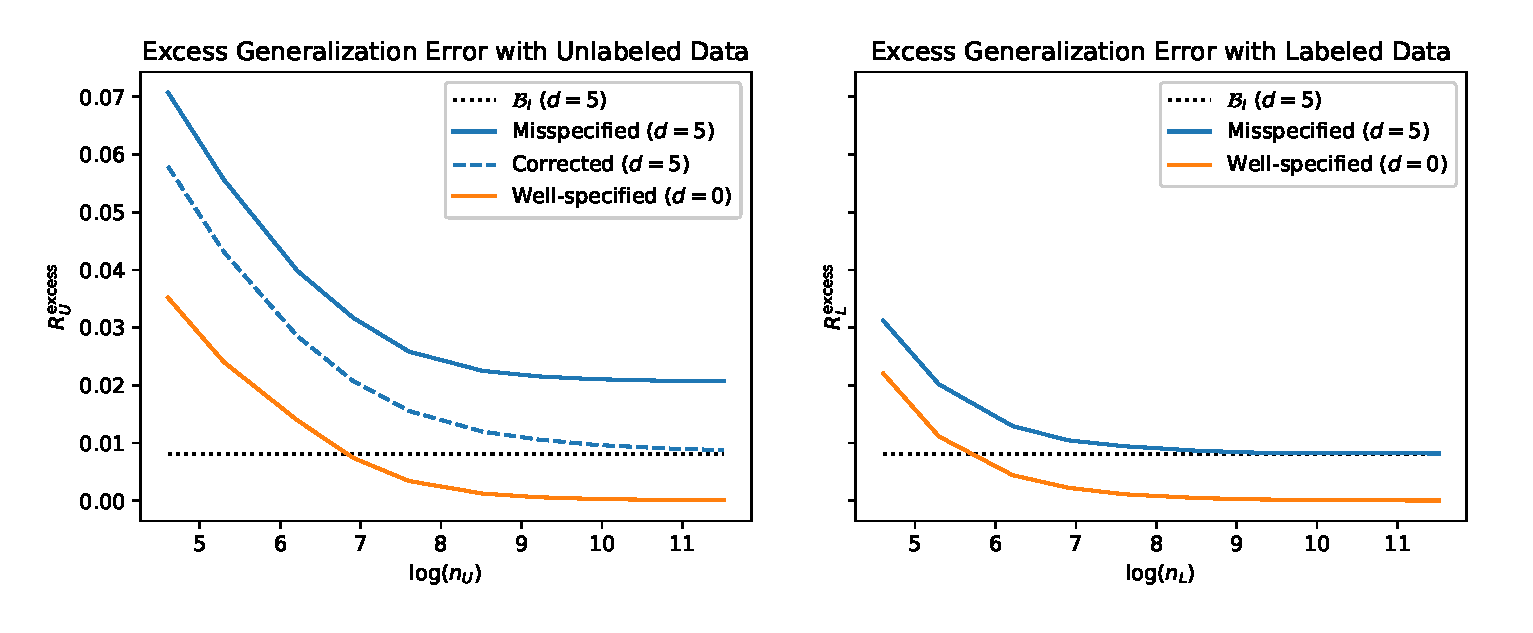
\includegraphics[width=.75\textwidth]{eps_figures/biases.eps}
    \else
    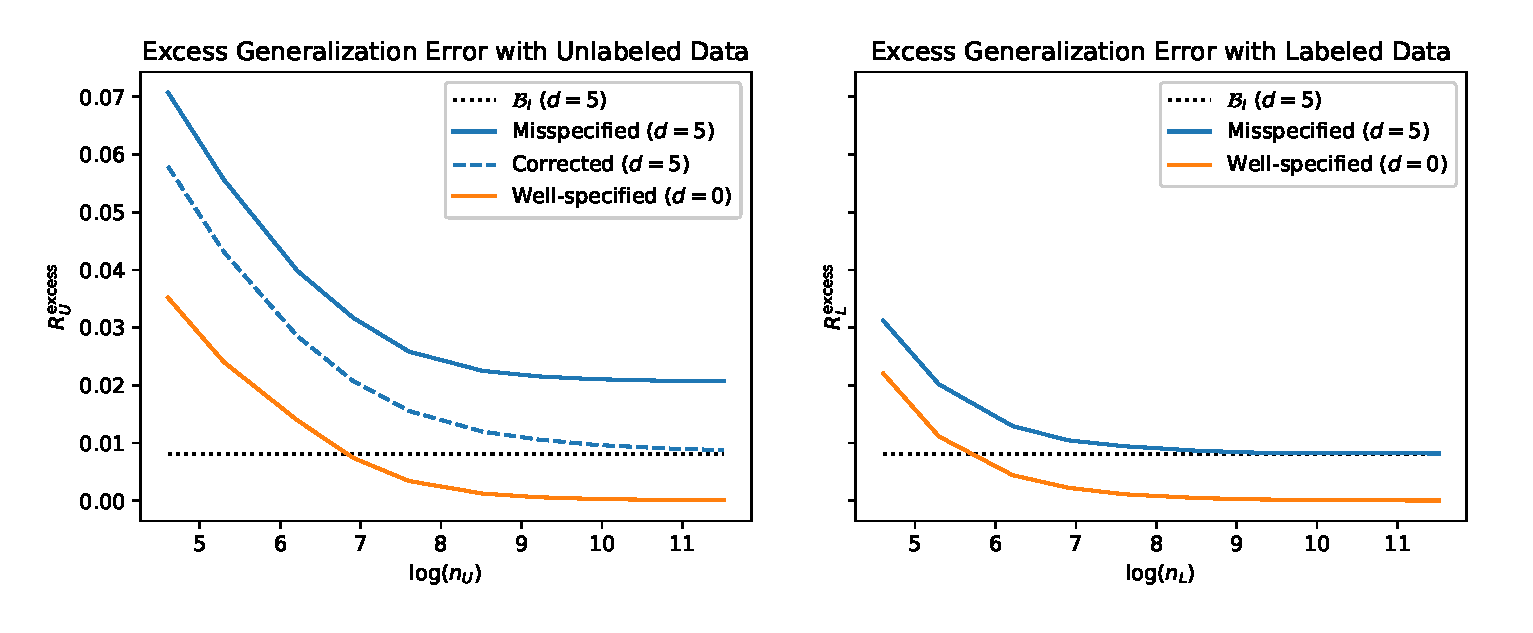
\includegraphics[width=.48\textwidth]{eps_figures/biases.eps}
    \fi
    %
    \caption{Excess generalization error vs. $\log(n)$ with different estimators for synthetic data. Left: comparison of unlabeled data performance under the three discussed settings. Right: comparison of labeled data performance for well-specified and misspecified models. A dashed line repesenting an empirical ``$\B_I$'' suggests how inference bias is present in both data cases. % With no misspecification ($d=0$) the labeled and unlabeled estimators both converge to an asymptotic error of zero. Under misspecification ($d=5$), we see that learning from unlabeled data results in an additional $\B_{\mathrm{est}}$ standing bias due to misspecification, and median aggregation corrects for this bias so that error converges to $\B_I$.
    }
    \label{fig:gen_err}
\end{figure}
\section{Applications}\label{sec:applications}
\vspace{-.5em}
Based on our generalization error framework, we now have a rigorous way to analyze misspecification in latent variable models. We examine two practical applications of our theoretical results in three settings---well-specified, misspecified, and corrected.
\begin{itemize}
    % \item \textbf{Correcting for misspecification:} for the weakly labeled data setting, we propose a simple algorithm improving over random selection of triplets $\lf_i, \lf_j, \lf_k$ that removes the error term $\varepsilon_{\max} \left(\frac{c_1 d}{m} + \frac{c_2}{\sqrt{n_U}} + \frac{c_3}{n_U}\right)$ given that $m$ is large and $d$ is $o(m^2)$.
    \item \textbf{Understanding the value of labeled data:} we address our motivating question about the value of labeled data–is a few labeled samples or many unlabeled samples better? This decision depends on the misspecification parameters ($d$, $\varepsilon_{\max}$), and $n_U$ versus $n_L$.
    \item \textbf{Combining labeled and unlabeled data:} we show how simple linear combinations of the estimators can improve generalization error bounds over using one or the other. Then, we suggest a James-Stein type estimator from~\cite{GreenStrawderman2001}, which combines an unbiased estimator with biased information, to easily determine the weights of the linear combination. %Based on our misspecification analysis, we show that this estimator offers a \textcolor{red}{X} improvement in generalization error. 
\end{itemize}

%In this section, we discuss these two consequences of our framework theoretically. In section \ref{sec:exp}, we verify them on synthetic and real data.


\subsection{Understanding the value of labeled data}
\vspace{-0.5em}
We use our analysis from section \ref{subsec:scaling} to develop a criterion for deciding between labeled and unlabeled points. Compute
\[\alpha(n_U) = \min_{n_L \in \mathbb{N}} \text{ s. t. } R_L^{e}(n_L) \le R_U^{e}(n_U),\]
%where $U^{\text{unlabeled}}, U^{\text{labeled}}$ are the upper bounds on the excess generalization error for unlabeled and labeled data, respectively.
and define
%\begin{align}
$V(n_U) = {n_U}/\alpha(n_U)$
%\end{align}
to be the \textit{data value ratio}. The intuitive idea here is to compare, for each amount of unlabeled data $n_U$, what factor less labeled data we would require to produce an equivalent error bound. We consider an approximation of the data value ratio $\widetilde{V}(n_U)$ based on our upper bounds for excess generalization error in \ref{subsec:scaling}. We examine the differences in $\widetilde{V}(n_U)$ for our three aforementioned settings:
\begin{itemize}
    \item Well-specified setting: comparing excess risk when $d = 0$ and $\varepsilon_{\max} = 0$ reduces to examining $\frac{m}{2n_L}$ and $\frac{c_4 m}{n_U}$. Thus $\widetilde{V}(n_U) = 2c_4$ and our framework suggests that labeled data is only a constant factor more beneficial than unlabeled data.
    \item Misspecified setting: $\widetilde{V}(n_U)$ will capture the tradeoff between $\frac{m}{2n_L}$ and $\B_{\mathrm{est}} + \frac{c_4 m }{n_U}$. We find that $\widetilde{V}(n_U) = 2 \varepsilon_{\max} \left(\frac{c_1 dn_U}{m} + \frac{c_2 \sqrt{n_U}}{m} + +\frac{c_3 d}{m^2} \right) + 2 c_4$. That is, the value of labeled data \textit{increases linearly in the amount of unlabeled data and misspecification} due to the standing bias in the generalization error for the unlabeled approach.  
    \item Corrected setting: under our conditions from Proposition \ref{prop:medians}, we examine the difference between $\frac{m}{2n_L}$ and $ c_\rho m \rho_{n_
    U}$, and thus $\widetilde{V}(n_U) = 2n_U c_{\rho} \rho_{n_U}$. Since $\rho_{n_U}$ converges to $0$, $\widetilde{V}(n_U)$ is sublinear in $n_U$, showing that the \textit{corrected model increases the relative value of unlabeled data.}
\end{itemize}

\vspace{-0.5em}
\paragraph{Synthetic Experiments} We measure $V(n)$ in well-specified, misspecified and corrected settings on synthetic data with the same setup as previously discussed. Our detailed protocol for approximating $V(n)$ is in the Appendix. 
%We expect three principles to hold: first, for a well-specified model, the data value ratio is small and roughly constant, second, the ratio scales with misspecification and finally, the ratio is smaller for a corrected model than for a misspecified model. \bcw{Get rid of this sentence?} We also expect that our theoretical ratio produces a reasonable estimate of the empirical value, in particular one that tracks the scaling of the misspecification level. 
We present the results in \autoref{fig:data_value_ratio}. In the well-specified case ($d = 0$), $V(n)$ is small (less than $5$) and roughly constant across $n$. Under misspecification however, the data value ratio grows with both $d$ and $n$ albeit much more slowly for the corrected setting, aligning with our theoretical findings.

\begin{figure}
    \centering
    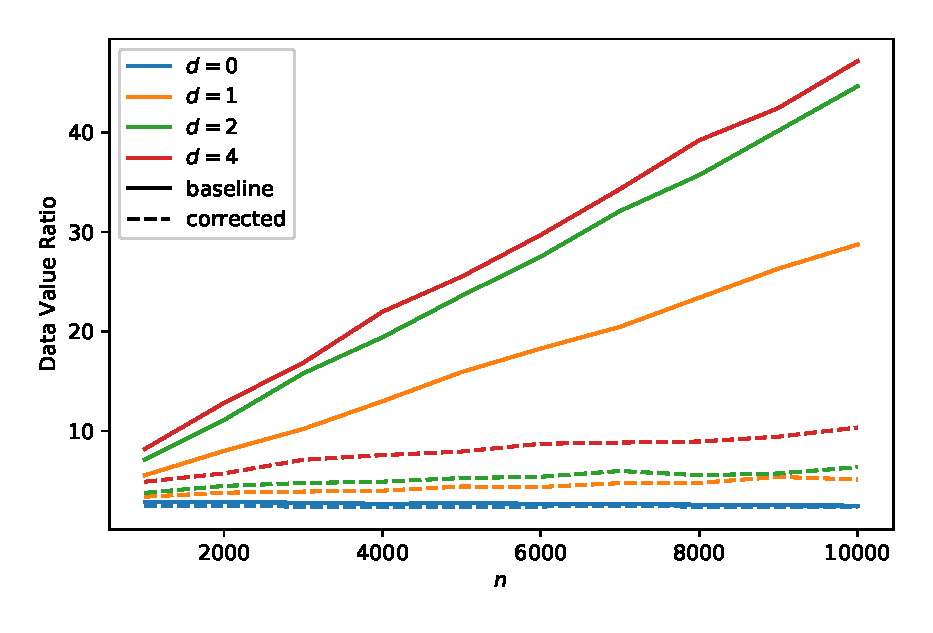
\includegraphics[width=.3\textwidth]{eps_figures/data_value_ratio_vs_n.eps}
    %
    \caption{Data value ratio vs. $n$, using both the standard method-of-moments approach and the corrected approach, which aggregates results over triplets using medians. Note that $d=0$ represents the well-specified setting. %We see that in the well-specified case ($d=0$) the data value ratio is small and roughly constant across $n$. Under misspecification, the data value ratio grows with $d$ for both the baseline and corrected models, but grows faster for baseline models, as reflected by our theoretical model.
    }
    \label{fig:data_value_ratio}
\end{figure}

%Based on Theorems \ref{thm:labeled} and \ref{thm:unlabeled}, we see that this ratio captures the tradeoff between $\varepsilon_{\max} \big(\frac{c_1 d}{m} + \frac{c_2 m}{\sqrt{n_U}} + \frac{c_3 m}{n_U} \big) + \frac{c_4 m}{n_U}$ and $\frac{m}{2n_L}$. In particular, %for a weakly labeled dataset to have a better generalization error, 
% we must have that $\alpha(n) = c\big(\frac{\varepsilon_{\max} n m^2}{m^2 - \varepsilon_{\max} d n}\big)^2$ for some constant $c$ and $n < \frac{m^2}{\varepsilon_{\max} d}$; when $n$ is too large, it is possible that no amount of unlabeled data can achieve the same generalization error due to the standing bias. Therefore, as any  one of $n, \varepsilon_{\max}$, or $d$ increases, the threshold for weakly labeled points becomes higher. On the other hand, if we were to ignore misspecification, we only require that $V(n) = 2c_4$ be a constant value, which as a criterion could lead to wrong decisions if the model is actually incorrect.
% We use our analysis from section \ref{subsec:scaling} to develop a criterion for deciding between $n_L$ labeled points and $n_U$ weakly labeled points. Let $n = n_L$, and then compute
% \[\alpha(n) = \min_{n_U \in \mathbb{N}} \text{ s. t. } U^{\text{unlabeled}}(n_U) \leq U^{\text{labeled}}(n),\]
% where $U^{\text{unlabeled}}, U^{\text{labeled}}$ are the upper bounds on the excess generalization error for unlabeled and labeled data, respectively.
%
% Then, the ratio
% %\begin{align}
% $V(n) = \alpha(n)/{n}$
% %\end{align}
% represents the value of labeled over weakly labeled data. The intuitive idea here is to compare, for each amount of labeled data $n$, what factor greater unlabeled data we would require to produce an equivalent error bound. 
% Based on Theorems \ref{thm:labeled} and \ref{thm:unlabeled}, we see that this ratio captures the tradeoff between $\varepsilon_{\max} \big(\frac{c_1 d}{m} + \frac{c_2 m}{\sqrt{n_U}} + \frac{c_3 m}{n_U} \big) + \frac{c_4 m}{n_U}$ and $\frac{m}{2n_L}$. In particular, %for a weakly labeled dataset to have a better generalization error, 
% we must have that $\alpha(n) = c\big(\frac{\varepsilon_{\max} n m^2}{m^2 - \varepsilon_{\max} d n}\big)^2$ for some constant $c$ and $n < \frac{m^2}{\varepsilon_{\max} d}$; when $n$ is too large, it is possible that no amount of unlabeled data can achieve the same generalization error due to the standing bias. Therefore, as any  one of $n, \varepsilon_{\max}$, or $d$ increases, the threshold for weakly labeled points becomes higher. On the other hand, if we were to ignore misspecification, we only require that $V(n) = 2c_4$ be a constant value, which as a criterion could lead to wrong decisions if the model is actually incorrect.

%Equivalently, we require that $d$ must be of order  $o\big(\frac{m^2}{\varepsilon_{\max}}\big(\frac{1}{n_L} - \frac{1}{\sqrt{n_U}}\big)\big)$ for a weakly labeled dataset to have better generalization error. 


%Therefore, when $d$ and $\varepsilon_{\max}$ are both small while $n_L$ is also small, $V(n)$ should suggest a reasonably-sized $n_U$ in order for an unlabeled dataset to yield higher performance. On the other hand, when there are many unmodeled dependencies and all of them are strong, $V(n)$ should be very large, suggesting that a small labeled dataset performs better.

\subsection{Combining labeled and unlabeled data}
\vspace{-0.5em}
While we now have a criterion to choose between datasets, how do we combine information from both? We examine ways to combine the accuracy parameters, namely $\widetilde{a}^U$ as defined in \eqref{eq:triplet} for unlabeled data and an equivalent $\widetilde{a}^L := \Ehat{\bm{\lf} Y}$ for labeled data. Recall that $\widetilde{a}^L$ is unbiased, while $\widetilde{a}^U$ is both biased and inconsistent. 

First, we consider a simple linear combination, $a^{\mathrm{lin}}(\alpha) = \alpha \widetilde{a}^U + (1 - \alpha) \widetilde{a}^L$ for some $\alpha \in [0, 1]$. Using our framework in \ref{thm:decomposition}, we can derive similar upper bounds on excess generalization error when the estimator is $a^{\mathrm{lin}}(\alpha)$. We summarize our findings across the three settings below, where for the corrected setting we consider $\alpha \widetilde{a}^M + (1 - \alpha) \widetilde{a}^L$. 
\begin{itemize}
    \item Well-specified setting: the upper bound on excess generalization error using $a^{\mathrm{lin}}$, ignoring $\B_I$ and lower order terms, is $\alpha^2 \frac{c_4 m}{n_U} + (1 - \alpha)^2 \frac{m}{2n_L}$. One can easily verify that there exists an $\alpha \in (0, 1)$ that minimizes this upper bound. Since $n_U$ is usually much larger than $n_L$, plugging in this optimal $\alpha$ shows that this new upper bound is roughly of the same order as the unlabeled case.
    \item Misspecified setting: the upper bound is a cubic polynomial in $\alpha$. We find that the standing bias results in a generally lower optimal $\alpha$ and suggests that a combined estimator can yield an upper bound much smaller than that for the unlabeled case. 
    \item Corrected setting: the upper bound now consists of $\alpha^2 c_{\rho} m \rho_{n_U} + (1 - \alpha)^2 \frac{m}{2n_L}$. As a function of $\alpha$, this differs from the well-specified setting's expression only in constant coefficients, so this again suggests an optimal $\alpha \in (0, 1)$ and performance roughly similar to the unlabeled case.
\end{itemize}

% We produce an upper bound on excess generalization error from using $a^{\mathrm{lin}}$ similar to our results in Theorems \ref{thm:labeled} and \ref{thm:unlabeled}.
%\begin{align}
%    R_{\mathrm{lin}}^{\mathrm{excess}}(\alpha)\le & \varepsilon_{\max}\Big(\frac{c'_1 \alpha d }{m} + \frac{c'_2 \alpha^2 }{\sqrt{n_U}} + \frac{c'_3 \alpha^3 d}{m n_U} \\
%    &+ \frac{\alpha (1 - \alpha)^2 c'_5 d}{m n_L} \Big) + \frac{c'_4 \alpha^2 m}{n_U} \nonumber \\
%    &+ \frac{(1 - \alpha)^2 m}{2n_L} + \B_I + o(1/n_L), \nonumber
%\end{align}
% \mayee{need to change into structure that parallels 5.1. Basically we say that for misspecified case, gen err is cubic polynomial in $\alpha$ and suggests that no local minimum in $(0, 1)$ unless $n_L$ is small (i.e. we usually just want to use labeled data, unlabeled is not good). For well-specified and corrected case, gen err is $\alpha^2 \Var{U}{n_U} + (1 - \alpha)^2 \Var{L}{n_L}$, and this yields an $\alpha \in (0, 1)$ given our variance constants are different enough, i.e. labeled data value is ``reduced''}.

%where $c'$ are scaled from the constants used in Theorems \ref{thm:labeled} and \ref{thm:unlabeled}. It is possible that this upper bound is minimized using some $\alpha \in (0, 1)$, especially when $n_L$ is small, which would suggest that a simple linear combination of the two estimators does better than using either one of them. We test a range of $\alpha$ on our synthetic datasets to confirm this.

%From Lemma \ref{lemma:accuracy_bias}, we see that $\widetilde{a}_i^U$ is biased while $\widetilde{a}_i^L$ is not. At first glance, it would seem that we should simply rely on the unbiased estimator---however, as known from Stein's phenomenon, this is not necessarily the right approach.
In practice, we do not know the exact $\alpha$ that optimizes generalization error. However, there is vast literature on combined estimators that dominate the MLE estimator $\widetilde{a}^L$. In particular, we suggest using an approach from~\cite{GreenStrawderman2001}, who propose a way of setting $\alpha$ given knowledge of an unbiased estimator with biased information. % the following combined estimator:
%\begin{align}
%    \bar{a} := \widetilde{a}^U + \bigg(1 - \frac{r}{(\widetilde{a}^L - \widetilde{a}^U)^T \Sigma^{-1} (\widetilde{a}^L - \widetilde{a}^U)} \bigg)_{\mathclap{+}} (\widetilde{a}^L - \widetilde{a}^U),
%\end{align}
%\begin{align}
%    \bar{a}_i := \widetilde{a}_i^L - \frac{(m - 2) }{n_L \|\widetilde{a}_i^L - \widetilde{a}_i^U \|_2^2} (\widetilde{a}_i^L - \widetilde{a}_i^U)
%\end{align}
%where $\Sigma = \Cov(\widetilde{a}^L)$, and $r \in [0, 2(m - 2)]$.  
%They show that this estimator dominates $\widetilde{a}^L$ when the unbiased estimator is Gaussian and its covariance is known. However, since we can only estimate the covariance matrix, we replace $\Sigma$ with an empirical estimate $\hat{\Sigma}$. Moreover, since $\widetilde{a}^L$ is only Gaussian asymptotically, we do not provide theoretical guarantees on $\bar{a}$ but instead empirically validate its performance. \todo{story here: this estimator builds upon naive linear combination (just how to set the $\alpha$) }

%This estimator has been proven to dominate the unbiased $\widetilde{a}^L$ when the true covariance matrix $\Sigma$ is known, even when $\widetilde{a}^U$ is very biased \steve{we don't have normality though, right?}. %In particular, \cite{GreenStrawderman1991} show that
%Using their equation 2.5, it is true that
%\begin{align}
%    &\E{}{\|\bar{a} - a \|_2^2} \le m Var(\widetilde{a}_i^L) - \nonumber \\
%    &\frac{Var(\widetilde{a}_i^L)^2 (m - 2)^2}{\|\E{}{\widetilde{a}^U} - a \|_2^2 + (m - 2)(\sqrt{Var(\widetilde{a}_i^L)} + Var(\widetilde{a}_i^U))} \nonumber
%\end{align}

%which, when plugged into our decomposition framework in Theorem \ref{thm:decomposition}, gives us a better generalization error \todo{be more precise here.}

%We now show that the label model generalization error using $\bar{a}$ is better than that using either $\widetilde{a}_i^U$ or $\widetilde{a}_i^L$. \todo{plug above eqn into thm 1 type bound}.

\vspace{-0.5em}
\paragraph{Synthetic Experiments} We investigate the empirical performance of estimators which combine labeled and unlabeled data in well-specified, misspecified and corrected settings. We measure both the error when using the optimal $\alpha$ and the more practical approach of \cite{GreenStrawderman2001}. We fix $n_U=1000$ and vary $n_L$ across a range of smaller values, aligning with the assumption that many more unlabeled than labeled points are typically available. Our results are in Figure \ref{fig:combined}. In the well-specified setting, the combined estimators perform roughly the same as just $\widetilde{a}^U$, matching up with our theoretical observations for large $n_U$. In the misspecified setting, both combined estimators result in much lower excess risk than either estimator individually, and as $n_L$ increases, the labeled estimator curve approaches those of the combined estimators, suggesting that the weight on $\widetilde{a}^L$ increases as more labeled data becomes available. Lastly, in the corrected setting both combined estimators perform better than $\widetilde{a}^U$, but not by much.
%suggesting that there is a standing bias present in the former case that makes combining with labeled data more helpful.
%The approach of \cite{GreenStrawderman2001} does not consistently outperform the unlabeled only approach in the well-specified case, where the unlabeled estimator is unbiased. However, it significantly outperforms either individual approach in the misspecified case and outperforms either individual approach in the corrected case. 
The weights $\alpha$ are reported in the Appendix. The optimal weights for the well-specified and corrected settings are higher (i.e. more weight on the unlabeled estimator) than the misspecified setting, and these weights decrease with $n_L$.

%We expect that in the well-specified case, the combined estimators won't significantly outperform the unlabeled estimator. On the other hand, under misspecification, we expect the combined estimators, which account for the standing bias of unlabeled data, to provide a superior estimate to either individual estimator. Finally, for the corrected case, we expect more modest improvements from combining labeled and unlabeled data, similarly to the well-specified case. As the estimator proposed by \cite{GreenStrawderman1991} assumes that the unlabeled estimator is biased, we expect it to perform the best in the misspecified case compared to the optimal combined estimator. We present the results in \autoref{fig:combined}.

% We further expect the James-Stein-type estimator to perform better under misspecification where the unlabeled estimator is biased and the simple linear combination to perform better for well-specified models. Results in \autoref{fig:combined}.

\begin{figure}
    \centering
    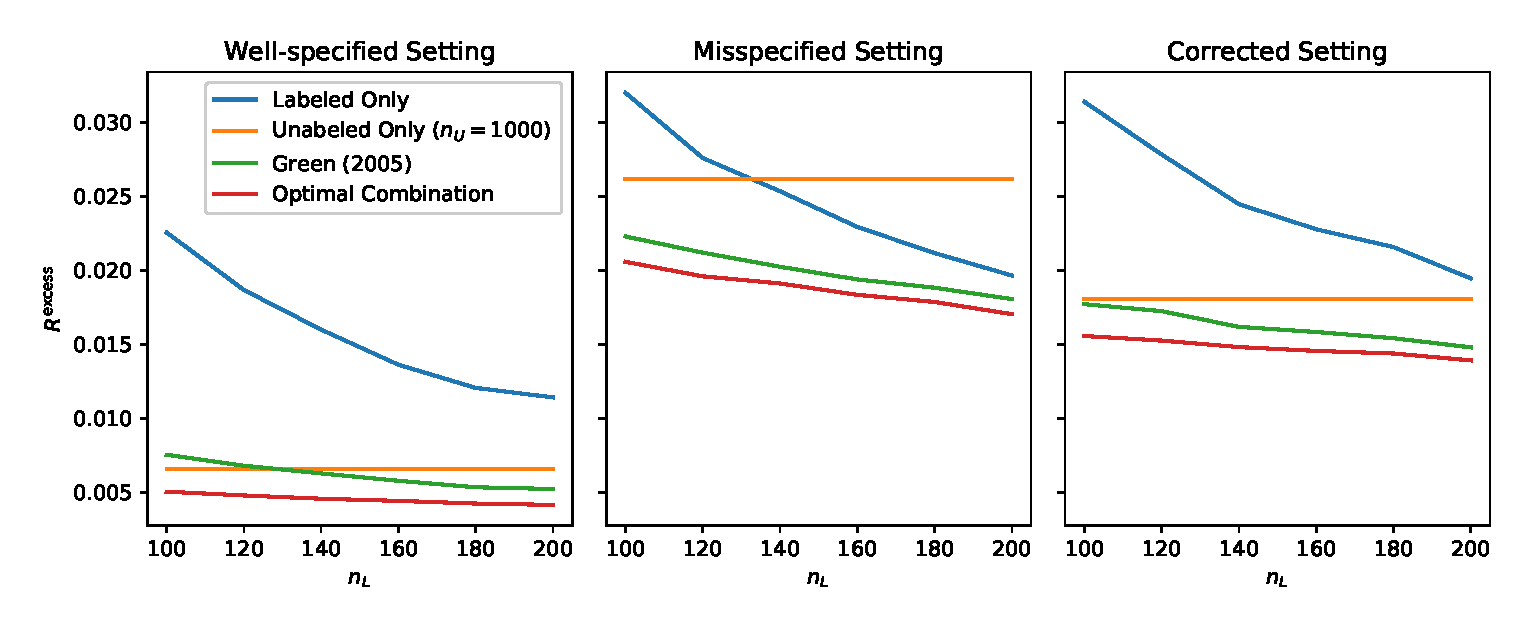
\includegraphics[width=.48\textwidth]{eps_figures/combined.eps}
    %
    \caption{Excess generalization error for an optimally weighted combination of labeled and unlabeled estimators, and a combination weighted according to \cite{GreenStrawderman2001} across the well-specified (left), misspecified (center), and corrected (right) settings. The number of unlabeled points is fixed at $n_U=1000$. %The approach of \cite{GreenStrawderman2001} does not consistently outperform the unlabeled only approach in the well-specified case, where the unlabeled estimator is unbiased. However, it significantly outperforms either individual approach in the misspecified case and outperforms either individual approach in the corrected case. The combination weights are reported in the \todo{Appendix}. Broadly, the optimal weights for the well-specified and corrected settings are higher than the misspecified setting, and these weights decrease with $n_L$.
    }
    \label{fig:combined}
\end{figure}
\section{Experiments} \label{sec:exp}
% We evaluate our theoretical findings and our proposed criterion. We anticipate that the value of data is significantly affected by misspecification, so that labeled data offers an insignificant value versus unlabeled (i.e., a small value ratio) for a well-specified model, but becomes more valuable as the misspecification level increases. We hypothesize that combining both labeled and unlabeled data can offer a superior estimate (as compared to relying one or the other alone). Finally, we expect that the bias due to misspecification is reflected downstream for a variety of models. 

% \subsection{Synthetic Data}

% \paragraph{Protocol}

% Our synthetic data distributions have balanced classes (i.e., $\mathbb{E}[Y]=0$) and $m=10$ labeling functions, with accuracies drawn uniformly from $[0.55, 0.75]$. Dependency strengths are fixed at $\varepsilon_{ij}=0.1$. To measure the expected generalization error of each learning algorithm for a given budget $n$, we perform $1000$ trials and average results, drawing data independently for each trial.

% {\color{red} Combination table goes here. Shows four columns: all labeled, all unlabeled, naive combination, and James-Stein.}


We validate our findings on a real-world dataset. We expect that some amount of misspecification is inevitable, and that this misspecification causes additional bias when learning from only unlabeled data. Unlike our theoretical setting where we limit the number of dependencies $d$ for simplicity, with real-world data we anticipate many small dependencies which cannot be completely corrected by the medians approach. We seek to answer the following key questions in this real-world setting.

\begin{itemize}
    \item What is the standing parameter estimation bias due to misspecification? 
    
    \item To what extent does the corrected estimator mitigate this bias?
    
    \item What is the data value ratio for the corrected estimator? \steve{I like the other questions; maybe this question isn't necessary though? The standing bias means the labeled data ratio will depend on $n_U$} \bcw{I think I agree with the fact that the plot won't be very informative (it'll just be a line) but might be nice to have just to parallel the theoretical results.}
    
    \item Can a combined estimator with access to a small amount of labeled data provide substantial benefits over using only unlabeled data?
\end{itemize}

\paragraph{Protocol} Our real-world task is the sentiment analysis task of determining whether IMDB movie reviews are positive or negative \citep{maas2011learning}. The dataset contains 50K movie reviews, which we split into a training set of 35K reviews and validation and test sets of 7.5K reviews each. For our weak supervision sources, we use the following simple heuristics: For each word  of ``love'', ``like'', ``good'', ``great'', ``best'', ``excellent'' we write a labeling function which votes positive when the word appears, and negative otherwise. For each word of ``terrible'', ``worst'', ``bad'', ``better'', ``could'', ``would'' we similarly write a labeling function which votes negative when the word appears, and positive otherwise. We use these words because they are empirically predictive and intuitively associated with positive/negative reviews.

% \steve{how did you pick the words? Especially the negative ones seem a little counterintuitive.} \bcw{I sorted words according to predictive power, and picked ones which seemed intuitive. I'm guessing you're referring to ``better'', ``could'' and ``would'' when you talk about the counterintuitive ones. These actually make sense to me, as they're referring to things like ``could have been better''} \steve{Can you add a few words describing the process then? Maybe: ``we chose words that were predictive and intuitive'' or something like that}

\todo{Talk about singleton potentials}. As a proxy for generalization error in our experiments, we use the cross entropy loss on a test set.
% We measure model performance in terms of its F1-score on the test set as a proxy for generalization error.
% For each dataset we train models with different label budgets $n_L$. We report the average accuracy on the test set over $1000$ trials (with different points to label selected for each trial). 

\paragraph{Standing bias and correction}

For our first real-world experiment, we measure the standing parameter estimation bias when learning from unlabeled data $\mathcal{B}_\text{est}$, and measure the decrease in this bias when using a corrected estimator. Recall that a corrected estimator has an asymptotic parameter estimation bias of zero when $d<\frac{(m-1)(m-2)}{4}$ for reasonable values of $m$ and $n$. In this real-world setting, we anticipate many small dependencies; $d$ might even be $m \choose 2$ but with most $\varepsilon_{ij}$ quite small. Hence, we anticipate that the corrected estimator reduces $\mathcal{B}_\text{est}$ by mitigating the effects of larger dependencies while still being biased by the many small dependencies. We compute the test cross entropy loss for a labeled model, a baseline unlabeled and an unlabeled model with correction while varying $n$ and report results in \autoref{fig:real_biases}. Losses appear to converge, with a large gap between the labeled and unlabeled models and a smaller gap between the labeled model and the unlabeled model with correction.

\begin{figure}
    \centering
    \begin{subfigure}{.25\textwidth}
      \centering
      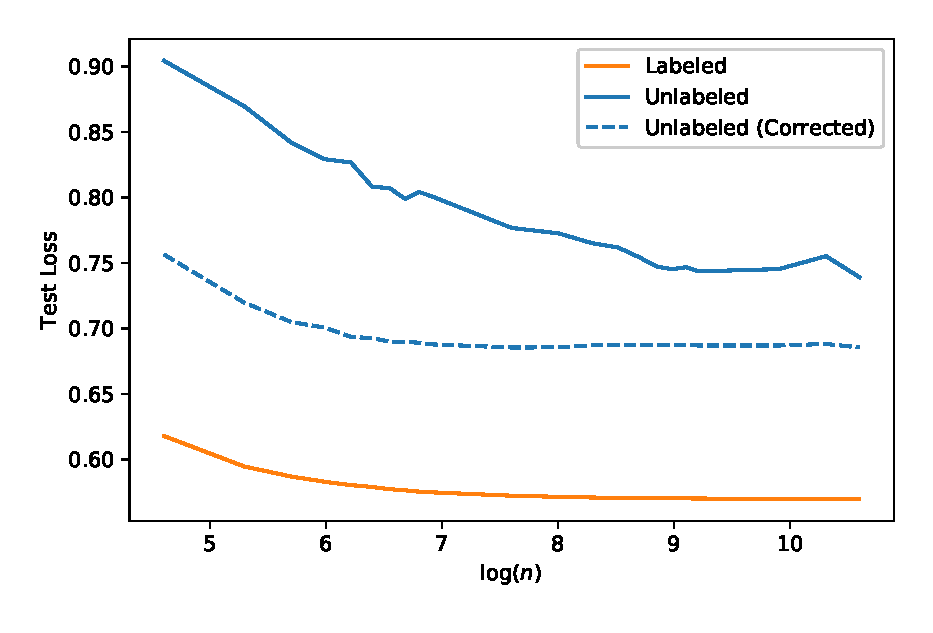
\includegraphics[width=\linewidth]{eps_figures/real_biases.eps}
     % \caption{A subfigure}
     % \label{fig:sub1}
    \end{subfigure}
   %
    \begin{subfigure}{.4\textwidth}
      \centering
      \begin{small}
      \begin{tabular}{lccr}
      \hline
      \vskip -0.1in
      Model & $\text{Loss}_\text{40K}$ & $\text{F1}_\text{40K}$ \\
      \hline
      Labeled & .570 & 71.79 \\
      Unlabeled & .740 & 64.81 \\
      Corrected & .686 & 68.12 \\
      \hline
      \end{tabular}
      \end{small}
     % \caption{A subfigure}
     % \label{fig:sub1}
    \end{subfigure}
    \caption{}
    \label{fig:real_biases}
\end{figure}

\paragraph{Measuring the value of labeled data} Next, we measure the data value ratio in the real-world setting. Since both the unlabeled model and the unlabeled model with correction have a standing bias compared to the labeled model, we anticipate that the data value ratio for both unlabeled approaches grows with $n$, with the data value ratio for the baseline unlabeled model growing faster due to its higher bias. We report these results in \autoref{fig:real_data_value_ratio}.

\begin{figure}
    \centering
    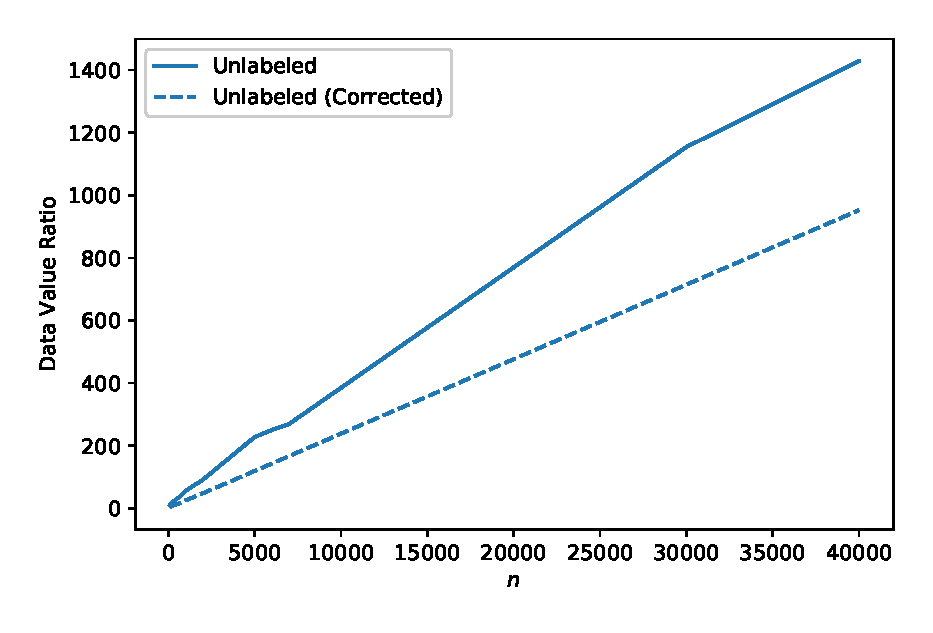
\includegraphics[width=.4\textwidth]{eps_figures/real_data_value_ratio.eps}
   %
    \caption{}
    \label{fig:real_data_value_ratio}
\end{figure}

\paragraph{Combining labeled and unlabeled data} We finally measure the performance of the combined estimator from \cite{GreenStrawderman2001} in the setting where a small number of labeled points and many unlabeled points are available. We let $n_U=40,000$ be the entire training set and vary $n_L$ between $40$ and $400$. We use the more performant corrected estimator for learning from unlabeled data. We report the F1 score, which is typically used to measure the performance of weak supervision methods. Results are in \autoref{tab:real_combo}. We observe that the combined estimator outperforms either approach individually for $n_L>40$.

% We use three tasks. First, \textbf{Spam} classification for Youtube comments ~\citep{alberto2015tubespam} has $10$ LFs from~\cite{Ratner19}. Here, the training set has $1586$ examples and the test set has $250$ examples; classes are approximately balanced. 

% In this case, we do not a priori know the level of misspecification. We expect that LFs are neither completely conditionally independent nor so markedly (conditionally) dependent that nothing can be learned from unlabeled data. This leads to data value ratios that are in between the scenarios in between the two extreme synthetic cases we considered above.

\begin{table}[t]
\caption{F1-scores for unlabeled, labeled and combined approaches on the IMDB dataset. }
\label{tab:real_combo}
\vskip 0.15in
\renewcommand{\arraystretch}{1.25} % Default value: 1
\begin{center}
\begin{small}
\begin{tabular}{lccccr}
\hline
$n_U$ & $n_L$ & $\text{F1}_\text{Unlabeled}$ & $\text{F1}_\text{Labeled}$ &  $\text{F1}_\text{Combined}$ \\
\hline
40,000 & 40 & 68.12 & 64.70 & 67.06 \\
40,000 & 80 & 68.12 & 67.65 & 68.81 \\
40,000 & 120 & 68.12 & 68.92 & 69.64 \\
40,000 & 200 & 68.12 & 69.97 & 70.41 \\
40,000 & 400 & 68.12 & 70.81 & 71.04 \\
\hline
\end{tabular}
\end{small}
\end{center}
\vskip -0.1in
\end{table}

% \begin{table}[t]
% \caption{F1-scores for weakly labeled, labeled and hybrid approaches over the \textbf{Spam} and \textbf{Spouse} datasets.}
% \label{sample-table}
% \vskip 0.15in
% \renewcommand{\arraystretch}{1.25} % Default value: 1
% \begin{center}
% \begin{small}
% \begin{tabular}{lcccccr}
% \hline
% \textbf{Task} & $n_U$ & $n_L$ & \bfseries{\scshape{FS}} & \bfseries{\scshape{MLE}} & \bfseries{\scshape{Comb.}} \\
% \hline
% Spam    & 1586 & 40 & 82.35 & 82.40 & 83.16 \\
% Spouse  & 3858 & 50 & 19.30 & 19.23 & 22.93 \\
% \hline
% \end{tabular}
% \end{small}
% \end{center}
% \vskip -0.1in
% \end{table}

% \begin{figure}
%     \centering
%     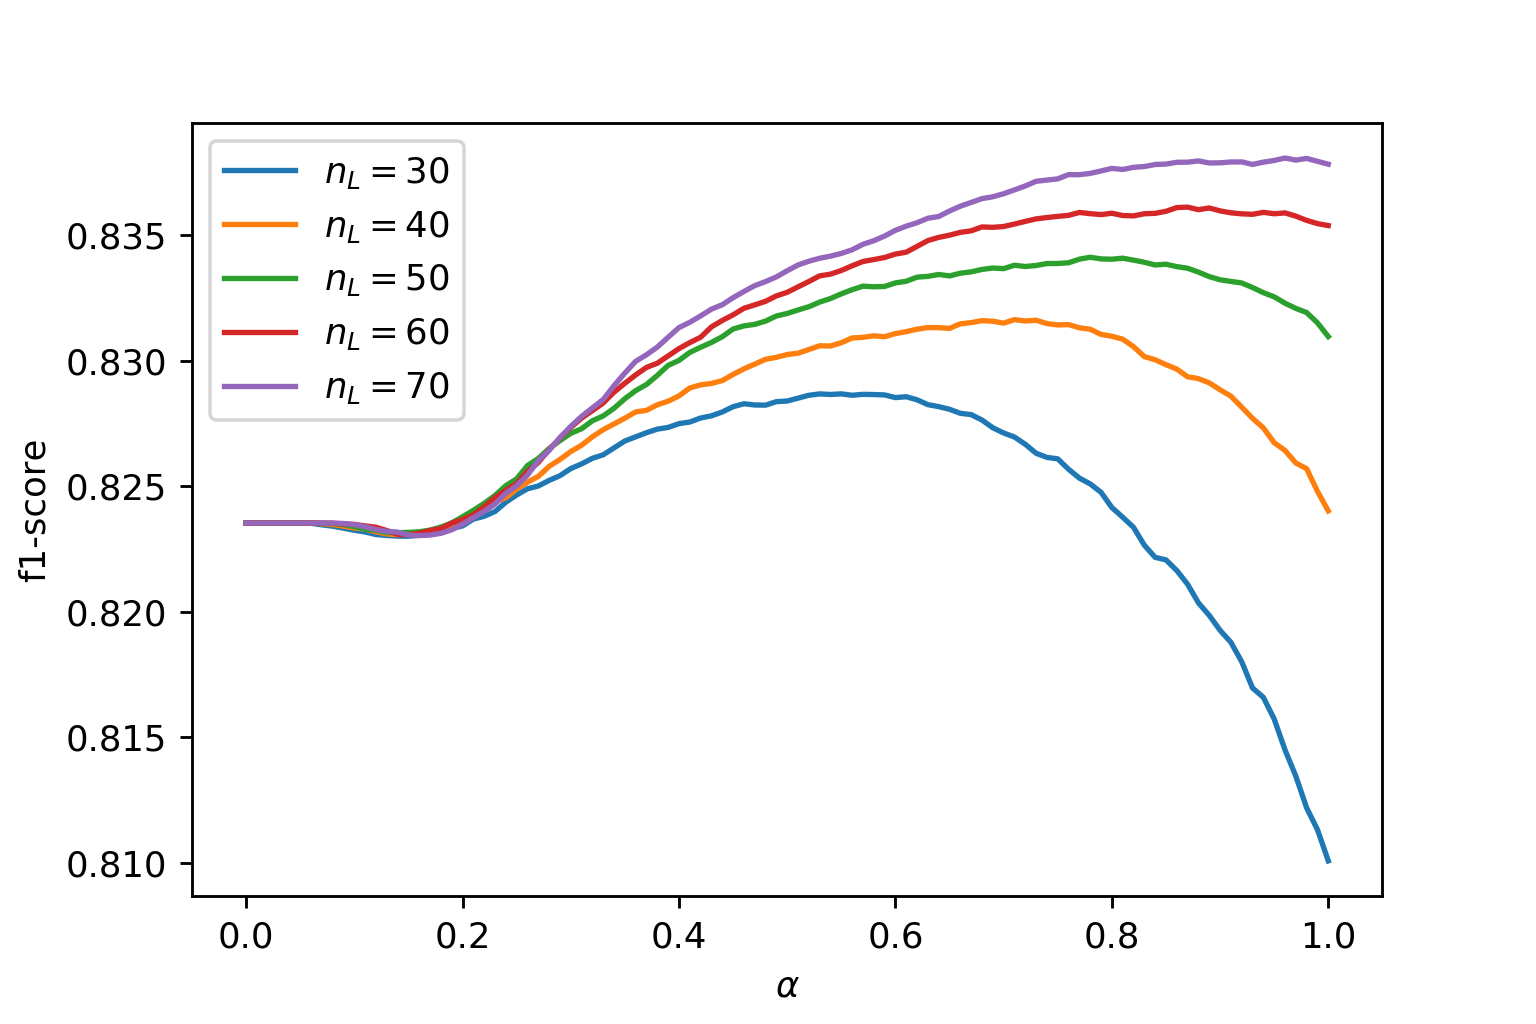
\includegraphics[width=.48\textwidth]{figures/spam_combined_estimator.png}
%     \caption{F1-score of a combined estimator varying combination weight $\alpha$ on the \textbf{Spam} dataset for different labeled budgets $n_L$ (the weakly labeled budget is the entire dataset). We see that combining labeled and weakly labeled approaches can outperform either individually.}
%     \label{fig:spam_combined_estimator}
% \end{figure}

% \subsection{Weak Labels, Standing Bias, and Downstream Models}
% Next, we measure the impact of bias in weak labels on end models trained on weak labels. We expect that when the weak labels do not have a standing bias, the generalization error is asymptotically identical to the case of training on fully-supervised labels. On the other hand, we hypothesize that biased weak labels will be reflected with a biased downstream model, no matter how much data we use, and that this bias is also a function of misspecification. That is, we expect that downstream models may not always be robust to weak labels.
% 
% \paragraph{Protocol}
% {\color{red} Gathering models for this step.}
% 
% \paragraph{Results}
% {\color{red} todo}

% \begin{figure}
%     \centering
%     \begin{minipage}{0.49\textwidth}
%         \centering
%         \includegraphics[width=0.9\textwidth]{figures/spam.pdf}
%         \caption{Accuracy for the \textbf{Spam} dataset with different budgets of labels and different unlabeled data weights $\gamma$.}
%         \label{fig:spam}
%     \end{minipage}\hfill
%     \begin{minipage}{0.49\textwidth}
%         \centering
%         \includegraphics[width=0.9\textwidth]{figures/amazon_reviews_1000.pdf}
%         \caption{Accuracy for the \textbf{Amazon Reviews} dataset with different budgets of labels and different unlabeled weights $\gamma$.}
%         \label{fig:amazon_reviews}
%     \end{minipage}
% \end{figure}

% \section{Discussion and Related Work}

% In this exploration, we find that a small number of gold labels can be valuable within the data programming pipeline, suggesting that expert time might be best spent on a combination of providing high-level intuitions through labeling functions and individual gold labels. Alternate approaches for using a small number of gold labels remain to be studied. For example, instead of learning accuracies from gold labels, these labels could be used for semi-supervised training along with the noisy labels produced by the standard data programming process. 

% Co-training, proposed by \cite{blum1998combining}, 

% \cite{nashaat2018hybridization} propose hybridizing data programming with active learning by selecting data points to label where labeling functions disagree most, and ``correcting'' labeling functions on these examples. Our work differs from this approach in that we study how gold labels for a small numbers of randomly selected examples can be valuable, whereas they propose budgets in the thousands which can be actively selected.

% One limitation of our work is that the unlabeled weight parameter $\gamma$ must be tuned using validation data, as its optimal value depends on the number of data points available and the data distribution. Our experiments seem to indicate that smaller values of $\gamma$ perform better when the dependencies between labeling functions are more pronounced. For example, when conditional independence assumptions are met we find empirically that $\gamma=1$ is optimal but when dependencies exist (including on real datasets) the optimal value of $\gamma$ is much smaller. We leave it to future work to determine a more effective policy for selecting $\gamma$ that does not require additional validation data.




%\subsubsection*{Author Contributions}
%If you'd like to, you may include  a section for author contributions as is done
%in many journals. This is optional and at the discretion of the authors.

%\subsubsection*{Acknowledgments}
%Use unnumbered third level headings for the acknowledgments. All
%acknowledgments, including those to funding agencies, go at the end of the paper.


\bibliography{bibliography}

\clearpage
\appendix

\onecolumn

\aistatstitle{Supplementary Materials}
\section{Glossary}
\label{sec:gloss}


The glossary is given in Table~\ref{table:glossary} below.
\begin{table*}[h]
\centering
\small
\begin{tabular}{l l}
\toprule
Symbol & Used for \\
\midrule
$X$ & An input vector $X\in\mathcal{X}$.\\
$Y$ & A latent ground-truth label $Y\in\mathcal{Y}=\{-1,1\}$.\\
$m$ & Number of sources.\\
$\lf_j$ & $j$th source output $\lf_j: \mathcal{X} \rightarrow \mathcal{Y}$; all $m$ labels make up vector $\bm{\lf}$ \\
%$\bm{\lambda}$ & A vector of source outputs $\bm{\lambda}\in\mathcal{Y}^m$.\\
$\widetilde{Y}$ & Probabilistic label in $[-1, 1]$ output by the latent variable model.\\
$n_U$ & Number of unlabeled samples.\\
$n_L$ & Number of labeled samples.\\
$\Theta$ & Canonical parameters of the Ising model for $\Pr(Y,\bm{\lambda})$.\\
$G$ & Dependency graph $G=(V,E)$ over sources and the latent ground-truth label.\\
$E_\lambda$ & Edges among sources in $G$.\\
$d$ & Number of dependencies among sources $d=|E_\lambda|$.\\
$a_i$ & True accuracy of the $i$th source $\mathbb{E}[\lambda_iY]$.\\
$\widetilde{a}_i^U$ & Estimated accuracy of the $i$th source using unlabeled data via the triplet method.\\
$\widetilde{a}_i^L$ & Estimated accuracy of the $i$th source using labeled data, i.e. $\Ehat{\lf_i Y}$.\\
$\widetilde{a}_i^M$ & Estimated accuracy of the $i$th source using unlabeled data via the\\
& triplet method and median aggregation.\\
$\mathcal{N}$ & Random variable representing dataset used.\\
$\tau$ & Algorithmic randomness for estimating accuracies via triplet method.\\
$R,R_U,R_L,R_M$ & Generalization error $R = \mathbb{E}_{(Y, \bm{\lf}), \N, \tau}[l(\widetilde{Y}, Y)]$. $R_U,R_L,R_M$ are for $\widetilde{a}_i^U,\widetilde{a}_i^L,\widetilde{a}_i^M$, respectively, \\
& and $l(\cdot, \cdot)$ is the cross-entropy loss.\\
% $R_U$ & Generalization error when using the triplet method.\\
% $R_L$ & Generalization error when estimating accuracies empirically.\\
% $R_M$ & Generalization error when using the triplet method with median aggregation.\\
$R^e,R^e_U,R^e_L,R^e_M$ & Excess generalization error $R^e=R-H(Y|\bm{\lambda})$.\\
$\mathcal{B}_I$ & Inference bias $\mathcal{B}_I=\sum_{(i, j) \in E_\lf}I(\lf_i; \lf_j | Y)$.\\
$\mathcal{B}_\text{est}$ & Parameter estimation error.\\
$\varepsilon_{ij}$ & Extent of misspecification on a single pair of sources $\varepsilon_{ij} = \E{}{\lf_i \lf_j} - \E{}{\lf_i Y} \E{}{\lf_j Y}$.\\
$\varepsilon_{\min},\varepsilon_{\max}$ & Smallest and largest $\varepsilon_{ij}$ for $(i,j)\in E_\lf$.\\
$\rho_{n_U}$ & Rate of convergence for $\tilde{a}_i^M$, $\rho_{n_U} = \max_i \E{}{(\widetilde{a}_i^M - a_i)^2}$.\\
$\alpha(n_U)$ & Minimum labeled points needed for lower generalization error than $n_U$ unlabeled points.\\
$V(n_U)$ & Data value ratio at $n_U$ unlabeled points.\\
$\widetilde{V}(n_U)$ & Approximation of data value ratio using upper bounds at $n_U$ unlabeled points.\\
$\alpha$ & Weight for unlabeled estimator to combine unlabeled and labeled estimators.\\
$a^{\text{lin}}(\alpha)$ & Linear combination of unlabeled and labeled estimators using weight $\alpha$.\\
\toprule
\end{tabular}
\caption{
	Glossary of variables and symbols used in this paper.
}
\label{table:glossary}
\end{table*}


\vfill

\section{Additional Theoretical Results}



\subsection{Other Method-of-Moments Estimators}



\subsection{Lower bounds on generalization error}


Other stuff like abstains????
%\section{Analysis of Other Method-of-Moments Estimators}


\section{Proofs}

%We provide technical proofs of our theoretical contributions.
First, we formally state our assumptions on the graphical model that are needed for our results.

\begin{assumption}
Suppose that the distribution of $\Pr(Y, \bm{\lf})$ takes on the form
\begin{align}
    \Pr(Y, \bm{\lf}) = \frac{1}{Z} \exp \Big(\theta_Y + \sum_{i = 1}^m \theta_i \lf_i Y + \sum_{(i, j) \in E_{\lf}} \theta_{ij} \lf_i \lf_j \Big),
    \label{eq:pgm}
\end{align}

where $Z$ is the cumulant function, and all canonical parameters $\Theta$ are positive. This assumption also means that $\E{}{\lf_i \lf_j}, \E{}{\lf_i Y} > 0$ for all $i$ and $j$. Define $a_{\min} = \min_i a_i$ as the minimum true accuracy. Define $b_{\min} = \min_{i,j} \{\E{}{\lf_i \lf_j}, \Ehat{\lf_i \lf_j} \}$. Lastly, define $\bar{a}_{\max} = \max_{i} \bar{a}_i = \max_{i,j,k} \E{\tau}{\sqrt{\frac{\E{}{\lf_i \lf_j} \E{}{\lf_i \lf_k}}{\E{}{\lf_j \lf_k}}}}$.
\label{assumptions}
\end{assumption}

\subsection{Proof of Theorem 1}

Our goal is to evaluate $\E{(Y, \bm{\lf}), \N, \tau}{l(\widetilde{Y}, Y)}$, where $\N$ is the randomness over a sample of $n$ points (either $n_U$ or $n_L$). This expected cross entropy loss can be written as
\begin{align}
    \E{(Y, \bm{\lf}), \N, \tau}{l(\widetilde{Y}, Y)} &= - \E{(Y, \bm{\lf}), \N, \tau}{ \log \frac{\Ptilde(Y' = Y | \bm{\lf}' = \bm{\lf})}{\Pr(Y' = Y | \bm{\lf}' = \bm{\lf})}} + H(Y | \bm{\lf}) \label{eq:cross-entropy}
\end{align}

where $Y', Y$ and $\bm{\lf}', \bm{\lf}$ are independent copies, and the conditional entropy $H(Y | \bm{\lf})$ is by definition
%we use the law of total expectation to write this expectation as
%\begin{align}
%&\E{\bm{\lf}, \N}{\E{Y}{-\left(\frac{1 + Y}{2}\right) \log \Ptilde(Y = 1 | \bm{\lf}' = \bm{\lf}) - \left(\frac{1 - Y}{2}\right) \log \Ptilde(Y = -1 | \bm{\lf}' = \bm{\lf}) \bigg| \bm{\lf}, \N}} \\
%&= - \E{\bm{\lf}, \N}{ \Pr(Y = 1 | \bm{\lf}' = \bm{\lf}) \log \Ptilde(Y = 1 | \bm{\lf}' = \bm{\lf}) + \Pr(Y = -1 | \bm{\lf}' = \bm{\lf}) \log \Ptilde(Y = -1 | \bm{\lf}' = \bm{\lf}) } \\
%&=  - \E{\bm{\lf}, \N}{ \Pr(Y = 1 | \bm{\lf}' = \bm{\lf}) \log \frac{\Ptilde(Y = 1 | \bm{\lf}' = \bm{\lf})}{\Pr(Y = 1 | \bm{\lf}' = \bm{\lf})} + \Pr(Y = -1 | \bm{\lf}' = \bm{\lf}) \log \frac{\Ptilde(Y = -1 | \bm{\lf}' = \bm{\lf})}{\Pr(Y = -1 | \bm{\lf}' = \bm{\lf})} } + H(Y | \bm{\lf}), \label{eq:tower}
%\end{align}
%where the conditional entropy $H(Y | \bm{\lf})$ is by definition
\begin{align}
    H(Y | \bm{\lf}) &= \E{\bm{\lf}}{- \Pr(Y = 1 | \bm{\lf}' = \bm{\lf}) \log \Pr(Y = 1 | \bm{\lf}' = \bm{\lf}) - \Pr(Y = -1 | \bm{\lf}' = \bm{\lf}) \log \Pr(Y = 1 | \bm{\lf}' = \bm{\lf})}.
\end{align}

Next, we evaluate $ \log \frac{\Ptilde(Y' = Y | \bm{\lf}' = \bm{\lf})}{\Pr(Y = 1 | \bm{\lf}' = \bm{\lf})}$. Define $\Pbar$ to be the conditionally independent label model parametrized by the true accuracies $a = \E{}{\bm{\lf} Y}$ in the asymptotic regime; similar to $\Ptilde$'s definition in \eqref{eq:inference}, 
\begin{align}
    \Pbar(Y' = Y | \bm{\lf} =  \bm{\lf}(X)) &= \frac{\Pbar(\bm{\lf} = \bm{\lf}(X) | Y' = Y) \Pr(Y' = Y)}{\Pr(\lf = \lf(X))} = \frac{\prod_{i = 1}^m \Pr(\lf_i = \lf_i(X) | Y' = Y) \Pr(Y = 1)}{\Pr(\lf = \lf(X))}
\end{align}

Then, 
\begin{align*}
 \log \frac{\Ptilde(Y' = Y | \bm{\lf}' = \bm{\lf})}{\Pr(Y' = Y | \bm{\lf}' = \bm{\lf})} &= \log \frac{\Ptilde(Y' = Y | \bm{\lf}' = \bm{\lf})}{\Pbar(Y' = Y | \bm{\lf}' = \bm{\lf})} + \log \frac{\Pbar(Y = 1 | \bm{\lf}' = \bm{\lf})}{\Pr(Y' = Y | \bm{\lf}' = \bm{\lf})} \\
&= \sum_{i = 1}^m \log \frac{\Ptilde(\lf'_i = \lf_i | Y' = Y)}{\Pr( \lf'_i = \lf_i | Y' = Y)} + \log \frac{\Pr(\bm{\lf}' = \bm{\lf})}{\Phat(\bm{\lf}' = \bm{\lf})} + \log \frac{\Pbar(\bm{\lf}' = \bm{\lf} | Y' = Y)}{\Pr(\bm{\lf}' = \bm{\lf} | Y' = Y)}.
\end{align*}

We have used the fact that the class balance $\Pr(Y' = Y)$ is the same value across the true distribution, $\Ptilde$, and $\Pbar$. Plugging back into \eqref{eq:cross-entropy}, we get 
\begin{align}
    -\sum_{i = 1}^m \E{(Y, \bm{\lf}), \N, \tau}{\log \frac{\Ptilde(\lf_i' = \lf_i | Y' = Y)}{\Pr(\lf_i' = \lf_i | Y' = Y)}} - \E{(Y, \bm{\lf})}{\log \frac{\Pbar(\bm{\lf}' = \bm{\lf} | Y' = Y)}{\Pr(\bm{\lf}' = \bm{\lf} | Y' = Y)}} - \E{\bm{\lf}, \N}{\log \frac{\Pr(\bm{\lf}' = \bm{\lf})}{\Phat(\bm{\lf}' = \bm{\lf})}} + H(Y | \bm{\lf}) \label{eq:cross-entropy-2}
\end{align}

We simplify each expectation now. 

\begin{enumerate}
    \item $ -\sum_{i = 1}^m \E{(Y, \bm{\lf}), \N, \tau}{\log \frac{\Ptilde(\lf_i' = \lf_i | Y' = Y)}{\Pr(\lf_i' = \lf_i | Y' = Y)}}$:
    
    By definition of conditional KL divergence,
    \begin{align}
        &-\sum_{i = 1}^m \E{(Y, \bm{\lf}), \N, \tau}{\log \frac{\Ptilde(\lf_i' = \lf_i | Y' = Y)}{\Pr(\lf_i' = \lf_i | Y' = Y)}} = \sum_{i = 1}^m \E{(Y, \bm{\lf}), \N, \tau}{ \log \frac{\Pr(\lf_i' = \lf_i | Y' = Y )}{\Ptilde(\lf_i' = \lf_i | Y' = Y)}} \\
        &=\sum_{i = 1}^m \E{\N, \tau}{\E{Y}{\KL(\mathrm{Pr}_{\lf_i | Y} || \Ptilde_{\lf_i' | Y})}}.
    \end{align}
    
    \item $- \E{(Y, \bm{\lf})}{\log \frac{\Pbar(\bm{\lf}' = \bm{\lf} | Y' = Y)}{\Pr(\bm{\lf}' = \bm{\lf} | Y' = Y)}}$:

    The key difference between $\Pbar$ and $\Pr$ is how the distributions factorize. The above expression can be written as
    \begin{align*}
    &-\sum_{(i, j) \in E_{\lf}} \E{\lf_i \lf_j, Y}{\log \frac{\Pr(\lf_i' = \lf_i | Y' = Y) \Pr(\lf_j' = \lf_j | Y' = Y)}{\Pr(\lf_i', \lf_j' = \lf_i, \lf_j | Y' = Y)}} \\
    =& \sum_{(i, j) \in E_{\lf}} \E{\lf_i, \lf_j}{ \log \frac{\Pr(\lf_i', \lf_j' = \lf_i, \lf_j | Y = 1)}{\Pr(\lf_i' = \lf_i | Y = 1) \Pr(\lf_j' = \lf_j | Y = 1)} \bigg| \; Y = 1} \Pr(Y = 1)  \\
    &+ \E{\lf_i, \lf_j}{ \log \frac{\Pr(\lf_i', \lf_j' = \lf_i, \lf_j | Y = -1)}{\Pr(\lf_i' = \lf_i | Y = -1) \Pr(\lf_j' = \lf_j | Y = -1)} \bigg| \; Y = -1} \Pr(Y = -1).
    \end{align*}
    
    Note that these expectations are equal to the mutual information between $\lf_i$ and $\lf_j$ conditional on $Y = 1$ or $Y = -1$. Then by definition, the expression is equal to
    \begin{align*}
    \sum_{(i, j) \in E_{\lf}} I(\lf_i; \lf_j | Y = 1) \Pr(Y = 1) + I(\lf_i; \lf_j | Y = -1) \Pr(Y = -1) = \sum_{(i, j) \in E_{\lf}} I(\lf_i; \lf_j | Y).
    \end{align*}


    \item $-\E{\bm{\lf}, \N}{\log \frac{\Pr(\bm{\lf}' = \bm{\lf})}{\Phat(\bm{\lf}' = \bm{\lf})}}$: 
    
    This term is the expected negative KL divergence between the true and estimated distributions of $\bm{\lf}$, $\E{\N}{\KL(\Pr(\bm{\lf}) || \Phat(\bm{\lf}))}$. While there are many ways to estimate this distribution, we stick with simply the MLE estimate so that this expression will converge to $0$ asymptotically. 
\end{enumerate}

Therefore, \eqref{eq:cross-entropy-2} becomes
\begin{align}
    \E{(Y, \bm{\lf}), \N, \tau}{l(\widetilde{Y}, Y)} &= H(Y | \bm{\lf}) - \E{\N}{\KL (\Pr(\bm{\lf}) || \Phat(\bm{\lf}))} + \sum_{(i, j) \in E_{\lf}} I(\lf_i; \lf_j | Y) + \sum_{i = 1}^m \E{\N, \tau, Y}{\KL (\mathrm{Pr}_{\lf_i | Y} || \Ptilde_{\lf_i | Y} )}, \nonumber 
\end{align}
%\todo{bound mutual information}

\subsection{Proof of Theorem 2}

Our goal is to evaluate $\sum_{i = 1}^m \E{\N, \tau, Y}{\KL (\mathrm{Pr}_{\lf_i | Y} || \Ptilde_{\lf_i | Y} )}$ on a labeled dataset. Using Lemma \ref{lemma:KL_estimation}, note that $\E{}{\widetilde{a}_i^L} = \bar{a}_i = a_i$. Therefore,
\begin{align*}
   \E{\N, \tau, Y}{\KL (\mathrm{Pr}_{\lf_i | Y} || \Ptilde_{\lf_i | Y} )} &= \frac{1 + a_i}{2} \cdot \frac{1}{2(1 + a_i)^2} \E{}{(\widetilde{a}_i^L - a_i)^2} + \frac{1 - a_i}{2} \cdot \frac{1}{2(1 - a_i)^2} \E{}{(\widetilde{a}_i^L - a_i)^2} + o(1/n) \\
   &=  \frac{1}{2(1 - a_i^2)} \Var{}{\widetilde{a}_i^L} + o(1/n)
\end{align*}

It can be shown that this is exactly $\frac{1}{2n_L}$. To see this, formally define $\widetilde{a}_i^L = \frac{1}{n_L} \sum_{j = 1}^{n_L} \lf_i^j Y^j$, where $\lf_i^j, Y^j$ belong the $j$th sample of the dataset. Then $
    \Var{}{\widetilde{a}_i^L} = \frac{1}{n_L^2} \sum_{j = 1}^{n_L} \Var{}{\lf_i^j Y^j} = \frac{1}{n_L^2} \sum_{j = 1}^{n_L} \E{}{\lf_i^{j2} Y^{j2}} - \E{}{\lf_i Y}^2 = \frac{1 -a_i^2}{n_L}$.
Therefore, $\sum_{i = 1}^m \E{\N, \tau, Y}{\KL (\mathrm{Pr}_{\lf_i | Y} || \Ptilde_{\lf_i | Y} )} = \frac{m}{2n_L} + o(1/n_L)$, and our proof is complete.

\subsection{Proof of Theorem 3} 

We restate the full theorem with the value of the constants. Under assumption \ref{assumptions}, using $n_U$ weakly labeled samples and a misspecified model yields excess generalization error
\begin{align}
    R_U^{e} \le  & \varepsilon_{\max} \left(\frac{c_1 d}{m} + \frac{c_2}{\sqrt{n_U}} + \frac{c_3 d}{m n_U}\right) +\frac{c_4 m}{n_U} + \sum_{(i, j) \in E_{\lf}}I(\lf_i; \lf_j | Y) + o(1/n_U), \nonumber
\end{align}
where 
\begin{align*}
    c_1 &=  \frac{2}{b_{\min}^2 a_{\min}^2} \left(1 + \frac{1}{(1 - \bar{a}_{\max}^2) b_{\min}^2 a_{\min}^2} \right) \\
    c_2 &= \frac{1}{(1 - \bar{a}_{\max}^2) b_{\min}^2 a_{\min}^2} \sqrt{\frac{3(1 - b_{\min}^2)}{b_{\min}^2} \left(\frac{1}{b_{\min}^4} + \frac{2}{b_{\min}^2} \right)} \\
    c_3 &= \frac{3(1 - b_{\min}^2)}{(1 - \bar{a}_{\max}^2)^2 b_{\min}^4 a_{\min}^2} \left(\frac{1}{b_{\min}^4} + \frac{2}{b_{\min}^2} \right) \\
    c_4 &= \frac{3(1 - b_{\min}^2)}{8b_{\min}^2 (1 - \bar{a}_{\max}^2)} \left(\frac{1}{b_{\min}^4} + \frac{2}{b_{\min}^2} \right),
\end{align*}

and $\varepsilon_{\max}$ is an upper bound on $\varepsilon_{ij}$ defined in Lemma \ref{lemma:varepsilon}.

Define $\bar{a}_i = \E{\tau}{\sqrt{\frac{\E{}{\lf_i \lf_j} \E{}{\lf_i \lf_k}}{\E{}{\lf_j \lf_k}}}}$ to be the asymptotic estimator with expectation over triplets. We apply Lemma \ref{lemma:KL_estimation} and simplify it to get
\begin{align}
    \sum_{i = 1}^m \E{\N, \tau, Y}{\KL (\mathrm{Pr}_{\lf_i | Y} || \Ptilde_{\lf_i | Y} )} &= \sum_{i = 1}^m \Big(\frac{1 + a_i}{2} \log \Big(1 + \frac{a_i - \bar{a}_i}{1 + \bar{a}_i}\Big) + \frac{1 - a_i}{2} \log \Big(1 + \frac{\bar{a}_i - a_i}{1 - \bar{a}_i} \Big)\Big)  \label{eq:acc_decomposition}\\
    &+ \sum_{i = 1}^m \frac{a_i - \bar{a}_i}{1 - \bar{a}_i^2} \E{\N, \tau}{\bar{a}_i - \widetilde{a}_i } 
    + \sum_{i = 1}^m \frac{1}{2}\Big( \frac{1}{1 - \bar{a}_i^2} + \frac{2\bar{a}_i(\bar{a}_i - a_i)}{(1 - \bar{a}_i^2)^2}\Big) \E{\N, \tau}{(\widetilde{a}_i - \bar{a}_i)^2} \nonumber \\
    &+ o(1/n).\nonumber 
\end{align}

This shows that there are three quantities to bound: $a_i - \bar{a}_i$, $\E{\N, \tau}{\bar{a}_i - \widetilde{a}_i}$, and $\E{\N, \tau}{(\widetilde{a}_i - \bar{a}_i)^2}$. Recall that for the unlabeled data case, $\widetilde{a}_i = \sqrt{\frac{\Ehat{\lf_i \lf_j} \Ehat{\lf_i \lf_k}}{\Ehat{\lf_j \lf_k}}}$ for random $\lf_j, \lf_k$, and $\bar{a}_i = \E{\tau}{\sqrt{\frac{\E{}{\lf_i \lf_j} \E{}{\lf_i \lf_k}}{\E{}{\lf_j \lf_k}}}}$. The bounds for $\E{\N, \tau}{\bar{a}_i - \widetilde{a}_i}$, and $\E{\N, \tau}{(\widetilde{a}_i - \bar{a}_i)^2}$ are stated in Lemma \ref{lemma:sampling_error}; we focus on bounding the expected asymptotic gap $a_i - \bar{a}_i$ here. 

\begin{lemma}
For $i \in E_{\lf}$, we have that
\begin{align}
    \bar{a}_i - a_i \in \bigg[\frac{\varepsilon_{\min} b_{\min}}{m - 1} - \frac{(d - 1)\varepsilon_{\max}}{(m - 1)(m - 2) b_{\min}^2 a_{\min}^2}, \; \frac{\varepsilon_{\max}}{(m - 1) b_{\min}a_{\min}} \bigg]
\end{align}

For $i \notin E_{\lf}$, we have that
\begin{align}
    \bar{a}_i - a_i \in \bigg[\frac{-d \varepsilon_{\max}}{(m - 1)(m - 2) b_{\min}^2 a_{\min}^2}, \; \frac{-d \varepsilon_{\min} b_{\min}^2}{(m - 1)(m - 2)} \bigg]
\end{align}

\label{lemma:accuracy_bias}
\end{lemma}

And for all $i$, it is thus true that
\begin{align}
    |\bar{a}_i - a_i| \le \frac{\varepsilon_{\max}}{(m - 1)b_{\min}^2 a_{\min}^2}.
\end{align}

\begin{proof}
We define $\varepsilon_{ij} = \E{}{\lf_i \lf_j} - \E{}{\lf_i Y} \E{}{\lf_j Y}$ for $(i, j) \in E_{\lf}$, i.e. the error we get from assuming conditional independence between $\lf_i$ and $\lf_j$. We define the exact value of $\varepsilon_{ij}$ in Lemma \ref{lemma:varepsilon}, and since all canonical parameters are assumed to be positive, we know that there exist $\varepsilon_{\min}, \varepsilon_{\max}$ that satisfy $0 < \varepsilon_{\min} \le \varepsilon_{ij} \le \varepsilon_{\max}$ over the entire edgeset $E_{\lf}$. We now propagate this error to $\bar{a}_i$. Define $\bar{a}_i^{(j, k)}$ before we take the expectation over triplets as
\begin{align*}
\bar{a}_i^{(j, k)} := \sqrt{\frac{\E{}{\lf_i \lf_j} \E{}{\lf_i \lf_k}}{\E{}{\lf_j \lf_k}}} 
\end{align*}

Note that this means $\bar{a}_i \ge b_{\min}$. When each $\E{}{\lf_i \lf_j}$ can be written as $\E{}{\lf_i Y} \E{}{\lf_j Y}$, we get that $\bar{a}_i^{(j, k)} = a_i$. However, by our assumptions on the edgeset, at most one of the above pairwise expectations has nonzero $\varepsilon_{ij}$, in which case the true $a_i$ is computed using $\E{}{\lf_i \lf_j} - \varepsilon_{ij}$, which is equal to $\E{}{\lf_i Y} \E{}{\lf_j Y}$, rather than $\E{}{\lf_i \lf_j}$.

If $(i, j) \in E_{\lf}$ (but not $(j, k)$ or $(i, k)$) then
\begin{align*}
a_i = \sqrt{\frac{(\E{}{\lf_i \lf_j} - \varepsilon_{ij}) \E{}{\lf_i \lf_k}}{\E{}{\lf_j \lf_k}}}
\end{align*}

This means that $\bar{a}_i \ge a_i$ and we asymptotically overestimate the accuracy. Then the difference  between $\bar{a}_i^{(j,k) 2}$ and $a_i^2$ is
$\bar{a}_i^{(j, k) 2} - a_i^2 = \frac{\varepsilon_{ij} \E{}{\lf_i \lf_k}}{\E{}{\lf_j \lf_k}} \in \big[\varepsilon_{\min} b_{\min}, \frac{\varepsilon_{\max}}{b_{\min}}\big]$. Moreover, $\bar{a}_i^{(j, k)} - a_i = \frac{\bar{a}_i^{(j, k) 2} - a_i^2}{\bar{a}_i^{(j, k)} + a_i}$. Since $\bar{a}_i \ge a_i$ in this case, we have that $\bar{a}_i^{(j, k)} + a_i \in [2a_{\min}, 2]$; as a result,
\begin{align}
\bar{a}_i^{(j, k)} - a_i \in \big[ \frac{\varepsilon_{\min} b_{\min}}{2}, \frac{\varepsilon_{\max}}{2 b_{\min} a_{\min}}\big] \label{eq:acc_diff_ij}
\end{align}

Similarly, if $(i,k) \in E_{\lf}$, we have the same bounds: $\bar{a}_i^{(j, k)2} - a_i^2 = \frac{\varepsilon_{ik} \E{}{\lf_i \lf_j}}{\E{}{\lf_j \lf_k}} \in \big[\varepsilon_{\min} b_{\min}, \frac{\varepsilon_{\max}}{b_{\min}}\big]$, and thus $\bar{a}_i^{(j, k)} - a_i \in \big[ \frac{\varepsilon_{\min} b_{\min}}{2}, \frac{\varepsilon_{\max}}{2 b_{\min} a_{\min}}\big]$. On the other hand, if $(j, k) \in E_{\lf}$, the true accuracy is written as
\begin{align*}
a_i = \sqrt{\frac{\E{}{\lf_i \lf_j} \E{}{\lf_i \lf_k}}{(\E{}{\lf_j \lf_k}- \varepsilon_{jk})} }
\end{align*}

This means that $\bar{a}_i^{(j, k)} \le a_i$ and we asymptotically underestimate the accuracy. The difference between $\bar{a}_i^{(j, k) 2}$ and $a_i^2$ is $a_i^2 - \bar{a}_i^{(j, k) 2}  = \frac{\varepsilon_{jk} \E{}{\lf_i \lf_j} \E{}{\lf_i \lf_k}}{\E{}{\lf_j \lf_k}(\E{}{\lf_j \lf_k} - \varepsilon_{jk})} \in \big[\varepsilon_{\min} b_{\min}^2, \frac{\varepsilon_{\max}}{b_{\min}a_{\min}^2} \big]$. In this case, $a_i + \bar{a}_i^{(j, k)} \in [2b_{\min}, 2]$, so 
\begin{align}
a_i - \bar{a}_i^{(j, k)} \in \Big[\frac{\varepsilon_{\min} b_{\min}^2}{2}, \frac{\varepsilon_{\max}}{2b_{\min}^2 a_{\min}^2} \Big]
\label{eq:acc_diff_jk}
\end{align}

Lastly, if none of $i, j, k$ share edges, $\bar{a}_i = a_i$. In our algorithm, we estimate each $a_i$ using $\lf_j$ and $\lf_k$ chosen uniformly at random from the other $m - 1$ sources. We thus need to compute the probabilities that $(i, j), (i, k)$ and $(j, k)$ are in $E_{\lf}$. Note that these probabilities depend on if $i \in E_{\lf}$, which is true for $2d$ sources. 
\begin{align}
    &\Pr((i, j) \cup (i, k) \in E_{\lf} \; | \; i \notin E_{\lf}) = 0 \qquad \qquad \; \Pr((i, j) \cup (i, k) \in E_{\lf} \; | \; i \in E_{\lf}) = \frac{1(m - 2)}{{m - 1 \choose 2}} =  \frac{2}{m - 1} \nonumber \\
    &\Pr((j, k) \in E_{\lf} \;| \; i \notin E_{\lf}) = \frac{2d}{(m - 1)(m - 2)}  \quad \Pr((j, k) \in E_{\lf} \;| \; i \in E_{\lf}) = \frac{2(d - 1)}{(m - 1)(m - 2)} \nonumber
\end{align} 

Therefore, if $i \in E_{\lf}$, we use \eqref{eq:acc_diff_ij} and \eqref{eq:acc_diff_jk} to bound the expected error as
\begin{align*}
\bar{a}_i - a_i &\le \frac{2}{m - 1} \cdot \frac{\varepsilon_{\max}}{2b_{\min} a_{\min}} + \frac{2(d - 1)}{(m - 1)(m - 2)} \cdot \frac{-\varepsilon_{\min} b_{\min}^2}{2} \le \frac{\varepsilon_{\max}}{(m - 1) b_{\min} a_{\min}} \\
\bar{a}_i - a_i &\ge \frac{2}{m - 1} \cdot \frac{\varepsilon_{\min} b_{\min}}{2} + \frac{2(d - 1)}{(m - 1)(m - 2)} \cdot \frac{-\varepsilon_{\max}}{2 b_{\min}^2 a_{\min}^2} = \frac{\varepsilon_{\min} b_{\min}}{m - 1} - \frac{(d - 1)\varepsilon_{\max}}{(m - 1)(m - 2)b^2_{\min} a^2_{\min}}
\end{align*}

Note that this lower bound can be negative in this case, so it is not clear if $\bar{a}_i$ or $a_i$ is bigger in expectation. 

If $i \notin E_{\lf}$, using \eqref{eq:acc_diff_jk} then the expected error is bounded as
\begin{align*}
\bar{a}_i - a_i &\le \frac{2d}{(m - 1)(m - 2)} \cdot \frac{-\varepsilon_{\min} b_{\min}^2}{2} = \frac{-d\varepsilon_{\min} b_{\min}^2 }{(m - 1)(m - 2)}  \\
\bar{a}_i - a_i &\ge \frac{2d}{(m - 1)(m - 2)}  \cdot \frac{-\varepsilon_{\max}}{2 b_{\min}^2 a_{\min}^2} = \frac{-d \varepsilon_{\max}}{(m - 1)(m - 2) b_{\min}^2 a_{\min}^2} 
\end{align*}

In this case, $\bar{a}_i \le a_i$. Finally, observe that regardless of if $i \in E_{\lf}$ or not, the absolute value of the bias is bounded by  
\begin{align}
    |\bar{a}_i - a_i| \le \frac{\varepsilon_{\max}}{(m - 1)b_{\min}^2 a_{\min}^2}.
\end{align}
\end{proof}

We return to \eqref{eq:acc_decomposition}. Since $a_i \ge \bar{a}_i$ when $i \notin E_{\lf}$, we have that $\frac{1 + a_i}{2}\log(1 + \frac{a_i - \bar{a}_i}{1 + \bar{a}_i}) + \frac{1 - a_i}{2} \log (1 + \frac{\bar{a}_i - a_i}{1 - \bar{a}_i}) \le \frac{1 + a_i}{2} \log (1 + \max \frac{a_i - \bar{a}_i}{1 + \bar{a}_i})$ for $i \notin E_{\lf}$. On the other hand when $i \in E_{\lf}$, this expression can be upper bounded as $\frac{1+a_i}{2} \cdot \frac{a_i - \bar{a}_i}{1 + \bar{a}_i} + \frac{1 - a_i}{2} \frac{\bar{a}_i - a_i}{1 - \bar{a}_i} = \frac{(\bar{a}_i - a_i)^2}{1 - \bar{a}_i^2}$ using the inequality $\log(1 + x) \le x$ for $x > -1$ (it can be easily verified that $\frac{a_i - \bar{a}_i}{1 + \bar{a}_i}$ and $\frac{\bar{a}_i - a_i}{1 - \bar{a}_i}$ are at least $-1$). Since $|E_{\lf}| = 2d$ and $\varepsilon_{\max} \le 1$, the first summation of \eqref{eq:acc_decomposition} is bounded by 
\begin{align}
    &(m - 2d) \log \left(1 + \frac{d\varepsilon_{\max}}{(m - 1)(m - 2) b_{\min}^2 a_{\min}^2 (1 + b_{\min})} \right) + 2d \frac{\varepsilon_{\max}^2}{(1 - \bar{a}_{\max}^2) (m - 1)^2 b_{\min}^4 a_{\min}^4} \\
    \le &\frac{(m - 2d) d\varepsilon_{\max}}{(m - 1)(m - 2) b_{\min}^2 a_{\min}^2 (1 + b_{\min})} + \frac{2d \varepsilon_{\max}}{(1 - \bar{a}_{\max}^2) (m - 1)^2 b_{\min}^4 a_{\min}^4} \\
    = & \frac{d\varepsilon_{\max}}{(m - 1)b_{\min}^2 a_{\min}^2} \left( \frac{m - 2d}{(m - 2)(1 + b_{\min})} + \frac{2}{(1 - \bar{a}_{\max}^2)(m - 1) b_{\min}^2 a_{\min}^2}\right) \\
    \le & \frac{d\varepsilon_{\max}}{(m - 1)b_{\min}^2 a_{\min}^2} \left(1 + \frac{1}{(1 - \bar{a}_{\max}^2) b_{\min}^2 a_{\min}^2}\right) \le \frac{c_1 d \varepsilon_{\max}}{m},
\end{align}

where $c_1 = \frac{2}{b_{\min}^2 a_{\min}^2} \left(1 + \frac{1}{(1 - \bar{a}_{\max}^2) b_{\min}^2 a_{\min}^2} \right)$. Next, we bound $\sum_{i = 1}^m \frac{a_i - \bar{a}_i}{1 - \bar{a}_i^2} \E{\N, \tau}{\bar{a}_i - \widetilde{a}_i}$.
\begin{align}
    \sum_{i = 1}^m \frac{a_i - \bar{a}_i}{1 - \bar{a}_i^2} \E{\N, \tau}{\bar{a}_i - \widetilde{a}_i} \le &\sum_{i = 1}^m \frac{|\bar{a}_i - a_i|}{1 - \bar{a}_i^2} \E{\N, \tau}{|\bar{a}_i - \widetilde{a}_i|} \\
    \le &\frac{\sqrt{3}}{2\sqrt{n_U}} \cdot \sqrt{\frac{1 - b_{\min}^2}{b_{\min}^2} \left(\frac{1}{b_{\min}^4} + \frac{2}{b_{\min}^2} \right)} \frac{1}{1 - \bar{a}_{\max}^2} \left(\frac{m \varepsilon_{\max}}{(m - 1) b_{\min}^2 a_{\min}^2}\right) \le \frac{c_2 \varepsilon_{\max}}{ \sqrt{n_U}},
\end{align}

where $c_2 = \frac{1}{(1 - \bar{a}_{\max}^2) b_{\min}^2 a_{\min}^2} \sqrt{\frac{3(1 - b_{\min}^2)}{b_{\min}^2} \left(\frac{1}{b_{\min}^4} + \frac{2}{b_{\min}^2} \right)}$. We bound $\sum_{i = 1}^m \frac{1}{2}\Big( \frac{1}{1 - \bar{a}_i^2} + \frac{2\bar{a}_i(\bar{a}_i - a_i)}{(1 - \bar{a}_i^2)^2}\Big) \E{\N, \tau}{(\widetilde{a}_i - \bar{a}_i)^2}$, which can be split into an expression independent of misspecification and one dependent on it:
\begin{align}
    \sum_{i = 1}^m \frac{1}{2}\Big( \frac{1}{1 - \bar{a}_i^2} + \frac{2\bar{a}_i(\bar{a}_i - a_i)}{(1 - \bar{a}_i^2)^2}\Big) \E{\N, \tau}{(\widetilde{a}_i - \bar{a}_i)^2} \le \frac{c_4 m}{n_U} + \sum_{i = 1}^m \frac{\bar{a}_i - a_i}{(1 - \bar{a}_i^2)^2} \E{\N, \tau}{(\widetilde{a}_i - \bar{a}_i)^2}, \label{eq:variance_of_estimator}
\end{align}

where $c_4 = \frac{3(1 - b_{\min}^2)}{8b_{\min}^2 (1 - \bar{a}_{\max}^2)} \left(\frac{1}{b_{\min}^4} + \frac{2}{b_{\min}^2} \right)$. The summation in \eqref{eq:variance_of_estimator} is bounded as follows, using the fact that $\bar{a}_i \le a_i$ for $i \notin E_{\lf}$:
\begin{align}
    \sum_{i = 1}^m \frac{\bar{a}_i - a_i}{(1 - \bar{a}_i^2)^2} \E{\N, \tau}{(\widetilde{a}_i - \bar{a}_i)^2} &\le \frac{3}{4 n_U} \cdot \frac{1 - b_{\min}^2}{b_{\min}^2 (1 - \bar{a}_{\max}^2)^2} \left(\frac{1}{b_{\min}^4} + \frac{2}{b_{\min}^2} \right) \sum_{i \in E_{\lf}} |\bar{a}_i - a_i | \\
    &\le \frac{3}{4 n_U} \cdot \frac{1 - b_{\min}^2}{b_{\min}^2 (1 - \bar{a}_{\max}^2)^2} \left(\frac{1}{b_{\min}^4} + \frac{2}{b_{\min}^2} \right) \left(\frac{2d \varepsilon_{\max}}{(m - 1) b_{\min}^2 a_{\min}^2}\right) \le \frac{c_3 d \varepsilon_{\max}}{m n_U},
\end{align}

where $c_3 = \frac{3(1 - b_{\min}^2)}{(1 - \bar{a}_{\max}^2)^2 b_{\min}^4 a_{\min}^2} \left(\frac{1}{b_{\min}^4} + \frac{2}{b_{\min}^2} \right)$. This concludes our proof.

\subsection{Proof of Proposition 1} \label{subsec:medians}

To prove the ability of using the median of the accuracies to correct for misspecification, we first examine the asymptotic case. For $i \in E_{\lf}$, note that out of a total of ${m - 1 \choose 2}$ triplets, $m - 2$ of them will involve the edge $(i, j)\in E_{\lf}$, resulting in a higher inconsistent estimate of the accuracy. $d - 1$ of them will involve an edge $(j, k) \in E_{\lf}$, resulting in a lower estimate of the accuracy. Therefore, $\frac{(m - 1)(m - 2)}{2} - m - d - 3$ triplets are consistent. As long as the ${m - 1 \choose 2} - (m - 2)$th largest triplet is greater than half of all the triplets, and the $d - 1$th largest triplet is less than the half of all the triplets, then the median will be a consistent triplet. This gives us the conditions $m > 5$ and $d < \frac{(m - 1)(m - 2)}{4}$.

Next, for $i \notin E_{\lf}$, $d$ triplets will involve an edge $(j, k) \in E_{\lf}$, resulting in lower estimated accuracy, while the other ${m - 1 \choose 2} - d$ triplets are consistent. Therefore, as long as $d < \frac{(m - 1)(m - 2)}{4}$, the median triplet is consistent. 

Lastly, we must consider the finite sample regime when the ordering of the accuracy estimates are perturbed by sampling noise. When each accuracy's expected sampling noise is less than half of the minimum standing bias of a triplet, the order of the accuracies will not change on average. This translates into the inequality $\E{}{|\widetilde{a}_i - \bar{a}_i|} \le \frac{1}{2} \min_{(j, k)}|a_i - \bar{a}_i^{(j, k)}|$. The minimum standing bias is $\frac{\varepsilon_{\min} b_{\min}^2}{2}$, and $\E{}{|\widetilde{a}_i - \bar{a}_i|} \sim \mathcal{O}(1/\sqrt{n})$ so this means that $n_U \ge n_0 \sim \Omega(1/\varepsilon_{\min}^2)$.



\section{Auxiliary Lemmas}


\begin{lemma}
Define $a_i = \E{}{\lf_i Y},$ and let $\widetilde{a}_i$ be our estimated accuracy on $n$ points. Furthermore, let $\bar{a}_i$ be the expected asymptotic value of $\widetilde{a}_i$ over $\tau$.   %$\bar{a}_i = \E{\tau}{\sqrt{\frac{\E{}{\lf_i \lf_j} \E{}{\lf_i \lf_k}}{\E{}{\lf_j \lf_k}}}},$ and $\widetilde{a}_i = \sqrt{\frac{\Ehat{\lf_i \lf_j} \Ehat{\lf_i \lf_k}}{\Ehat{\lf_j \lf_k}}}$ estimated on $n$ points. 
Then, the estimation error is
\begin{align*}
\E{Y, \N, \tau}{\KL (\mathrm{Pr}_{\lf_i | Y} || \Ptilde_{\lf_i | Y} )} = &\frac{1 + a_i}{2} \Big(\log\Big(1 + \frac{a_i - \bar{a}_i }{1 + \bar{a}_i}\Big) + \frac{\E{\N, \tau}{\bar{a}_i - \widetilde{a}_i}}{1 + \bar{a}_i} + \frac{1}{2(1 + \bar{a}_i)^2} \E{\N, \tau}{(\widetilde{a}_i - \bar{a}_i)^2}\Big) \\
&+  \frac{1 - a_i}{2}\Big(\log\Big(1 + \frac{\bar{a}_i - a_i}{1 - \bar{a}_i} \Big) +   \frac{\E{\N, \tau}{\widetilde{a}_i - \bar{a}_i}}{1 - \bar{a}_i} + \frac{1}{2(1 - \bar{a}_i)^2} \E{\N, \tau}{(\widetilde{a}_i - \bar{a}_i)^2}\Big) \\
&+ o(1/n).
\end{align*}
\label{lemma:KL_estimation}
\end{lemma}

\begin{proof}

As discussed previously, this term is equal to $-\E{(Y, \bm{\lf}), \N, \tau}{\log \frac{\Ptilde(\lf_i' = \lf_i | Y' = Y)}{\Pr(\lf_i' = \lf_i | Y' = Y)}}$. By the law of total expectation, we now have
\begin{align}
    -\E{\bm{\lf}, \N, \tau}{ \Pr(Y = 1 | \bm{\lf}' = \bm{\lf}) \log \frac{\Ptilde(\lf_i' = \lf_i | Y = 1)}{\Pr(\lf_i' = \lf_i | Y = 1)} +  \Pr(Y = -1 | \bm{\lf}' = \bm{\lf}) \log \frac{\Ptilde(\lf_i' = \lf_i | Y = -1)}{\Pr(\lf_i' = \lf_i | Y = -1)}}.
    \label{eq:estimation1}
\end{align}

Suppose $\lf_i \notin E_{\lf}$. Conditioning on the value of $\lf_i$ and using Lemma \textcolor{red}{CITE}, \eqref{eq:estimation1} becomes 
\begin{align*}
&-\E{\bm{\lf}_{-i}, \N, \tau}{\E{\lf_i}{\Pr(Y = 1 | \bm{\lf}' = \bm{\lf}) \log \frac{\Ptilde(\lf_i' = \lf_i | Y = 1)}{\Pr(\lf_i' = \lf_i | Y = 1) }  + \Pr(Y = -1 | \bm{\lf}' = \bm{\lf}) \log \frac{\Ptilde(\lf_i' = \lf_i | Y = -1)}{\Pr(\lf_i' = \lf_i | Y = -1)} \Big| \bm{\lf}_{-i}}} \\
= \;&-\mathbb{E}_{\bm{\lf}_{-i}, \N, \tau}\bigg[\big(\Pr(Y = 1 | \bm{\lf}_{-i}, \lf_i = 1) \Pr(\lf_i = 1 | \bm{\lf}_{-i}) + \Pr(Y = -1 | \bm{\lf}_{-i}, \lf_i = -1) \Pr(\lf_i = -1 | \bm{\lf}_{-i}) \big)\log \frac{1 + \widetilde{a}_i}{1 + a_i} \\
&+  \big(\Pr(Y = 1 | \bm{\lf}_{-i}, \lf_i = -1) \Pr(\lf_i = -1 | \bm{\lf}_{-i}) + \Pr(Y = -1 | \bm{\lf}_{-i}, \lf_i = 1) \Pr(\lf_i = 1 | \bm{\lf}_{-i})  \big)\log \frac{1 - \widetilde{a}_i}{1 - a_i} \bigg] \\
= \;& -\mathbb{E}_{\bm{\lf}_{-i}, \N, \tau}\bigg[\Pr(\lf_i Y = 1 | \bm{\lf}_{-i}) \log \frac{1 + \widetilde{a}_i}{1 - a_i} + \Pr(\lf_i Y = -1 | \bm{\lf}_{-i})\log \frac{1 - \widetilde{a}_i}{1 - a_i} \bigg].
\end{align*}

Note that $\Pr(\lf_i = 1, Y = 1 | \bm{\lf}_{-i}) = \Pr(\lf_i = 1 | Y = 1)  \frac{\Pr(\bm{\lf}_{-i}, Y = 1)}{\Pr(\bm{\lf}_{-i})}$ and $\Pr(\lf_i = -1, Y = -1 | \bm{\lf}_{-i}) = \Pr(\lf_i = -1 | Y = -1) \frac{ \Pr(\bm{\lf}_{-i}, Y = -1)}{\Pr(\bm{\lf}_{-i})}$ since $\lf_i$ and $\lf_{-i}$ are conditionally independent given $Y$, so $\Pr(\lf_i Y = 1 | \bm{\lf}_{-i}) = \Pr(\lf_i = 1| Y = 1) = \frac{1 + a_i}{2}$. Similarly, $\Pr(\lf_i Y = -1 | \bm{\lf}_{}-i) = \Pr(\lf_i = -1 | Y = 1) = \frac{1 - a_i}{2}$, so the conditional KL divergence is equal to 
\begin{align}
\E{\N, \tau, Y}{\KL (\mathrm{Pr}_{\lf_i | Y} || \Ptilde_{\lf_i | Y} )} =-&\E{\N, \tau}{\frac{1 + a_i}{2} \log \frac{1 + \widetilde{a}_i}{1 + a_i} + \frac{1 - a_i}{2} \log \frac{1 - \widetilde{a}_i}{1 - a_i}}. \label{eq:estimation2}
\end{align}

Now suppose that $\lf_i \in E_{\lf}$ and has an edge to some $\lf_j$. When we simplify \eqref{eq:estimation1} by conditioning on $\lf_i, \lf_j$, we find that $\sum_{l \in \{\pm 1\}}\Pr(Y = 1 | \bm{\lf}_{-i, j}, \lf_i = 1, \lf_j = l) \Pr(\lf_i = 1, \lf_j = l | \bm{\lf}_{-i, j}) + \Pr(Y = -1 | \bm{\lf}_{-i, j}, \lf_i = -1, \lf_j = l) \Pr(\lf_i = -1, \lf_j = l | \bm{\lf}_{-i, j} )$ (i.e, the coefficient for $\log \frac{1 + \widetilde{a}_i}{1 + a_i}$) is equal to $\Pr(\lf_i Y = 1 | \bm{\lf}_{-i, j})$, and this is still equal to $\frac{1 + a_i}{2}$. The same holds for the coefficient of $\log \frac{1 - \widetilde{a}_i}{1 - a_i}$. Therefore, \eqref{eq:estimation2} holds for all $\lf_i$.

Next, we evaluate $-\E{}{\log \frac{1 + \widetilde{a}_i}{1 + a_i}}$ and $-\E{}{\log \frac{1 - \widetilde{a}_i}{1 - a_i}}$, where expectation is over $\N$ and $\tau$. We apply a second-order Taylor approximation of $f(x) = \log \frac{1 + x}{1 + a_i}$ at $x = \bar{a}_i$:
\begin{align*}
\log \frac{1 + \widetilde{a}_i}{1 + a_i} \approx \log \frac{1 + \bar{a}_i}{1 + a_i} + \frac{1 + a_i}{1 + \bar{a}_i} \cdot \frac{1}{1 + a_i} (\widetilde{a}_i - \bar{a}_i) - \frac{1}{2(1 + \bar{a}_i)^2} (\widetilde{a}_i - \bar{a}_i)^2.
\end{align*}


Taking the expectation on both sides, we get 
\begin{align*}
-\E{\N, \tau}{\log \frac{1 + \widetilde{a}_i}{1 + a_i}} &\approx -\Big(\log \frac{1 + \bar{a}_i}{1 + a_i} + \frac{\E{\N, \tau}{\widetilde{a}_i} - \bar{a}_i}{1 + \bar{a}_i} - \frac{1}{2(1 + \bar{a}_i)^2} \E{\N, \tau}{(\widetilde{a}_i - \bar{a}_i)^2}\Big) + o(1/n) \\
&= \log \Big(1 + \frac{a_i - \bar{a}_i}{1 + \bar{a}_i} \Big) + \frac{\E{\N, \tau}{\bar{a}_i - \widetilde{a}_i}}{1 + \bar{a}_i} + \frac{1}{2(1 + \bar{a}_i)^2} \E{\N, \tau}{(\widetilde{a}_i - \bar{a}_i)^2} + o(1/n),
\end{align*}
where we have used Lemma \ref{lemma:taylor}. 

Similarly, we apply a second-order Taylor approximation of $f(x) = \log \frac{1 - x}{1 - a_i}$ at $x = \bar{a}_i$:
\begin{align*}
\log \frac{1 - \widetilde{a}_i}{1 - a_i} \approx \log \frac{1 - \bar{a}_i}{1 - a_i} + \frac{1 - a_i}{1 - \bar{a}_i} \cdot \frac{-1}{1 - a_i} (\widetilde{a}_i - \bar{a}_i) - \frac{1}{2(1 - \bar{a}_i)^2} (\widetilde{a}_i - \bar{a}_i)^2.
\end{align*}

Taking the expectation of both sides,
\begin{align*}
-\E{}{\log \frac{1 - \widetilde{a}_i}{1 - a_i}} &= -\Big(\log \frac{1 - \bar{a}_i}{1 - a_i} + \frac{\E{\N, \tau}{\bar{a}_i - \widetilde{a}_i}}{1 - \bar{a}_i} - \frac{1}{2(1 - \bar{a}_i)^2} \E{\N, \tau}{(\widetilde{a}_i - \bar{a}_i)^2}\Big) + o(1/n) \\
&= \log \Big(1 +  \frac{\bar{a}_i - a_i}{1 - \bar{a}_i}\Big) + \frac{\E{\N, \tau}{\widetilde{a}_i - \bar{a}_i}}{1 - \bar{a}_i} + \frac{1}{2(1 - \bar{a}_i)^2} \E{\N, \tau}{(\widetilde{a}_i - \bar{a}_i)^2} + o(1/n).
\end{align*}

Substituting these expressions into \eqref{eq:estimation2}, we get our desired equation.

%Note that when $i \notin E_{\lf}$, $\bar{a}_i \le a_i$ and so $\log \Big( 1 + \frac{\bar{a}_i - a_i}{1 - \bar{a}_i}\Big) \le 0$, $\log \Big(1 + \frac{a_i - \bar{a}_i}{1 + \bar{a}_i} \Big) \ge 0$.
\end{proof}











\begin{lemma}
The remainder of the Taylor approximation done in Lemma \ref{lemma:KL_estimation} is $o(1/n)$ for estimation done on $n$ samples in both the labeled and unlabeled cases.
\label{lemma:taylor}
\end{lemma}

\begin{proof}
The remainder for $-\E{\N, \tau}{\log \frac{1 + \widetilde{a}_i}{1 + a_i}}$ is bounded by $\frac{1}{3(1 + \bar{a}_i)^3}\E{\N, \tau}{(\bar{a}_i - \widetilde{a}_i)^3}$, and the remainder for $-\E{\N, \tau}{\log \frac{1 - \widetilde{a}_i}{1 - a_i}}$ is bounded by $\frac{1}{(1 - \bar{a}_i)^3} \E{\N, \tau}{(\bar{a}_i - \widetilde{a}_i)^3}$.

For the labeled data case, it is easy to check that $\E{\N}{(\bar{a}_i - a_i)^3} \sim \mathcal{O}(1/n_L^2)$. Therefore, we focus on analyzing the unlabeled data case's estimator by bounding $\E{\N}{|\bar{a}_i - \widetilde{a}_i|^3 \; | \; \lf_j, \lf_k}$ independent of choice of $j$ and $k$. For ease of notation, define $X =\lf_i \lf_j$ and $Y = \lf_i \lf_k$, such that $XY = \lf_j \lf_k$, and let 
\begin{align}
    a := \bar{a}_i^{(j, k)} = \sqrt{  \frac{\mathbb{E}[X] \mathbb{E}[Y]}{\mathbb{E}[XY]}   } \\
    \hat{a} := \widetilde{a}_i = \sqrt{  \frac{\hat{\mathbb{E}}[X] \hat{\mathbb{E}}[Y]}{\hat{\mathbb{E}}[XY]}   }
\end{align}

Note $a \in [-1,1]$, so clip $\hat{a} \in [-1,1]$. Because $X \in \{-1,1\}$ and $\hat{\mathbb{E}}[X]$ is an i.i.d. sum of $n = n_U$ samples from $X$, we can apply Hoeffding's inequality to get:
\begin{align}
    \Pr \left( |\hat{\mathbb{E}}[X] - \mathbb{E}[X]| \geq \epsilon \right) &\leq 2 \exp \left( - \frac{2 n^2 \epsilon^2}{n 2^2}   \right) = 2 \exp \left( - \frac{n \epsilon^2}{2} \right)
\end{align}

The same is true for $\hat{\mathbb{E}}[Y]$ and $\hat{\mathbb{E}}[XY]$. Thus, by union bound,
\begin{align}
    \Pr \left( |\hat{\mathbb{E}}[X] - \mathbb{E}[X]| \geq \epsilon \vee |\hat{\mathbb{E}}[Y] - \mathbb{E}[Y]| \geq \epsilon \vee |\hat{\mathbb{E}}[XY] - \mathbb{E}[XY]| \geq \epsilon \right) &\leq 6 \exp \left( - \frac{n \epsilon^2}{2} \right)
\end{align}

Refer to the event $\left( |\hat{\mathbb{E}}[X] - \mathbb{E}[X]| \geq \epsilon \vee |\hat{\mathbb{E}}[Y] - \mathbb{E}[Y]| \geq \epsilon \vee |\hat{\mathbb{E}}[XY] - \mathbb{E}[XY]| \geq \epsilon \right)$ as $B$. If $\neg B$ and $\epsilon< \frac{1}{2} \min(\mathbb{E}[X], \mathbb{E}[Y], \mathbb{E}[XY]) < 1$, then
\begin{align}
    |\hat{\mathbb{E}}[X] - \mathbb{E}[X]| &< \epsilon \\
    |\hat{\mathbb{E}}[Y] - \mathbb{E}[Y]| &< \epsilon \\
    |\hat{\mathbb{E}}[XY] - \mathbb{E}[XY]| &< \epsilon
\end{align}

By the mean value theorem with $f(x) = \sqrt{x}$, there exists a $u$ between $\frac{\hat{\mathbb{E}}[X] \hat{\mathbb{E}}[Y]}{\hat{\mathbb{E}}[XY]}$ and $\frac{\mathbb{E}[X] \mathbb{E}[Y]}{\mathbb{E}[XY]}$ such that 
\begin{align}
    \left| \hat{a} -  a \right| &= \left| \frac{1}{2\sqrt{u}} \left(\frac{\hat{\mathbb{E}}[X] \hat{\mathbb{E}}[Y]}{\hat{\mathbb{E}}[XY]} - \frac{\mathbb{E}[X] \mathbb{E}[Y]}{\mathbb{E}[XY]} \right) \right|
\end{align}

Note that 
\begin{align}
    u &\geq \min \left( \frac{\hat{\mathbb{E}}[X] \hat{\mathbb{E}}[Y]}{\hat{\mathbb{E}}[XY]}, \frac{\mathbb{E}[X] \mathbb{E}[Y]}{\mathbb{E}[XY]} \right) \geq \min \left( \frac{(\mathbb{E}[X] - \epsilon) (\mathbb{E}[Y] - \epsilon)}{\mathbb{E}[XY] + \epsilon}, \frac{\mathbb{E}[X] \mathbb{E}[Y]}{\mathbb{E}[XY]} \right) \\
      &\geq \min \left( \frac{(\mathbb{E}[X]/2) (\mathbb{E}[Y]/2)}{1 + \epsilon}, \frac{\mathbb{E}[X] \mathbb{E}[Y]}{\mathbb{E}[XY]} \right) \geq \min \left( \frac{\mathbb{E}[X] \mathbb{E}[Y]}{8}, \frac{\mathbb{E}[X] \mathbb{E}[Y]}{\mathbb{E}[XY]} \right) \geq \frac{\mathbb{E}[X] \mathbb{E}[Y]}{8}
\end{align}

Thus,
\begin{align}
    | \hat{a} -  a | &\leq \frac{\sqrt{2}}{\sqrt{\mathbb{E}[X] \mathbb{E}[Y]}} \left| \frac{\hat{\mathbb{E}}[X] \hat{\mathbb{E}}[Y]}{\hat{\mathbb{E}}[XY]} - \frac{\mathbb{E}[X] \mathbb{E}[Y]}{\mathbb{E}[XY]}  \right|.
\end{align}

For the term on the right inside the absolute value:
\begin{align}
    \frac{(\mathbb{E}[X] - \epsilon)(\mathbb{E}[Y] - \epsilon)}{\mathbb{E}[XY] + \epsilon} &\leq \frac{\hat{\mathbb{E}}[X] \hat{\mathbb{E}}[Y]}{\hat{\mathbb{E}}[XY]} \leq \frac{(\mathbb{E}[X] + \epsilon)(\mathbb{E}[Y] + \epsilon)}{\mathbb{E}[XY] - \epsilon} \\
    \frac{(\mathbb{E}[X] - \epsilon)(\mathbb{E}[Y] - \epsilon)}{\mathbb{E}[XY] + \epsilon}  - \frac{\mathbb{E}[X] \mathbb{E}[Y]}{\mathbb{E}[XY]} &\leq \frac{\hat{\mathbb{E}}[X] \hat{\mathbb{E}}[Y]}{\hat{\mathbb{E}}[XY]} - \frac{\mathbb{E}[X] \mathbb{E}[Y]}{\mathbb{E}[XY]} \leq \frac{(\mathbb{E}[X] + \epsilon)(\mathbb{E}[Y] + \epsilon)}{\mathbb{E}[XY] - \epsilon} - \frac{\mathbb{E}[X] \mathbb{E}[Y]}{\mathbb{E}[XY]} \\
    \left| \frac{\hat{\mathbb{E}}[X] \hat{\mathbb{E}}[Y]}{\hat{\mathbb{E}}[XY]} - \frac{\mathbb{E}[X] \mathbb{E}[Y]}{\mathbb{E}[XY]} \right| &\leq \max \bigg( \left|  \frac{(\mathbb{E}[X] - \epsilon)(\mathbb{E}[Y] - \epsilon)}{\mathbb{E}[XY] + \epsilon}  - \frac{\mathbb{E}[X] \mathbb{E}[Y]}{\mathbb{E}[XY]} \right|, \\
    &\left| \frac{(\mathbb{E}[X] + \epsilon)(\mathbb{E}[Y] + \epsilon)}{\mathbb{E}[XY] - \epsilon} - \frac{\mathbb{E}[X] \mathbb{E}[Y]}{\mathbb{E}[XY]} \right| \bigg).
\end{align}

Examining the left term in the max,
\begin{align}
    \left| \frac{(\mathbb{E}[X] - \epsilon)(\mathbb{E}[Y] - \epsilon)}{\mathbb{E}[XY] + \epsilon}  - \frac{\mathbb{E}[X] \mathbb{E}[Y]}{\mathbb{E}[XY]} \right| &= \left| \frac{(\mathbb{E}[X] - \epsilon)(\mathbb{E}[Y] - \epsilon)\mathbb{E}[XY] - \mathbb{E}[X] \mathbb{E}[Y] (\mathbb{E}[XY] + \epsilon)}{\mathbb{E}[XY](\mathbb{E}[XY] + \epsilon)} \right| \\
    &= \left|\frac{ -\epsilon (\mathbb{E}[X] \mathbb{E}[Y] + \mathbb{E}[X] \mathbb{E}[XY] + \mathbb{E}[Y] \mathbb{E}[XY] - \epsilon \mathbb{E}[XY])}{\mathbb{E}[XY](\mathbb{E}[XY] + \epsilon)} \right| \\
    &\leq \epsilon \left| \frac{ \mathbb{E}[X] \mathbb{E}[Y] + \mathbb{E}[X] \mathbb{E}[XY] + \mathbb{E}[Y] \mathbb{E}[XY]}{\mathbb{E}[XY]^2} \right| \\
    &= \epsilon C_1 > 0
\end{align}

Examining the right term in the max,
\begin{align}
    \left| \frac{(\mathbb{E}[X] + \epsilon)(\mathbb{E}[Y] + \epsilon)}{\mathbb{E}[XY] - \epsilon}  - \frac{\mathbb{E}[X] \mathbb{E}[Y]}{\mathbb{E}[XY]} \right| &= \left| \frac{(\mathbb{E}[X] + \epsilon)(\mathbb{E}[Y] + \epsilon)\mathbb{E}[XY] - \mathbb{E}[X] \mathbb{E}[Y] (\mathbb{E}[XY] - \epsilon)}{\mathbb{E}[XY](\mathbb{E}[XY] - \epsilon)} \right| \\
    &= \left|\frac{ \epsilon (\mathbb{E}[X] \mathbb{E}[Y] + \mathbb{E}[X] \mathbb{E}[XY] + \mathbb{E}[Y] \mathbb{E}[XY] + \epsilon \mathbb{E}[XY])}{\mathbb{E}[XY](\mathbb{E}[XY] - \epsilon)} \right| \\
    &\leq \epsilon \left| \frac{ \mathbb{E}[X] \mathbb{E}[Y] + \mathbb{E}[X] \mathbb{E}[XY] + \mathbb{E}[Y] \mathbb{E}[XY] + \mathbb{E}[XY]}{\mathbb{E}[XY]^2/2} \right| \\
    &= \epsilon C_2 > 0
\end{align}

Combining the max argument bounds,
\begin{align}
    \left| \frac{\hat{\mathbb{E}}[X] \hat{\mathbb{E}}[Y]}{\hat{\mathbb{E}}[XY]} - \frac{\mathbb{E}[X] \mathbb{E}[Y]}{\mathbb{E}[XY]} \right| &\leq \epsilon \max(C_1, C_2) \\
    &\leq \epsilon C_2
\end{align}

And thus,
\begin{align}
    | \hat{a} -  a | &\leq \epsilon \frac{\sqrt{2}C_2}{\sqrt{\mathbb{E}[X] \mathbb{E}[X]}} = \epsilon C_3
\end{align}

where $C_3$ is a positive function of $\mathbb{E}[X]$, $\mathbb{E}[Y]$, and $\mathbb{E}[XY]$. To recap, this is satisfied if $\neg B$ and $\epsilon$ is small. Let $\epsilon = n^{-3/8}$, thus for large enough $n$, $\epsilon$ is smaller than any constant. Recall, $\Pr(B) \leq 6 \exp( - n \epsilon^2 / 2)$. With this definition of $\epsilon$, $\Pr(B) \leq 6 \exp(-n^{1/4}/2)$.

Now, we are finally ready to evaluate the limit,
\begin{align}
    \lim_{n \rightarrow \infty} n \mathbb{E}[ |\hat{a} - a|^3 ] &= \lim_{n \rightarrow \infty} n \left( \mathbb{E}[ |\hat{a} - a|^3 | B] \Pr(B) + \mathbb{E}[ |\hat{a} - a|^3 | \neg B] P(\neg B) \right) \\
    &\leq \lim_{n \rightarrow \infty} n \left(C_3^3 \epsilon^3 \cdot 1 + 2^3 \cdot 6\exp(-n^{1/4}/2) \right) \\
    &= C_3^3 \lim_{n \rightarrow \infty} n (n^{-3/8})^3 + 48 \lim_{n \rightarrow \infty} n \exp(-n^{1/4}/2) \\
    &= C_3^3 \lim_{n \rightarrow \infty} n^{-1/8} + 48 \lim_{m \rightarrow \infty} m^4 \exp(-m/2) \\
    &= 0
\end{align}

Trivially, $\lim_{n \rightarrow \infty} n \mathbb{E}[ |\hat{a} - a|^3 ] \geq 0$. Thus, $\lim_{n \rightarrow \infty} n \mathbb{E}[ |\hat{a} - a|^3 ] = 0$
\end{proof}



\begin{lemma}
If $(i, j) \in E_{\lf}$, then
\begin{align}
    \varepsilon_{ij} = \Delta_{ij} - \Delta_i a_j' - \Delta_j a_i' - \Delta_i \Delta_j,
\end{align}

where
\begin{align}
    \Delta_i &= \frac{2}{z_{ij} z_{ij}'} (\exp(\theta_{ij}) - \exp(-\theta_{ij})) (\exp(2\theta_j) - \exp(-2\theta_j)) \\
    \Delta_j &= \frac{2}{z_{ij} z_{ij}'} (\exp(\theta_{ij}) - \exp(-\theta_{ij})) (\exp(2\theta_i) - \exp(-2\theta_i)) \\
    \Delta_{ij} &= \frac{2}{z_{ij} z_{ij}'} (\exp(\theta_{ij}) - \exp(-\theta_{ij})) (\exp(2\theta_i) + \exp(-2\theta_i) + \exp(2\theta_j) + \exp(-2\theta_j)) \\
    a_i' &= \frac{2}{z_{ij}'} \exp(\theta_i) (\exp(\theta_j) + \exp(-\theta_j)) - 1 \\
    a_j' &= \frac{2}{z_{ij}'} \exp(\theta_j) (\exp(\theta_i) + \exp(-\theta_i)) - 1 \\
    z_{ij} &= \sum_{{s_i, s_j}} \exp(s_i \theta_i + s_j \theta_j + s_i s_j \theta_{ij}) \\
    z_{ij}' &=  \sum_{{s_i, s_j}} \exp(s_i \theta_i + s_j \theta_j)
\end{align}


Note that $\Delta_{ij} \ge 0$ as long as $\theta_{ij} \ge 0$, and $\Delta_i, \Delta_j \ge 0$ as long as $\sign{\theta_{ij}} = \sign{\theta_j}$ and $\sign{\theta_{ij}} = \sign{\theta_i}$ respectively. As a result, $\varepsilon \ge 0$.

\label{lemma:varepsilon}

\end{lemma}


\begin{proof}
We define a new distribution, which we denote by $\Pr'$ and $\mathbb{E}'$:
\begin{align}
    \mathrm{Pr}'(Y, \bm{\lf}) = \frac{1}{Z'} \exp \Big(\theta_Y + \sum_{i = 1}^m \theta_i \lf_i Y + \sum_{(k, l) \neq (i,j)} \theta_{kl} \lf_k \lf_l \Big).
    \label{eq:wrong_pgm}
\end{align}

This distribution uses all the same canonical parameters as \eqref{eq:true_pgm} except $\theta_{ij} \lf_i \lf_j$. We know that for this distribution, $\Eprime{}{\lf_i \lf_j} = \Eprime{}{\lf_i Y} \Eprime{}{\lf_j Y}$. Our approach to compute $\varepsilon_{ij} = \E{}{\lf_i \lf_j} - \E{}{\lf_i Y} \E{}{\lf_j Y}$ is to bound the differences between $\mathbb{E}$ and $\mathbb{E}'$. 

First, we evaluate $\E{}{\lf_i Y} - \E{}{\lf_j Y}$. We write $\E{}{\lf_i Y}$ as $2\Pr(\lf_i Y = 1) - 1 = \frac{2}{p} \Pr(\lf_i = 1, Y = 1) - 1$ and $\Eprime{}{\lf_i Y}$ as $\frac{2}{p} \Pr'(\lf_i = 1, Y = 1) - 1$  by Lemma \todo{CITE}, where $p = \Pr(Y = 1).$ Then, letting $s_{-i}$ represent all combinations of labels on all $\bm{\lf}$ besides $\lf_i$,
\begin{align}
    \Delta_i &= \E{}{\lf_i Y} - \Eprime{}{\lf_i Y} = \frac{2}{p} \sum_{s_{-i}} \exp \bigg(\theta_Y + \theta_i + \sum_{k \neq i} \theta_k l_k + \sum_{(k, l) \neq (i, j)} \theta_{kl} s_k s_l \bigg) \left(\frac{\exp(\theta_{ij} l_j)}{Z} - \frac{1}{Z'} \right)
\end{align}

Next, note that $p = \frac{z_Y}{Z}$ and $p = \frac{z_Y'}{Z'}$, where $z_Y = \sum_{s} \exp(\theta_Y + \sum_{k = 1}^m \theta_k s_k + \sum_{(k, l) \neq (i, j)} \theta_{kl} s_k s_l + \theta_{ij} s_i s_j)$ and  $z_Y' = \sum_s \exp(\theta_Y + \sum_{k = 1}^m \theta_i s_i + \sum_{(k, l) \neq (i, j)} \theta_{kl} s_k s_l)$ (we can check these expressions for $p$ are equal, since the edgewise potentials are canceled out). $\Delta_i$ is now 
\begin{align}
     &2 \exp(\theta_i) \sum_{s_{-i}} \exp \bigg(\theta_Y + \sum_{k \neq i} \theta_k l_k + \sum_{(k, l) \neq (i, j)} \theta_{kl} s_k s_l\bigg) \bigg(\frac{\exp(\theta_{ij} l_j)}{z_Y} - \frac{1}{z_Y'} \bigg) \\
     = &2 \exp(\theta_i + \theta_j) \sum_{s_{-i, j}} \exp \bigg(\theta_Y + \sum_{k \neq i, j} \theta_k l_k + \sum_{(k, l) \neq (i, j)} \theta_{kl} s_k s_l\bigg) \bigg(\frac{\exp(\theta_{ij})}{z_Y} - \frac{1}{z_Y'} \bigg) \\
     + &2 \exp(\theta_i - \theta_j) \sum_{s_{-i, j}} \exp \bigg(\theta_Y + \sum_{k \neq i, j} \theta_k l_k + \sum_{(k, l) \neq (i, j)} \theta_{kl} s_k s_l\bigg) \bigg(\frac{\exp(-\theta_{ij})}{z_Y} - \frac{1}{z_Y'} \bigg)
\end{align}

$\frac{\exp(\pm \theta_{ij})}{z_Y} - \frac{1}{z_Y'}$ can be written as $\frac{1}{z_Y z_Y'} \sum_{s'} \exp(\theta_Y + \sum_k \theta_k s_k' + \sum_{(k, l) \neq (i, j)} \theta_{kl} s_k' s_l') (\exp(\pm \theta_{ij}) - \exp(\theta_{ij} s_i' s_j'))$. Then for positive $\theta_{ij}$, this becomes $\frac{1}{z_Y z_Y'} (\exp(\theta_i - \theta_j) + \exp(-\theta_i + \theta_j))\sum_{s'} \exp(\theta_Y + \sum_{k \neq i, j} \theta_k s_k' + \sum_{(k, l) \neq (i, j)} \theta_{kl} s_k' s_l') (\exp(\theta_{ij}) - \exp(-\theta_{ij}))$, and for negative $-\theta_{ij}$, this becomes $\frac{1}{z_Y z_Y'} (\exp(\theta_i + \theta_j) + \exp(-\theta_i - \theta_j))\sum_{s'} \exp(\theta_Y + \sum_{k \neq i, j} \theta_k s_k' + \sum_{(k, l) \neq (i, j)} \theta_{kl} s_k' s_l') (\exp(-\theta_{ij}) - \exp(\theta_{ij}))$. Then, our expression becomes
\begin{align}
    \frac{2}{z_Y z_Y'} \bigg(\sum_{s_{-i, j}} &\exp \Big(\theta_Y + \sum_{k \neq i, j} \theta_k l_k + \sum_{(k, l) \neq (i, j)} \theta_{kl} s_k s_l\Big)\bigg)^2   (\exp(\theta_{ij}) - \exp(-\theta_{ij})) \\
    &\times \big(\exp(\theta_i + \theta_j) (\exp(\theta_i - \theta_j) + \exp(-\theta_i + \theta_j)) - \exp(\theta_i - \theta_j) (\exp(\theta_i + \theta_j) +\exp(-\theta_i - \theta_j)) \big)
\end{align}

The second line simplifies $\exp(2\theta_i) + \exp(2\theta_j) - \exp(2\theta_i) - \exp(-2\theta_j) = \exp(2\theta_j) - \exp(-2\theta_j)$. Lastly, note that $z_Y = \sum_{s_{-i, j}} \exp \Big(\theta_Y + \sum_{k \neq i, j} \theta_k l_k + \sum_{(k, l) \neq (i, j)} \theta_{kl} s_k s_l\Big) \cdot \sum_{s_i, s_j} \exp(s_i \theta_i + s_j \theta_j + s_i s_j \theta_{ij})$, and $z_Y' = \sum_{s_{-i, j}} &\exp \Big(\theta_Y + \sum_{k \neq i, j} \theta_k l_k + \sum_{(k, l) \neq (i, j)} \theta_{kl} s_k s_l\Big) \cdot \sum_{s_i, s_j} \exp(s_i \theta_i + s_j \theta_j)$. Canceling out the summations over the other labeling functions, we have our desired expression for $\Delta_i$. We can do the same to get our result for $\Delta_j$.

Next, we compute $\Delta_{ij} = \E{}{\lf_i \lf_j} - \Eprime{}{\lf_i \lf_j},$ which is equal to $2(\Pr(\lf_i = 1, \lf_j = 1) - \Pr'(\lf_i = 1, \lf_j = 1) + \Pr(\lf_i = -1, \lf_j = -1) - \Pr'(\lf_i = -1, \lf_j = -1))$:
\begin{align}
    \Pr(\lf_i = 1, \lf_j = 1) &- \mathrm{Pr}'(\lf_i = 1, \lf_j = 1)  \\
    &= \sum_{Y, s_{-i, j}} \exp \Big(\theta_Y Y + \theta_i Y + \theta_j Y + \sum_{k \neq i, j} \theta_k s_k Y + \sum_{(k, l) \in (i, j)} \theta_{kl} s_k s_l\Big) \left(\frac{\exp(\theta_{ij})}{Z} - \frac{1}{Z'} \right) \\
    \Pr(\lf_i = -1, \lf_j = -1) &- \mathrm{Pr}'(\lf_i = -1, \lf_j = -1)  \\
    &= \sum_{Y, s_{-i, j}} \exp \Big(\theta_Y Y - \theta_i Y - \theta_j Y + \sum_{k \neq i, j} \theta_k s_k Y + \sum_{(k, l) \in (i, j)} \theta_{kl} s_k s_l\Big) \left(\frac{\exp(\theta_{ij})}{Z} - \frac{1}{Z'} \right)
\end{align}

We can write $\frac{\exp(\theta_{ij})}{Z} - \frac{1}{Z'}$ as $\frac{1}{Z' Z} \sum_{Y, s} \exp\big(\theta_Y Y + \sum_{k = 1}^m \theta_k s_k Y + \sum_{(k, l) \neq (i, j)} \theta_{kl} s_k s_l\big) (\exp(\theta_{ij}) - \exp(\theta_{ij} s_i s_j))$, which is equal to $\frac{1}{Z' Z} (\exp(\theta_{ij}) - \exp(-\theta_{ij})) (\exp(\theta_i - \theta_j) + \exp(-\theta_i + \theta_j)) \sum_{Y, s_{-i, j}} \exp\big(\theta_Y Y + \sum_{k \neq i, j} \theta_k s_k Y + \sum_{(k, l) \neq (i, j)} \theta_{kl} s_k s_l\big)$. Therefore, $\Delta_{ij}$ is equal to
\begin{align}
    \Delta_{ij} =& 2 \left(\frac{\exp(\theta_{ij})}{Z} - \frac{1}{Z'} \right) \sum_{Y, s_{-i, j}} \exp \big(\theta_Y Y + \sum_{k \neq i, j} \theta_k s_k Y + \sum_{(k, l) \in (i, j)} \theta_{kl} s_k s_l\big) \big(\exp(\theta_i Y + \theta_j Y) + \exp(-\theta_i Y - \theta_j Y) \big) \\
    =& \frac{2}{Z' Z} (\exp(\theta_{ij}) - \exp(-\theta_{ij})) (\exp(\theta_i - \theta_j) + \exp(-\theta_i + \theta_j))(\exp(\theta_i + \theta_j) + \exp(-\theta_i - \theta_j))  \\
    & \times \bigg(\sum_{Y, s_{-i, j}} \exp \big(\theta_Y Y + \sum_{k \neq i, j} \theta_k s_k Y + \sum_{(k, l) \in (i, j)} \theta_{kl} s_k s_l\big)\bigg)^2 \\
    =& \frac{2}{Z' Z} (\exp(\theta_{ij}) - \exp(-\theta_{ij})) (\exp(2\theta_i) + \exp(-2\theta_i) + \exp(2\theta_j) + \exp(-2\theta_j))  \\
    & \times \bigg(\sum_{Y, s_{-i, j}} \exp \big(\theta_Y Y + \sum_{k \neq i, j} \theta_k s_k Y + \sum_{(k, l) \in (i, j)} \theta_{kl} s_k s_l\big)\bigg)^2
\end{align}

Note that $Z = \sum_{Y, s_{-i, j}} \exp(\theta_Y Y + \sum_{k \neq i, j} \theta_k s_k Y + \sum_{(k, l) \in (i, j)} \theta_{kl} s_k s_l) \sum_{s_i, s_j} \exp(s_i \theta_i + s_j \theta_j + s_i s_j \theta_{ij})$ and $Z' = \sum_{Y, s_{-i, j}} \exp(\theta_Y Y + \sum_{k \neq i, j} \theta_k s_i Y + \sum_{(k, l) \in (i, j)} \theta_{kl} s_k s_l) \sum_{s_i, s_j} \exp(s_i \theta_i + s_j \theta_j)$. Plugging this back in and canceling out summations, we obtain our desired result for $\Delta_{ij}$.


We now can compute $\varepsilson_{ij}$:
\begin{align}
    \varepsilon_{ij} &= \E{}{\lf_i \lf_j} - \E{}{\lf_i Y} \E{}{\lf_j Y} = \Eprime{}{\lf_i \lf_j} + \Delta_{ij} - (\Eprime{}{\lf_i Y} + \Delta_i)(\Eprime{}{\lf_j Y} + \Delta_j) \\
    &= \Delta_{ij} - \Delta_i \Eprime{}{\lf_j Y} - \Delta_j \Eprime{}{\lf_i Y} - \Delta_i \Delta_j
\end{align}



Lastly, we compute $\Eprime{}{\lf_i Y}$ and $\Eprime{}{\lf_j Y}$:
\begin{align}
    \Eprime{}{\lf_i Y} = &2 \left(\textrm{Pr}'(\lf_i = 1, Y = 1) + \textrm{Pr}'(\lf_i = -1, Y = -1) \right) - 1 \\
    = &\frac{2}{Z'} \exp(\theta_i) (\exp(\theta_j) + \exp(-\theta_j)) \\
    & \times \sum_{s_{-i, j}} \exp \Big( \sum_{(k, l) \neq (i, j)} \theta_{kl} s_k s_l\Big) \Big(\exp\Big(\theta_Y + \sum_{k \neq i, j} \theta_k s_k\Big) + \exp\Big(-\theta_Y - \sum_{k \neq i, j} \theta_k s_k\Big)\Big) - 1
\end{align}

$Z'$ can be written as $\sum_{s_i, s_j} \exp(s_i \theta_i + s_j \theta_j) \sum_{s_{-i, j}} \exp \Big(\sum_{(k, l) \notin (i, j)} \theta_{kl} s_k s_l \Big)\Big(\exp(\theta_Y + \sum_{k \neq i, j} \theta_k s_k) + \exp(-\theta_Y - \sum_{k \neq i, j} \theta_k s_k) \Big)$, Therefore $\Eprime{}{\lf_i Y}$ is equal to
\begin{align}
    \Eprime{}{\lf_i Y} &= \frac{2 \exp(\theta_i) (\exp(\theta_j) + \exp(-\theta_j))}{\sum_{s_i, s_j} \exp(s_i \theta_i + s_j \theta_j)} - 1
\end{align}

\end{proof}


\begin{lemma}

\begin{align*}
\E{\N, \tau}{\widetilde{a}_i - \bar{a}_i} &\le \frac{\sqrt{3}}{2\sqrt{n_U}} \cdot \sqrt{\frac{1 - b_{\min}^2}{b_{\min}^2} \left(\frac{1}{b_{\min}^4} + \frac{2}{b_{\min}^2} \right)}\\
\E{\N, \tau}{(\widetilde{a}_i - \bar{a}_i)^2} &\le \frac{3}{4 n_U} \cdot \frac{1 - b_{\min}^2}{b_{\min}^2} \left(\frac{1}{b_{\min}^4} + \frac{2}{b_{\min}^2} \right)
\end{align*}
\label{lemma:sampling_error}
\end{lemma}

\begin{proof}
First, note that $\E{\N, \tau}{\bar{a}_i - \widetilde{a}_i} = \E{\N, \tau}{\E{\tau}{\bar{a}_i^{(j, k)}} - \widetilde{a}_i} = \E{\N, \tau}{\bar{a}_i^{(j, k)} - \widetilde{a}_i}$. Therefore, is it sufficient to produce an upper bound on $\E{\N}{\bar{a}_i^{(j, k)} - \widetilde{a}_i | \lf_j, \lf_k}$ independent of $j, k$. For ease of notation, we efer to this expectation as $\E{}{\bar{a}_i - \widetilde{a}_i}$. Then, $\E{}{\bar{a}_i - \widetilde{a}_i} = \E{}{ \frac{\bar{a}_i^2 - \widetilde{a}_i^2}{\bar{a}_i + \widetilde{a}_i} } \le  \frac{1}{2b_{\min}} \E{}{|\bar{a}_i^2 - \widetilde{a}_i^2 |}$. Denote $M_{ij} = \E{}{\lf_i \lf_j}$ and $\hat{M}_{ij} = \Ehat{\lf_i \lf_j}$. Then, by definition of our estimator in \eqref{eq:triplet},
\begin{align}
    \E{}{\bar{a}_i - \widetilde{a}_i} &\le \frac{1}{2b_{\min}} \E{}{\frac{\hat{M}_{ij} \hat{M}_{ik}}{\hat{M}_{jk} M_{jk}} |\hat{M}_{jk} - M_{jk}| + \frac{\hat{M}_{ij}}{M_{jk}}|\hat{M}_{ik} - M_{ik}| + \frac{M_{ik}}{M_{jk}} |\hat{M}_{ij} - M_{ij} | } \label{eq:M_decomposition} \\
    &\le \frac{1}{2b_{\min}} \E{}{\frac{1}{b_{\min}^2} |\delta_{jk}| + \frac{1}{b_{\min}} |\delta_{ik} | + \frac{1}{b_{\min}}|\delta_{ij} |},\nonumber
\end{align}

where $\delta_{ij} = \hat{M}_{ij} - M_{ij}$ is the estimation error for the pairwise expectations. Using Cauchy-Schwarz inequality,
\begin{align*}
    \E{}{\bar{a}_i - \widetilde{a}_i} &\le \frac{1}{2b_{\min}} \sqrt{\frac{1}{b_{\min}^4} + \frac{2}{b_{\min}^2}} \E{}{\sqrt{\delta_{ij}^2 + \delta_{ik}^2 + \delta_{jk}^2}} \\
    &\le \frac{1}{2b_{\min}} \sqrt{\frac{1}{b_{\min}^4} + \frac{2}{b_{\min}^2}} \sqrt{\Var{}{\hat{M}_{ij}} + \Var{}{\hat{M}_{ik}} + \Var{}{\hat{M}_{jk}}} 
\end{align*}

Formally, $\hat{M}_{ij} = \frac{1}{n_U} \sum_{l = 1}^{n_U} \lf_i^l \lf_j^l$. Therefore, $\Var{}{M_{ij}} = \frac{1}{n_U^2} \sum_{l = 1}^{n_U} \E{}{\lf_i^{l2} \lf_j^{l2}} - M_{ij}^2 = \frac{1 - M_{ij}^2}{n_U} \le \frac{1 - b_{\min}^2}{n_U}$, and our bound becomes
\begin{align*}
    \E{}{\bar{a}_i - \widetilde{a}_i} \le \frac{\sqrt{3}}{2\sqrt{n_U}} \cdot \sqrt{\frac{1 - b_{\min}^2}{b_{\min}^2} \left(\frac{1}{b_{\min}^4} + \frac{2}{b_{\min}^2} \right)}
\end{align*}


Next, to bound $\E{\N, \tau}{(\widetilde{a}_i - \bar{a}_i)^2}$, it is sufficient to upper bound $\E{\N}{(\widetilde{a}_i - \bar{a}_i^{(j, k)})^2 \; | \; \lf_j, \lf_k}$ independent of choice of $j$ and $k$. Refer to this expectation as $\E{}{(\widetilde{a}_i - \bar{a}_i)^2}$. Then, $\E{}{(\widetilde{a}_i - \bar{a}_i)^2 } = \E{}{\frac{(\widetilde{a}_i^2 - \bar{a}_i^2)^2}{(\widetilde{a}_i + \bar{a}_i)^2}} \le \frac{1}{4b_{\min}^2} \E{}{(\widetilde{a}_i^2 - \bar{a}_i^2)^2}$. Similar to \eqref{eq:M_decomposition},
\begin{align}
    \E{}{(\widetilde{a}_i - \bar{a}_i)^2 } &\le \frac{1}{4b_{\min^2}} \E{}{\left(\frac{\hat{M}_{ij} \hat{M}_{ik}}{\hat{M}_{jk} M_{jk}} |\hat{M}_{jk} - M_{jk}| + \frac{\hat{M}_{ij}}{M_{jk}}|\hat{M}_{ik} - M_{ik}| + \frac{M_{ik}}{M_{jk}} |\hat{M}_{ij} - M_{ij} |  \right)^2} \\
    &\le \frac{1}{4b_{\min}^2} \E{}{\left(\frac{1}{b_{\min}^2} |\delta_{jk}| + \frac{1}{b_{\min}} |\delta_{ik} | + \frac{1}{b_{\min}}|\delta_{ij} | \right)^2} \\
    &\le \frac{1}{4b_{\min}^2} \left(\frac{1}{b_{\min}^4} + \frac{2}{b_{\min}^2}\right) \left(\Var{}{\hat{M}_{ij}} + \Var{}{\hat{M}_{ik}} + \Var{}{\hat{M}_{jk}}\right) \\
    &\le \frac{3}{4 n_U} \cdot \frac{1 - b_{\min}^2}{b_{\min}^2} \left(\frac{1}{b_{\min}^4} + \frac{2}{b_{\min}^2} \right)
\end{align}


\end{proof}


\section{Additional Experimental Details}

\subsection{Synthetic Experiments}

In this section, we first provide our protocol for generating synthetic data, which is fixed across our synthetic experiments. We then discuss the details of the experiments performed for each of the plots in \autoref{sec:theory} and \autoref{sec:applications}.

\paragraph{Generating synthetic data}

We use the same synthetic data distributions for all of our synthetic experiments. We set the number of sources to $m=10$, and draw accuracies uniformly from $[.55,.75]$, both of which would be typical in relevant applications (ex., in weak supervision). We report these accuracies in \autoref{tab:synthetic_accuracies}. For experiments with dependencies, when $d=1$ we add the edge $(0,1)$, when $d=2$ we add a second edge $(2,3)$ and so on. Every dependency is fixed at $\varepsilon_{ij}=\mathbb{E}[\lambda_i\lambda_j]-\mathbb{E}[\lambda_i]\mathbb{E}[\lambda_j]=0.1$.

\begin{table}[t]
\vskip 0.15in
\renewcommand{\arraystretch}{1.25} % Default value: 1
\begin{center}
\begin{small}
\begin{tabular}{l|cccccccccccr}
\hline
$i$ & 0 & 1 & 2 & 3 & 4 & 5 & 6 & 7 & 8 & 9\\
\hline
Accuracy & .6893 & .6072 & .5954 & .6603 & .6939 & .6346 & .7462 & .6870 & .6462 & .6284 \\
\hline
\end{tabular}
\end{small}
\end{center}
\vskip -0.1in
\caption{The source accuracies used for synthetic experiments. They were each drawn uniformly from $[.55,.75]$.}
\label{tab:synthetic_accuracies}
\end{table}

\paragraph{\autoref{fig:gen_err}: Excess generalization error} 

We measure the expected excess generalization error for several different estimators and values of $n$. For each value of $n$, we take $1000$ samples and measure the generalization error of an estimator trained on this sample. We average the results over these $1000$ samples.

\paragraph{\autoref{fig:data_value_ratio}: Computing the data value ratio}

We compute the data value ratio for unlabeled models with mean and median aggregation for different numbers of dependencies $d$. The definition of the data value ratio requires finding the smallest $n_L$ with which learning from $n_L$ labeled points achieves lower expected generalization error than learning from $n_U$ unlabeled points. To measure the expected generalization error for some $n$, we average over $1000$ samples, which would be intractable to do for every $n_L$. So, we measure the expected generalization error for every $n_L$ between $10$ and $100$, every $n_L$ divisible by $2$ between $100$ and $1000$ and every $n_L$ divisible by $10$ between $1000$ and $5000$. Besides this shortcut, we compute the data value ratio according to its definition.

\paragraph{\autoref{fig:combined}: Combining labeled and unlabeled data}

We compare the practical approach of weighting the unlabeled and labeled estimators according to \cite{GreenStrawderman2001}, formally defined in section \ref{subsec:combined}, with the optimal weight. We let the optimal weight vary with $n_U$ and $n_L$, but not with the specific data points drawn. In other words, we compute the optimal weight to be that which minimizes the average generalization error over $1000$ trials for each $n_L$. On the other hand, the weight from \cite{GreenStrawderman2001} is a function of the learned accuracies (and thus of the specific data points drawn). In \autoref{fig:combined_with_alphas} we report the optimal $\alpha$ for each $n_L$ ($n_U$ is fixed at $1000$) as well as the \textit{average} weight from \cite{GreenStrawderman2001} over $1000$ trials.

\begin{figure}
    \centering
    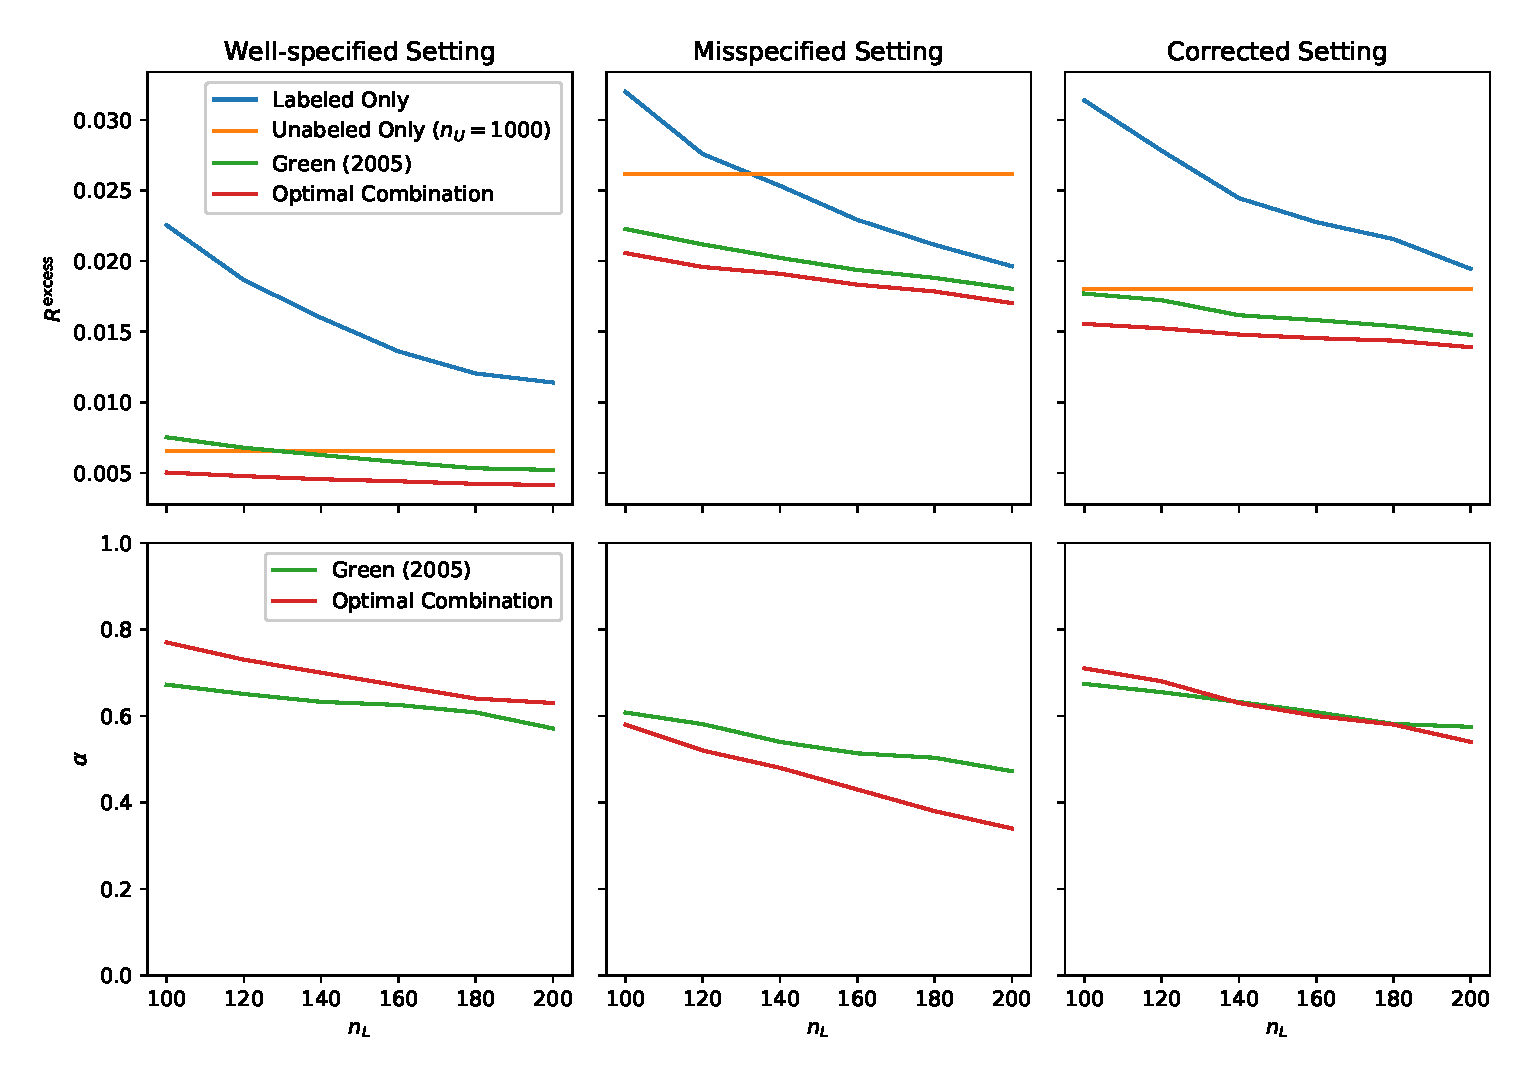
\includegraphics[width=.6\textwidth]{eps_figures/combined_with_alphas.eps}
    %
    \caption{Excess generalization error and associated combination weight $\alpha$ for an optimally weighted combination of labeled and unlabeled estimators, and a combination weighted according to \cite{GreenStrawderman2001} across the well-specified (left), misspecified (center), and corrected (right) settings. The number of unlabeled points is fixed at $n_U=1000$.}
    \label{fig:combined_with_alphas}
\end{figure}

\subsection{Real-World Case Study: Weak Supervision}

We discuss the weak supervision dataset we create and clarify the details of our experimental protocol for the real-world case study.

\paragraph{Creating a weak supervision dataset}

In weak supervision, soft labels from latent variable estimation are used as an alternative to a hand-labeled dataset. The sources used are usually heuristics which incorporate domain-specific knowledge about a particular task and can be acquired relatively cheaply. For our real-world case study, we choose the simple sentiment analysis task of classifying IMDB reviews as positive or negative. Our sources are defined simply: for a collection of positive sentiment words, output ``yes'' if the word appears in the review and ``no'' otherwise; for a collection of negative sentiment words, similarly output ``no'' if the word appears and ``yes'' otherwise. The specific words used and their sentiments are reported in \autoref{tab:imdb_words}. We select these words because they are empirically predictive, appear relatively frequently in reviews and are intuitively associated with positive/negative reviews.

\begin{table}[t]
\vskip 0.15in
\renewcommand{\arraystretch}{1.25} % Default value: 1
\begin{center}
\begin{small}
\begin{tabular}{l|cccccccccccccr}
\hline
Word & love & like & good & great & best & excellent & terrible & worst & bad & better & could & would \\
\hline
Sentiment & + & + & + & + & + & + & - & - & - & - & - & - \\
\hline
\end{tabular}
\end{small}
\end{center}
\vskip -0.1in
\caption{The words used as sources for the real-world weak supervision task of classifying IMDB reviews as positive or negative.}
\label{tab:imdb_words}
\end{table}

\paragraph{\autoref{fig:real_biases_data_value_ratio} and \autoref{tab:real_combo}: Experiments with real data} We measure excess generalization error, the data value ratio and the performances of combined estimators for the real-world dataset. Our protocols for these experiments mirror those we used for synthetic datasets, with two key differences: (1) for each trial, we sample points uniformly from the training set of 40,000 points, since we cannot sample directly from the distribution and (2) we measure generalization error on the test set, since we cannot compute the expected generalization error directly.


%\section{Maximum likelihood estimation without conditional abstain probabilities has a degenerate solution when every labeling function is unipolar}
\label{appendix:degenerate_solution}

We show that the maximum likelihood estimate for $\alpha$ under the probability model proposed by \cite{Ratner16} is degenerate when every labeling function is unipolar. This model considers the probability that labeling functions abstain equally across different classes, stating that the probability of observing labeling function outputs $z$ with gold label $y$ is
\begin{equation*}
    \text{Pr}_{\alpha,\beta}[\lambda_j(X)=z\mid Y=y]=\begin{cases}
        \alpha_j\beta_j&\text{ if }z=y\\
        (1-\alpha_j)\beta_j&\text{ if }z=-y\\
        (1-\beta_j)&\text{ if }z=0
    \end{cases}
\end{equation*}
Under this model we can write the log-likelihood as
\begin{align*}
    \ell_\text{unlabeled}(\boldsymbol{X}_U,\lambda,\alpha,\beta)&=\log\prod_{i=1}^{n_U}\text{Pr}_{\alpha,\beta}[\lambda(X)=\lambda(x^i_U)]\\
    &=\sum_{i=1}^{n_U}\log\sum_{y'\in\{-1,1\}}\text{Pr}_{\alpha,\beta}[\lambda(X)=\lambda(x^i_U), Y=y']\\
    &=\sum_{i=1}^{n_U}\log\sum_{y'\in\{-1,1\}}\text{Pr}[Y=y']\cdot\prod_{j=1}^m\text{Pr}_{\alpha,\beta}[\lambda_j(X)=\lambda_j(x^i_U)\mid Y=y']\\
    &=\sum_{i=1}^{n_U}\log\sum_{y'\in\{-1,1\}}\text{Pr}[Y=y']\cdot\prod_{j=1}^m\begin{cases}
        \alpha_j\beta_j&\text{ if }\lambda_j(x^i_U)=y'\\
        (1-\alpha_j)\beta_j&\text{ if }\lambda_j(x^i_U)=-y'\\
        (1-\beta_j)&\text{ if }\lambda_j(x^i_U)=0
    \end{cases}\\
    &=\sum_{i=1}^{n_U}\log\sum_{y'\in\{-1,1\}}\text{Pr}[Y=y']\cdot\prod_{j=1}^m\begin{cases}
        \beta_j&\text{ if }\lvert\lambda_j(x^i_U)\rvert=1\\
        1-\beta_j&\text{ if }\lambda_j(x^i_U)=0
    \end{cases}\\
    &\qquad\cdot\begin{cases}
        \alpha_j&\text{ if }\lambda_j(x^i_U)=y'\\
        1-\alpha_j&\text{ if }\lambda_j(x^i_U)=-y'\\
        1&\text{ if }\lambda_j(x^i_U)=0
    \end{cases}\\
    &=\sum_{i=1}^{n_U}\log\prod_{j=1}^m\begin{cases}
        \beta_j&\text{ if }\lvert\lambda_j(x^i_U)\rvert=1\\
        1-\beta_j&\text{ if }\lambda_j(x^i_U)=0
    \end{cases}\\
    &\qquad+\log\sum_{y'\in\{-1,1\}}\text{Pr}[Y=y']\cdot\prod_{j=1}^m\begin{cases}
        \alpha_j&\text{ if }\lambda_j(x^i_U)=y'\\
        1-\alpha_j&\text{ if }\lambda_j(x^i_U)=-y'\\
        1&\text{ if }\lambda_j(x^i_U)=0
    \end{cases}\\
    &=\ell_\text{coverages}(\boldsymbol{X}_U,\lambda,\beta)+\ell_\text{accuracies}(\boldsymbol{X}_U,\lambda,\alpha)
\end{align*}
where
\begin{equation*}
    \ell_\text{coverages}(\boldsymbol{X}_U,\lambda,\beta)=\sum_{i=1}^{n_U}\sum_{j=1}^m\log\begin{cases}
        \beta_j&\text{ if }\lvert\lambda_j(x^i_U)\rvert=1\\
        1-\beta_j&\text{ if }\lambda_j(x^i_U)=0
    \end{cases}
\end{equation*}
and
\begin{equation*}
    \ell_\text{accuracies}(\boldsymbol{X}_U,\lambda,\alpha)=\sum_{i=1}^{n_U}\log\sum_{y'\in\{-1,1\}}\text{Pr}[Y=y']\cdot\prod_{j=1}^m\begin{cases}
        \alpha_j&\text{ if }\lambda_j(x^i_U)=y'\\
        1-\alpha_j&\text{ if }\lambda_j(x^i_U)=-y'\\
        1&\text{ if }\lambda_j(x^i_U)=0
    \end{cases}
\end{equation*}
Hence the maximum likelihood estimates of $\alpha$ and $\beta$ are those which maximize $\ell_\text{accuracies}$ and $\ell_\text{coverages}$, respectively. The expression for $\ell_\text{coverages}$ is just the sum of the log-likelihood functions for $m$ Bernoulli random variables, meaning that the optimal value for each $\beta_j$ is the empirical coverage of $\lambda_j$ on the training set. Now, let $y_m$ be the majority class.
\begin{equation*}
    y_m=\argmax_y\text{Pr}[Y=y]
\end{equation*}
and let $\alpha^*$ be the estimate which assigns accuracy $1$ to every labeling function which outputs class $y_m$ and accuracy $0$ to every labeling function which outputs class $1-y_m$.
\begin{equation*}
    \alpha^*_j=\begin{cases}
        1&\text{ if }\text{class}(\lambda_j)=y_m\\
        0&\text{ otherwise}
    \end{cases}
\end{equation*}
We will show that $\alpha^*$ maximizes $\ell_\text{accuracies}$ and is thus the degenerate solution to this maximum likelihood estimation model. For each $x^i_U$, we consider two cases. If at least one labeling function fires, then let $j_\text{fires}$ denote the index of the labeling function which fires. Then
\begin{align*}
    &\sum_{y'\in\{-1,1\}}\text{Pr}[Y=y']\cdot\prod_{j=1}^m\begin{cases}
        \alpha_j&\text{ if }\lambda_j(x^i_U)=y'\\
        1-\alpha_j&\text{ if }\lambda_j(x^i_U)=-y'\\
        1&\text{ if }\lambda_j(x^i_U)=0
    \end{cases}\\
    \leq&\sum_{y'\in\{-1,1\}}\text{Pr}[Y=y']\cdot\begin{cases}
        \alpha_{j_\text{fires}}&\text{ if }\lambda_{j_\text{fires}}(x^i_U)=y'\\
        1-\alpha_{j_\text{fires}}&\text{ if }\lambda_{j_\text{fires}}(x^i_U)=-y'
    \end{cases}\\
    \leq&\text{Pr}[Y=y_m]\\
    =&\sum_{y'\in\{-1,1\}}\text{Pr}[Y=y']\cdot\begin{cases}
        1&\text{ if }y'=y_m\\
        0&\text{ otherwise}
    \end{cases}\\
    =&\sum_{y'\in\{-1,1\}}\text{Pr}[Y=y']\cdot\prod_{i=1}^m\begin{cases}
        \alpha^*_j&\text{ if }\lambda_j(x^i_U)=y'\\
        1-\alpha^*_j&\text{ if }\lambda_j(x^i_U)=-y'\\
        1&\text{ if }\lambda_j(x^i_U)=0
    \end{cases}
\end{align*}
If no labeling function fires, then
\begin{align*}
    &\sum_{y'\in\{-1,1\}}\text{Pr}[Y=y']\cdot\prod_{j=1}^m\begin{cases}
        \alpha_j&\text{ if }\lambda_j(x^i_U)=y'\\
        1-\alpha_j&\text{ if }\lambda_j(x^i_U)=-y'\\
        1&\text{ if }\lambda_j(x^i_U)=0
    \end{cases}\\
    =&\sum_{y'\in\{-1,1\}}\text{Pr}[Y=y']\\
    =&1\\
\end{align*}
In each case, the maximum value attained by this expression occurs at the degenerate solution $\alpha^*$, which completes our proof.

\section{Unipolar labeling function probability model}
\label{appendix:unipolar_probs}

We derive the following probability model for unipolar labeling functions.
\begin{align}
    \text{Pr}_{\alpha,\beta}[\lambda_j(X)=z\mid Y=c_j]&=\begin{cases}
        \alpha_j\beta_j/\text{Pr}[Y=c_j]&\text{ if }z=c_j\\
        1-\alpha_j\beta_j/\text{Pr}[Y=c_j]&\text{ if }z=0
    \end{cases}\\
    \text{Pr}_{\alpha,\beta}[\lambda_j(X)=z\mid Y=-c_j]&=\begin{cases}
        (1-\alpha_j)\beta_j/\text{Pr}[Y=-c_j]&\text{ if }z=c_j\\
        1-(1-\alpha_j)\beta_j/\text{Pr}[Y=-c_j]&\text{ if }z=0
    \end{cases}
\end{align}
First, we examine the case where $Y=c_j$. We know that $\lambda_j(X)=Y$ if and only if both $\lambda_j(X)=c_j$ and $Y=c_j$. This allows us to write
\begin{align*}
    \text{Pr}_{\alpha,\beta}[\lambda_j(X)=c_j\mid Y=c_j]&=\frac{\text{Pr}_{\alpha,\beta}[\lambda_j(X)=c_j, Y=c_j]}{\text{Pr}[Y=c_j]}\\
    &=\frac{\text{Pr}_{\alpha,\beta}[\lambda_j(X)=Y]}{\text{Pr}[Y=c_j]}\\
    &=\frac{\text{Pr}_{\alpha,\beta}[\lambda_j(X)=Y\mid\lvert \lambda_j(X)\rvert=1]\cdot\text{Pr}_{\alpha,\beta}[\lvert \lambda_j(X)\rvert=1]}{\text{Pr}[Y=c_j]}\\
    &=\alpha_j\beta_j/\text{Pr}[Y=c_j]
\end{align*}
We know that because $\lambda_j$ is unipolar
\begin{equation*}
    \text{Pr}_{\alpha,\beta}[\lambda_j(X)=-c_j\mid Y=c_j]=0
\end{equation*}
which means that
\begin{equation*}
    \text{Pr}_{\alpha,\beta}[\lambda_j(X)=0\mid Y=c_j]=1-\alpha_j\beta_j/\text{Pr}[Y=c_j]
\end{equation*}
Second, we examine the case where $Y=-c_j$. We know that $\lambda_j(X)=-Y$ if and only if both $z=c_j$ and $y=-c_j$. This means that
\begin{align*}
    \text{Pr}_{\alpha,\beta}[\lambda_j(X)=c_j\mid Y=-c_j]&=\frac{\text{Pr}_{\alpha,\beta}[\lambda_j(X)=c_j, Y=-c_j]}{\text{Pr}[Y=-c_j]}\\
    &=\frac{\text{Pr}_{\alpha,\beta}[\lambda_j(X)=-Y]}{\text{Pr}[Y=-c_j]}\\
    &=\frac{\text{Pr}_{\alpha,\beta}[\lambda_j(X)=-Y\mid\lvert \lambda_j(X)\rvert=1]\cdot\text{Pr}_{\alpha,\beta}[\lvert \lambda_j(X)\rvert=1]}{\text{Pr}[Y=-c_j]}\\
    &=\frac{(1-\text{Pr}_{\alpha,\beta}[\lambda_j(X)=Y\mid\lvert \lambda_j(X)\rvert=1])\cdot\text{Pr}_{\alpha,\beta}[\lvert \lambda_j(X)\rvert=1]}{\text{Pr}[Y=-c_j]}\\
    &=(1-\alpha_j)\beta_j/\text{Pr}[Y=-c_j]
\end{align*}
Similarly to before we know that
\begin{equation*}
    \text{Pr}_{\alpha,\beta}[\lambda_j(X)=-c_j\mid Y=-c_j]=0
\end{equation*}
and thus
\begin{equation*}
    \text{Pr}_{\alpha,\beta}[\lambda_j(X)=0\mid Y=-c_j]=1-(1-\alpha_j)\beta_j/\text{Pr}[Y=-c_j]
\end{equation*}

\section{Computing the Labeled Data Value Ratio}
\label{appendix:ldvr_computation}

To estimate the labeled data value ratio with parameters $\alpha_\text{mean},\beta_\text{mean}$ and $m$ we produce $100$ datasets. For each dataset, we randomly sample $n$ data points for $n\in\{100, 200, \hdots,10000\}$, train an unlabeled model and labeled model on these points, and evaluate the accuracy of each model over a test set of size $10000$. We compute the average accuracy for each value of $n$ over the $100$ datasets. Finally, we estimate the labeled data value according to
\begin{equation}
    \hat{r}=\argmin_r\sum_{n\in\{500,600,\hdots,10,000\}}\lvert \bar{A}_\text{unlabeled}(n)-\bar{A}_\text{labeled}(n/r)\rvert
\end{equation}
where $\bar{A}_\text{unlabeled}(n)$ is the mean performance of the unlabeled model trained on $n$ data points and $\bar{A}_\text{labeled}(n/r)$ is the mean performance of the labeled model trained on $n/r$ data points (interpolating linearly where $n/r\notin\{100,200,\hdots,10000\}$. We compute a single estimate $\hat{r}$ over the different values of $n$ because we find that the labeled data value generalizes across $n$, with $A_\text{unlabeled}(n)$ and $A_\text{labeled}(n/\hat{r})$ being close for different values of $n$. We choose to start at $n=500$ in the above expression because the accuracy gaps between consecutive values of $n$ for low $n$ are very large making these values of $n$ disproportionally important to our estimate of $r$.


\end{document}
